% Options for packages loaded elsewhere
\PassOptionsToPackage{unicode}{hyperref}
\PassOptionsToPackage{hyphens}{url}
\PassOptionsToPackage{dvipsnames,svgnames,x11names}{xcolor}
%
\documentclass[
  letterpaper,
  DIV=11,
  numbers=noendperiod]{scrreprt}

\usepackage{amsmath,amssymb}
\usepackage{iftex}
\ifPDFTeX
  \usepackage[T1]{fontenc}
  \usepackage[utf8]{inputenc}
  \usepackage{textcomp} % provide euro and other symbols
\else % if luatex or xetex
  \usepackage{unicode-math}
  \defaultfontfeatures{Scale=MatchLowercase}
  \defaultfontfeatures[\rmfamily]{Ligatures=TeX,Scale=1}
\fi
\usepackage{lmodern}
\ifPDFTeX\else  
    % xetex/luatex font selection
\fi
% Use upquote if available, for straight quotes in verbatim environments
\IfFileExists{upquote.sty}{\usepackage{upquote}}{}
\IfFileExists{microtype.sty}{% use microtype if available
  \usepackage[]{microtype}
  \UseMicrotypeSet[protrusion]{basicmath} % disable protrusion for tt fonts
}{}
\makeatletter
\@ifundefined{KOMAClassName}{% if non-KOMA class
  \IfFileExists{parskip.sty}{%
    \usepackage{parskip}
  }{% else
    \setlength{\parindent}{0pt}
    \setlength{\parskip}{6pt plus 2pt minus 1pt}}
}{% if KOMA class
  \KOMAoptions{parskip=half}}
\makeatother
\usepackage{xcolor}
\setlength{\emergencystretch}{3em} % prevent overfull lines
\setcounter{secnumdepth}{5}
% Make \paragraph and \subparagraph free-standing
\ifx\paragraph\undefined\else
  \let\oldparagraph\paragraph
  \renewcommand{\paragraph}[1]{\oldparagraph{#1}\mbox{}}
\fi
\ifx\subparagraph\undefined\else
  \let\oldsubparagraph\subparagraph
  \renewcommand{\subparagraph}[1]{\oldsubparagraph{#1}\mbox{}}
\fi

\usepackage{color}
\usepackage{fancyvrb}
\newcommand{\VerbBar}{|}
\newcommand{\VERB}{\Verb[commandchars=\\\{\}]}
\DefineVerbatimEnvironment{Highlighting}{Verbatim}{commandchars=\\\{\}}
% Add ',fontsize=\small' for more characters per line
\usepackage{framed}
\definecolor{shadecolor}{RGB}{241,243,245}
\newenvironment{Shaded}{\begin{snugshade}}{\end{snugshade}}
\newcommand{\AlertTok}[1]{\textcolor[rgb]{0.68,0.00,0.00}{#1}}
\newcommand{\AnnotationTok}[1]{\textcolor[rgb]{0.37,0.37,0.37}{#1}}
\newcommand{\AttributeTok}[1]{\textcolor[rgb]{0.40,0.45,0.13}{#1}}
\newcommand{\BaseNTok}[1]{\textcolor[rgb]{0.68,0.00,0.00}{#1}}
\newcommand{\BuiltInTok}[1]{\textcolor[rgb]{0.00,0.23,0.31}{#1}}
\newcommand{\CharTok}[1]{\textcolor[rgb]{0.13,0.47,0.30}{#1}}
\newcommand{\CommentTok}[1]{\textcolor[rgb]{0.37,0.37,0.37}{#1}}
\newcommand{\CommentVarTok}[1]{\textcolor[rgb]{0.37,0.37,0.37}{\textit{#1}}}
\newcommand{\ConstantTok}[1]{\textcolor[rgb]{0.56,0.35,0.01}{#1}}
\newcommand{\ControlFlowTok}[1]{\textcolor[rgb]{0.00,0.23,0.31}{#1}}
\newcommand{\DataTypeTok}[1]{\textcolor[rgb]{0.68,0.00,0.00}{#1}}
\newcommand{\DecValTok}[1]{\textcolor[rgb]{0.68,0.00,0.00}{#1}}
\newcommand{\DocumentationTok}[1]{\textcolor[rgb]{0.37,0.37,0.37}{\textit{#1}}}
\newcommand{\ErrorTok}[1]{\textcolor[rgb]{0.68,0.00,0.00}{#1}}
\newcommand{\ExtensionTok}[1]{\textcolor[rgb]{0.00,0.23,0.31}{#1}}
\newcommand{\FloatTok}[1]{\textcolor[rgb]{0.68,0.00,0.00}{#1}}
\newcommand{\FunctionTok}[1]{\textcolor[rgb]{0.28,0.35,0.67}{#1}}
\newcommand{\ImportTok}[1]{\textcolor[rgb]{0.00,0.46,0.62}{#1}}
\newcommand{\InformationTok}[1]{\textcolor[rgb]{0.37,0.37,0.37}{#1}}
\newcommand{\KeywordTok}[1]{\textcolor[rgb]{0.00,0.23,0.31}{#1}}
\newcommand{\NormalTok}[1]{\textcolor[rgb]{0.00,0.23,0.31}{#1}}
\newcommand{\OperatorTok}[1]{\textcolor[rgb]{0.37,0.37,0.37}{#1}}
\newcommand{\OtherTok}[1]{\textcolor[rgb]{0.00,0.23,0.31}{#1}}
\newcommand{\PreprocessorTok}[1]{\textcolor[rgb]{0.68,0.00,0.00}{#1}}
\newcommand{\RegionMarkerTok}[1]{\textcolor[rgb]{0.00,0.23,0.31}{#1}}
\newcommand{\SpecialCharTok}[1]{\textcolor[rgb]{0.37,0.37,0.37}{#1}}
\newcommand{\SpecialStringTok}[1]{\textcolor[rgb]{0.13,0.47,0.30}{#1}}
\newcommand{\StringTok}[1]{\textcolor[rgb]{0.13,0.47,0.30}{#1}}
\newcommand{\VariableTok}[1]{\textcolor[rgb]{0.07,0.07,0.07}{#1}}
\newcommand{\VerbatimStringTok}[1]{\textcolor[rgb]{0.13,0.47,0.30}{#1}}
\newcommand{\WarningTok}[1]{\textcolor[rgb]{0.37,0.37,0.37}{\textit{#1}}}

\providecommand{\tightlist}{%
  \setlength{\itemsep}{0pt}\setlength{\parskip}{0pt}}\usepackage{longtable,booktabs,array}
\usepackage{calc} % for calculating minipage widths
% Correct order of tables after \paragraph or \subparagraph
\usepackage{etoolbox}
\makeatletter
\patchcmd\longtable{\par}{\if@noskipsec\mbox{}\fi\par}{}{}
\makeatother
% Allow footnotes in longtable head/foot
\IfFileExists{footnotehyper.sty}{\usepackage{footnotehyper}}{\usepackage{footnote}}
\makesavenoteenv{longtable}
\usepackage{graphicx}
\makeatletter
\def\maxwidth{\ifdim\Gin@nat@width>\linewidth\linewidth\else\Gin@nat@width\fi}
\def\maxheight{\ifdim\Gin@nat@height>\textheight\textheight\else\Gin@nat@height\fi}
\makeatother
% Scale images if necessary, so that they will not overflow the page
% margins by default, and it is still possible to overwrite the defaults
% using explicit options in \includegraphics[width, height, ...]{}
\setkeys{Gin}{width=\maxwidth,height=\maxheight,keepaspectratio}
% Set default figure placement to htbp
\makeatletter
\def\fps@figure{htbp}
\makeatother
\newlength{\cslhangindent}
\setlength{\cslhangindent}{1.5em}
\newlength{\csllabelwidth}
\setlength{\csllabelwidth}{3em}
\newlength{\cslentryspacingunit} % times entry-spacing
\setlength{\cslentryspacingunit}{\parskip}
\newenvironment{CSLReferences}[2] % #1 hanging-ident, #2 entry spacing
 {% don't indent paragraphs
  \setlength{\parindent}{0pt}
  % turn on hanging indent if param 1 is 1
  \ifodd #1
  \let\oldpar\par
  \def\par{\hangindent=\cslhangindent\oldpar}
  \fi
  % set entry spacing
  \setlength{\parskip}{#2\cslentryspacingunit}
 }%
 {}
\usepackage{calc}
\newcommand{\CSLBlock}[1]{#1\hfill\break}
\newcommand{\CSLLeftMargin}[1]{\parbox[t]{\csllabelwidth}{#1}}
\newcommand{\CSLRightInline}[1]{\parbox[t]{\linewidth - \csllabelwidth}{#1}\break}
\newcommand{\CSLIndent}[1]{\hspace{\cslhangindent}#1}

\KOMAoption{captions}{tableheading}
\makeatletter
\makeatother
\makeatletter
\@ifpackageloaded{bookmark}{}{\usepackage{bookmark}}
\makeatother
\makeatletter
\@ifpackageloaded{caption}{}{\usepackage{caption}}
\AtBeginDocument{%
\ifdefined\contentsname
  \renewcommand*\contentsname{Table of contents}
\else
  \newcommand\contentsname{Table of contents}
\fi
\ifdefined\listfigurename
  \renewcommand*\listfigurename{List of Figures}
\else
  \newcommand\listfigurename{List of Figures}
\fi
\ifdefined\listtablename
  \renewcommand*\listtablename{List of Tables}
\else
  \newcommand\listtablename{List of Tables}
\fi
\ifdefined\figurename
  \renewcommand*\figurename{Figure}
\else
  \newcommand\figurename{Figure}
\fi
\ifdefined\tablename
  \renewcommand*\tablename{Table}
\else
  \newcommand\tablename{Table}
\fi
}
\@ifpackageloaded{float}{}{\usepackage{float}}
\floatstyle{ruled}
\@ifundefined{c@chapter}{\newfloat{codelisting}{h}{lop}}{\newfloat{codelisting}{h}{lop}[chapter]}
\floatname{codelisting}{Listing}
\newcommand*\listoflistings{\listof{codelisting}{List of Listings}}
\makeatother
\makeatletter
\@ifpackageloaded{caption}{}{\usepackage{caption}}
\@ifpackageloaded{subcaption}{}{\usepackage{subcaption}}
\makeatother
\makeatletter
\@ifpackageloaded{tcolorbox}{}{\usepackage[skins,breakable]{tcolorbox}}
\makeatother
\makeatletter
\@ifundefined{shadecolor}{\definecolor{shadecolor}{rgb}{.97, .97, .97}}
\makeatother
\makeatletter
\makeatother
\makeatletter
\makeatother
\ifLuaTeX
  \usepackage{selnolig}  % disable illegal ligatures
\fi
\IfFileExists{bookmark.sty}{\usepackage{bookmark}}{\usepackage{hyperref}}
\IfFileExists{xurl.sty}{\usepackage{xurl}}{} % add URL line breaks if available
\urlstyle{same} % disable monospaced font for URLs
\hypersetup{
  pdftitle={CM3},
  pdfauthor={Dr Chris Wheadon},
  colorlinks=true,
  linkcolor={blue},
  filecolor={Maroon},
  citecolor={Blue},
  urlcolor={Blue},
  pdfcreator={LaTeX via pandoc}}

\title{CM3}
\author{Dr Chris Wheadon}
\date{2023-02-23}

\begin{document}
\maketitle
\ifdefined\Shaded\renewenvironment{Shaded}{\begin{tcolorbox}[interior hidden, boxrule=0pt, borderline west={3pt}{0pt}{shadecolor}, breakable, sharp corners, frame hidden, enhanced]}{\end{tcolorbox}}\fi

\renewcommand*\contentsname{Table of contents}
{
\hypersetup{linkcolor=}
\setcounter{tocdepth}{2}
\tableofcontents
}
\bookmarksetup{startatroot}

\hypertarget{course-notes-for-cm3}{%
\chapter*{Course Notes for CM3}\label{course-notes-for-cm3}}
\addcontentsline{toc}{chapter}{Course Notes for CM3}

\markboth{Course Notes for CM3}{Course Notes for CM3}

\url{https://www.education.ox.ac.uk/study/msc-educational-assessment/}

\textbf{MODULE 3: PSYCHOMETRICS AND ASSESSMENT ANALYSIS} This paper
builds on concepts introduced in the first two core papers and
constitutes the foundation of technical measurement and data analysis in
educational assessment. It is specifically focussed on psychometric
methods for the evaluation of assessment data and integrates these
technical aspects with the historical and philosophical underpinnings of
psychometrics. Students will be introduced to various psychometric
frameworks, including Classical Test Theory, Item Response theory and
Rasch Measurement Theory, their approaches to assessment reliability and
validity, as well as relevant criticisms of the frameworks. Students
will also gain hands-on experience of different psychometric analyses
using the R statistical software.

\bookmarksetup{startatroot}

\hypertarget{modern-tools-for-rasch-analysis}{%
\chapter{Modern Tools for Rasch
Analysis}\label{modern-tools-for-rasch-analysis}}

\textbf{Tools} The following tools are recommended for the course. They
are all free and open source with the exception of Github Copilot which
offers a free trial.

\textbf{R}

\url{https://cran.r-project.org/} Follow the standard installation of R.
If you have used R before make sure you update to the latest version.

Once you have installed R, you will need to install the following
packages before going any further. Installing a package is done by
typing the following command in the R console:

\begin{verbatim}
    install.packages("languageserver")
    install.packages("rmarkdown")
    install.packages("tidyverse")
\end{verbatim}

\textbf{Visual Studio Code}

\url{https://code.visualstudio.com/} Download and install the latest
build. You will then need to install two extensions. This guide explains
what an extension is, and how to install it:
\url{https://code.visualstudio.com/docs/editor/extension-marketplace}

\textbf{VSCode extension: R}

\url{https://marketplace.visualstudio.com/items?itemName=REditorSupport.r}
The extension suggests various optional enhancements that you can
install, but these are not neccessary if you are using Quarto.

\textbf{VSCode extension: Quarto}

\url{https://marketplace.visualstudio.com/items?itemName=quarto.quarto}

\textbf{VSCode settings: Install httpgd in VSCode}

In VSCode: Code - Preferences - Settings - Extensions - R - Plot: Use
Httpgd.

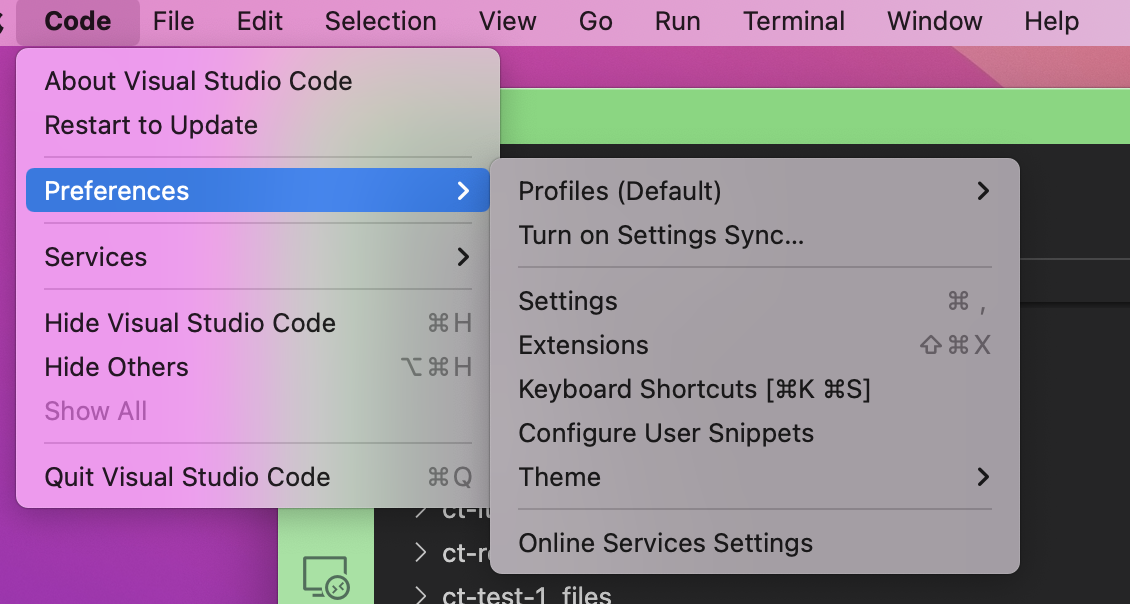
\includegraphics{images/plot-1.png} 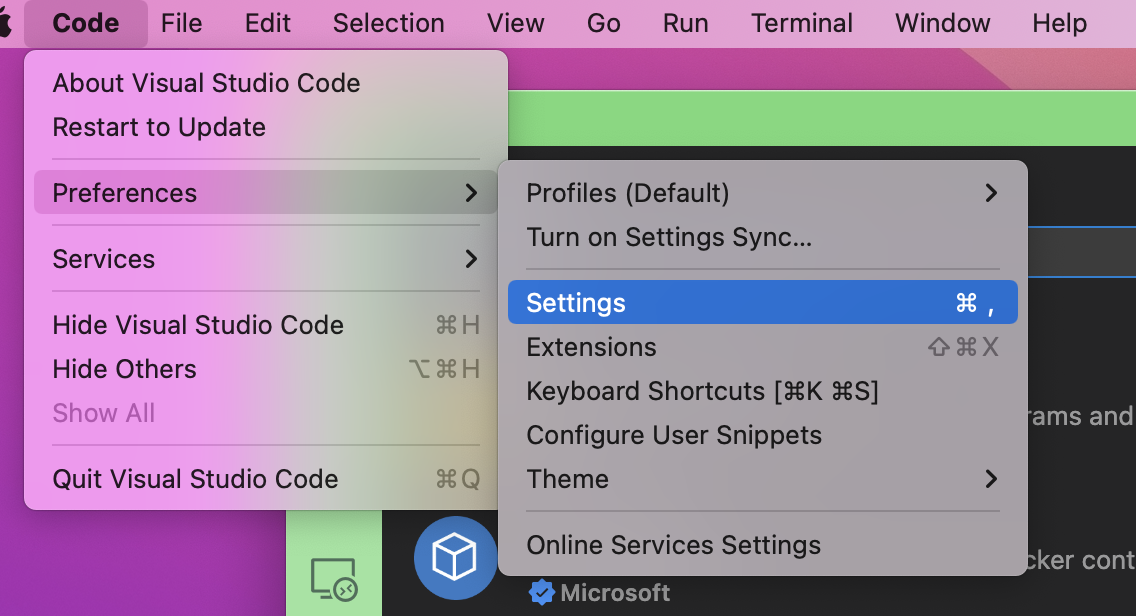
\includegraphics{images/plot-2.png}
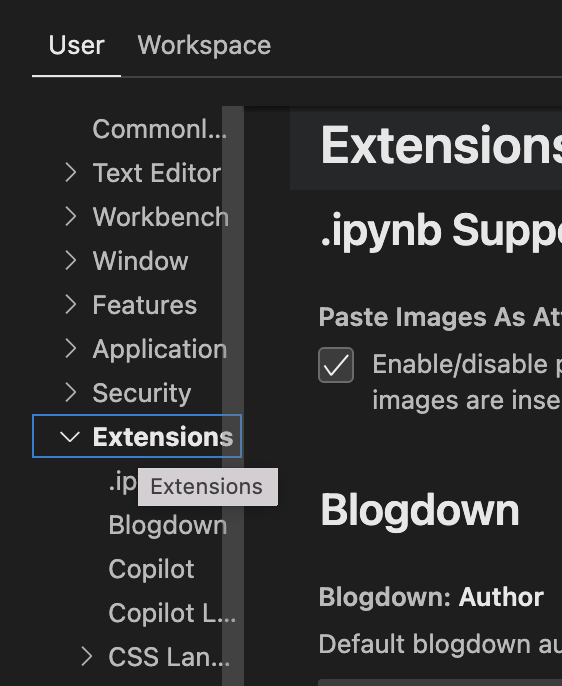
\includegraphics{images/plot-3.png} 
\includegraphics{images/plot-4.png}

In R:

\begin{verbatim}
    install.packages("httpgd")
\end{verbatim}

\textbf{Install Quarto}

https://quarto.org/docs/get-started/

You will need to close and reopen Visual Studio Code after installing
Quarto.

\textbf{OPTIONAL!}

\textbf{Github Copilot}

\url{https://copilot.github.com/} Copilot is an AI pair programmer. As
you type copilot will make suggestions for your code which will
accelerate your learning experience. Copilot offers a 60 day free trial.
To sign up for Copilot you will first need a free Github account.

\textbf{Github Copilot for Visual Studio Code}

\url{https://docs.github.com/en/copilot/getting-started-with-github-copilot/getting-started-with-github-copilot-in-visual-studio-code}
Once you have signed up for copilot you will need to install the
extension in Visual Studio Code.

\bookmarksetup{startatroot}

\hypertarget{verifying-your-installation}{%
\chapter{Verifying your
installation}\label{verifying-your-installation}}

Once you have installed your tools, you should be able to recreate the
example shown here: \url{https://quarto.org/docs/computations/r.html}

Inside VS Code, click on View - Command Palette and type ``Quarto: New
Document'' to create a new Quarto document.

\begin{figure}

{\centering 
\includegraphics{images/Screenshot 2023-02-23 at 11.11.03.png}

}

\caption{Command Palette}

\end{figure}

Then look for Render in the upper right hand corner. You will be
prompted to install any missing packages. If you need to do this you
need to open an R terminal in Visual Studio. Go to View - Command
Palette and type ``R: Create R Terminal''. This will open a new terminal
in the bottom of the screen. You can then type the following commands:

\begin{verbatim}
install.packages("rmarkdown")
install.packages("tidyverse")
\end{verbatim}

You should then be able to paste the code from the example into your new
document and run it. Along the way you will be prompted to install any
missing packages.

\textbf{Exercises}

\begin{enumerate}
\def\labelenumi{\arabic{enumi}.}
\item
  Using the example above, create one new Quarto document for each of
  the three built-in formats: HTML, PDF and Word. Render each of the
  three documents. How do the outputs differ? How do the inputs differ?
  (You may need to install LaTeX in order to build the PDF output ---
  Quarto will prompt you if this is necessary.)
\item
  Try out some markdown in your quarto document. Use
  \url{https://quarto.org/docs/authoring/markdown-basics.html} to get a
  feel for markdown. Try and do the following:
\end{enumerate}

\begin{itemize}
\tightlist
\item
  Embed an image
\item
  Create a table
\item
  Create a list
\item
  Create a link
\item
  Create an equation
\item
  Create an R code block and solve the equation 23 + 45
\end{itemize}

\begin{enumerate}
\def\labelenumi{\arabic{enumi}.}
\setcounter{enumi}{2}
\tightlist
\item
  Go to \url{https://r4ds.hadley.nz/} and work through until you reach
  2.2.5 Exercises.
\end{enumerate}

\bookmarksetup{startatroot}

\hypertarget{introduction-to-comparative-judgement}{%
\chapter{Introduction to Comparative
Judgement}\label{introduction-to-comparative-judgement}}

\hypertarget{what-is-comparative-judgement}{%
\subsection{What is Comparative
Judgement?}\label{what-is-comparative-judgement}}

\url{https://www.nomoremarking.com/demo?countryCode=GB}

\hypertarget{judging-writing}{%
\subsection{Judging writing}\label{judging-writing}}

\url{https://dev-cj.nomoremarking.com/judging/signup/989c5ad8-3682-4ad8-b8ba-c47fc49cc7c8}

Key points:

\begin{itemize}
\tightlist
\item
  reliability
\item
  scaled scores
\end{itemize}

\hypertarget{judging-numbers}{%
\subsection{Judging numbers}\label{judging-numbers}}

\url{https://dev-cj.nomoremarking.com/judging/signup/bd731049-e694-4644-b09b-a30dc9f8b440}

Key points:

\begin{itemize}
\tightlist
\item
  infit
\item
  probability
\end{itemize}

\part{Classical Test Theory}

\hypertarget{setting-up-your-analysis-environment}{%
\chapter{Setting up your analysis
environment}\label{setting-up-your-analysis-environment}}

\begin{itemize}
\tightlist
\item
  Create A New Folder called CM3
\item
  Start VS Code
\item
  Add the folder to workspace (CMD/CTRL + P + WORKSPACES ADD FOLDER TO
  WORKSPACE)
\item
  Create new quarto document (CMD/CTRL + P + QUARTO NEW DOCUMENT)
\item
  Download the data you need for the exercises:
  \url{https://cm3-datasets.s3.eu-west-1.amazonaws.com/data/data.zip}
\item
  Unzip the data to a new folder called data inside the CM3 folder
\end{itemize}

\hypertarget{the-dataset}{%
\chapter{The Dataset}\label{the-dataset}}

The dataset we will be using for analysis is a set of responses to a 20
question multiple choice test on sentence structure.

The test is designed to help teachers understand some of the most common
mistakes we see in their pupils' writing.

Here is a typical question.

\begin{center}\rule{0.5\linewidth}{0.5pt}\end{center}

\begin{quote}
\emph{Only one of the following sentences is correct. Select it.}
\end{quote}

\begin{quote}
\begin{enumerate}
\def\labelenumi{\Alph{enumi})}
\tightlist
\item
  Was very sorry about the mistake.
\end{enumerate}
\end{quote}

\begin{quote}
\begin{enumerate}
\def\labelenumi{\Alph{enumi})}
\setcounter{enumi}{1}
\tightlist
\item
  Gone away.
\end{enumerate}
\end{quote}

\begin{quote}
\begin{enumerate}
\def\labelenumi{\Alph{enumi})}
\setcounter{enumi}{2}
\tightlist
\item
  Skipped down the road.
\end{enumerate}
\end{quote}

\begin{quote}
\begin{enumerate}
\def\labelenumi{\Alph{enumi})}
\setcounter{enumi}{3}
\tightlist
\item
  We kicked the ball round the park.
\end{enumerate}
\end{quote}

\begin{quote}
\begin{enumerate}
\def\labelenumi{\Alph{enumi})}
\setcounter{enumi}{4}
\tightlist
\item
  Jumped over the fence.
\end{enumerate}
\end{quote}

\begin{center}\rule{0.5\linewidth}{0.5pt}\end{center}

You can download the full test here:
\url{https://cm3-datasets.s3.eu-west-1.amazonaws.com/data/Mid-year-test.docx}

\hypertarget{test-information}{%
\chapter{Test Information}\label{test-information}}

\begin{Shaded}
\begin{Highlighting}[]
\CommentTok{\# table with number of candidates, mean, standard deviation, min and max}
\CommentTok{\# round all stats to 2 decimal places}
\NormalTok{summary\_table }\OtherTok{\textless{}{-}}\NormalTok{ responses }\SpecialCharTok{\%\textgreater{}\%} 
  \FunctionTok{summarise}\NormalTok{(}
    \AttributeTok{n =} \FunctionTok{n}\NormalTok{(),}
    \AttributeTok{mean =} \FunctionTok{mean}\NormalTok{(total),}
    \AttributeTok{sd =} \FunctionTok{sd}\NormalTok{(total),}
    \AttributeTok{min =} \FunctionTok{min}\NormalTok{(total),}
    \AttributeTok{max =} \FunctionTok{max}\NormalTok{(total)}
\NormalTok{  )}
\NormalTok{knitr}\SpecialCharTok{::}\FunctionTok{kable}\NormalTok{(summary\_table, }\AttributeTok{digits =} \DecValTok{2}\NormalTok{,}\AttributeTok{align =} \StringTok{"c"}\NormalTok{)}
\end{Highlighting}
\end{Shaded}

\begin{longtable}[]{@{}ccccc@{}}
\toprule\noalign{}
n & mean & sd & min & max \\
\midrule\noalign{}
\endhead
\bottomrule\noalign{}
\endlastfoot
3061 & 12 & 4.03 & 0 & 20 \\
\end{longtable}

\hypertarget{score-distribution}{%
\chapter{Score Distribution}\label{score-distribution}}

\begin{Shaded}
\begin{Highlighting}[]
\FunctionTok{ggplot}\NormalTok{ (responses, }\FunctionTok{aes}\NormalTok{(}\AttributeTok{x =}\NormalTok{ total)) }\SpecialCharTok{+}
  \FunctionTok{geom\_histogram}\NormalTok{(}\AttributeTok{bins =} \DecValTok{21}\NormalTok{) }\SpecialCharTok{+}
  \FunctionTok{scale\_x\_continuous}\NormalTok{(}\AttributeTok{breaks =} \FunctionTok{seq}\NormalTok{(}\DecValTok{0}\NormalTok{, }\DecValTok{20}\NormalTok{, }\DecValTok{1}\NormalTok{)) }\SpecialCharTok{+}
  \CommentTok{\# add a vertical line at the mean}
    \FunctionTok{geom\_vline}\NormalTok{(}\AttributeTok{xintercept =} \FunctionTok{mean}\NormalTok{(responses}\SpecialCharTok{$}\NormalTok{total), }\AttributeTok{linetype =} \StringTok{"dashed"}\NormalTok{, }\AttributeTok{color =} \StringTok{"red"}\NormalTok{) }\SpecialCharTok{+}
    \CommentTok{\# add the light theme}
    \FunctionTok{theme\_light}\NormalTok{() }
\end{Highlighting}
\end{Shaded}

\begin{figure}[H]

{\centering 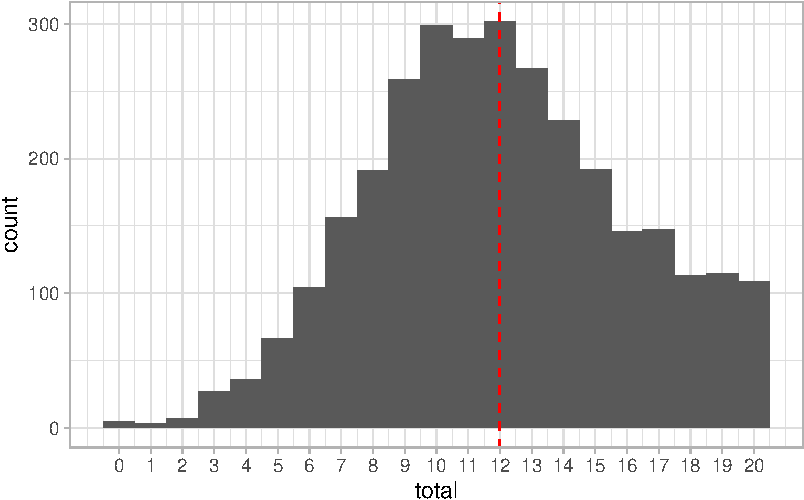
\includegraphics{ct-test-1_files/figure-pdf/fig-histogram-1.pdf}

}

\caption{\label{fig-histogram}Histogram of scores}

\end{figure}

\hypertarget{what-can-we-learn-from-the-distribution-of-scores}{%
\subsection{What can we learn from the distribution of
scores?}\label{what-can-we-learn-from-the-distribution-of-scores}}

\hypertarget{demographics}{%
\chapter{Demographics}\label{demographics}}

\hypertarget{working-with-demographic-data}{%
\subsection{Working with demographic
data}\label{working-with-demographic-data}}

In our dataset we have the the variable gender. Let's examine what sort
of variable gender is.

\begin{Shaded}
\begin{Highlighting}[]
\CommentTok{\# What class of variable is gender in the dataset?}
\FunctionTok{print}\NormalTok{(}\FunctionTok{class}\NormalTok{(responses}\SpecialCharTok{$}\NormalTok{gender))}
\end{Highlighting}
\end{Shaded}

\begin{verbatim}
[1] "character"
\end{verbatim}

To work with demographic data we need to convert the variable to a
factor. We can do this using the factor function.

\begin{Shaded}
\begin{Highlighting}[]
\CommentTok{\# List all the permutations of gender in the dataset}
\FunctionTok{print}\NormalTok{(}\FunctionTok{unique}\NormalTok{(responses}\SpecialCharTok{$}\NormalTok{gender))}
\end{Highlighting}
\end{Shaded}

\begin{verbatim}
[1] "F" "M" NA 
\end{verbatim}

\begin{Shaded}
\begin{Highlighting}[]
\NormalTok{responses }\OtherTok{\textless{}{-}}\NormalTok{ responses }\SpecialCharTok{\%\textgreater{}\%} 
  \FunctionTok{mutate\_at}\NormalTok{(}\FunctionTok{vars}\NormalTok{(gender), factor, }\AttributeTok{levels=}\FunctionTok{c}\NormalTok{(}\StringTok{\textquotesingle{}M\textquotesingle{}}\NormalTok{,}\StringTok{\textquotesingle{}F\textquotesingle{}}\NormalTok{),}\AttributeTok{labels=}\FunctionTok{c}\NormalTok{(}\StringTok{\textquotesingle{}Male\textquotesingle{}}\NormalTok{,}\StringTok{\textquotesingle{}Female\textquotesingle{}}\NormalTok{))}
\end{Highlighting}
\end{Shaded}

\hypertarget{what-are-the-proportions-of-male-female-in-the-dataset}{%
\section{What are the proportions of Male / Female in the
dataset?}\label{what-are-the-proportions-of-male-female-in-the-dataset}}

\begin{Shaded}
\begin{Highlighting}[]
\NormalTok{responses }\SpecialCharTok{\%\textgreater{}\%}
  \FunctionTok{group\_by}\NormalTok{(gender) }\SpecialCharTok{\%\textgreater{}\%}
  \FunctionTok{summarise}\NormalTok{(}\AttributeTok{n =} \FunctionTok{n}\NormalTok{()) }\SpecialCharTok{\%\textgreater{}\%}
  \FunctionTok{mutate}\NormalTok{(}\AttributeTok{freq =}\NormalTok{ n }\SpecialCharTok{/} \FunctionTok{sum}\NormalTok{(n))}
\end{Highlighting}
\end{Shaded}

\begin{verbatim}
# A tibble: 3 x 3
  gender     n    freq
  <fct>  <int>   <dbl>
1 Male    1527 0.499  
2 Female  1512 0.494  
3 <NA>      22 0.00719
\end{verbatim}

\hypertarget{remove-the-missing-data-for-simplicity}{%
\section{Remove the missing data for
simplicity}\label{remove-the-missing-data-for-simplicity}}

\begin{Shaded}
\begin{Highlighting}[]
\CommentTok{\# Remove the missing data for simplicity}
\NormalTok{responses }\OtherTok{\textless{}{-}}\NormalTok{ responses }\SpecialCharTok{\%\textgreater{}\%} \FunctionTok{drop\_na}\NormalTok{(gender)}
\end{Highlighting}
\end{Shaded}

\hypertarget{now-go-back-to-the-test-information-and-produce-a-table-and-a-histogram-by-gender}{%
\section{Now go back to the Test Information and produce a table and a
histogram by
gender}\label{now-go-back-to-the-test-information-and-produce-a-table-and-a-histogram-by-gender}}

\textbf{What do you learn from the grouped information?}

\hypertarget{descriptive-data}{%
\chapter{Descriptive Data}\label{descriptive-data}}

In the special case of dichotomous items, scored ``0'' for one response
and ``1'' for the other, the proportion of respondents in a sample who
select the response choice scored ``1'' is equivalent to the mean item
response. Items for which everyone gives the same response are
uninformative because they do not differentiate between individuals. In
contrast, dichotomous items that yield about an equal number of people
(50\%) selecting each of the two response options provide the best
differentiation between individuals in the sample overall (Cappelleri
(2014)).

\begin{Shaded}
\begin{Highlighting}[]
\CommentTok{\# select all the columns with \_score as the suffix and store as a tibble}
\NormalTok{items }\OtherTok{\textless{}{-}}\NormalTok{ responses }\SpecialCharTok{\%\textgreater{}\%} \FunctionTok{select}\NormalTok{(}\FunctionTok{ends\_with}\NormalTok{(}\StringTok{\textquotesingle{}\_score\textquotesingle{}}\NormalTok{))}

\CommentTok{\# pivot the items longer for analysis}
\NormalTok{items }\OtherTok{\textless{}{-}}\NormalTok{ items }\SpecialCharTok{\%\textgreater{}\%} \FunctionTok{pivot\_longer}\NormalTok{(}\AttributeTok{cols=}\FunctionTok{starts\_with}\NormalTok{(}\StringTok{\textquotesingle{}Q\textquotesingle{}}\NormalTok{), }\AttributeTok{names\_to =} \StringTok{\textquotesingle{}item\textquotesingle{}}\NormalTok{, }\AttributeTok{values\_to =} \StringTok{\textquotesingle{}score\textquotesingle{}}\NormalTok{)}

\CommentTok{\# create a summary table with item stats}
\NormalTok{item\_stats }\OtherTok{\textless{}{-}}\NormalTok{ items }\SpecialCharTok{\%\textgreater{}\%} 
  \FunctionTok{group\_by}\NormalTok{(item) }\SpecialCharTok{\%\textgreater{}\%}
  \FunctionTok{summarise}\NormalTok{(}\FunctionTok{across}\NormalTok{(}\FunctionTok{everything}\NormalTok{(), }
  \FunctionTok{list}\NormalTok{(}
    \AttributeTok{max =} \SpecialCharTok{\textasciitilde{}}\FunctionTok{max}\NormalTok{(.x, }\AttributeTok{na.rm =} \ConstantTok{TRUE}\NormalTok{),}
    \AttributeTok{n =} \SpecialCharTok{\textasciitilde{}}\FunctionTok{sum}\NormalTok{(}\SpecialCharTok{!}\FunctionTok{is.na}\NormalTok{(.x)),}
    \AttributeTok{mean =} \SpecialCharTok{\textasciitilde{}}\FunctionTok{mean}\NormalTok{(.x, }\AttributeTok{na.rm =} \ConstantTok{TRUE}\NormalTok{),}
    \AttributeTok{sd =} \SpecialCharTok{\textasciitilde{}}\FunctionTok{sd}\NormalTok{(.x, }\AttributeTok{na.rm =} \ConstantTok{TRUE}\NormalTok{)))}
\NormalTok{)}

\NormalTok{item\_stats }\OtherTok{\textless{}{-}}\NormalTok{ item\_stats }\SpecialCharTok{\%\textgreater{}\%} \FunctionTok{mutate}\NormalTok{(}
    \AttributeTok{item\_name =} \FunctionTok{factor}\NormalTok{(item, }\AttributeTok{levels=}\FunctionTok{paste}\NormalTok{(}\StringTok{\textquotesingle{}Q\textquotesingle{}}\NormalTok{,}\DecValTok{1}\SpecialCharTok{:}\DecValTok{20}\NormalTok{, }\StringTok{\textquotesingle{}\_score\textquotesingle{}}\NormalTok{,}\AttributeTok{sep=}\StringTok{\textquotesingle{}\textquotesingle{}}\NormalTok{),}\AttributeTok{labels =} \FunctionTok{paste0}\NormalTok{(}\StringTok{\textquotesingle{}Q\textquotesingle{}}\NormalTok{,}\DecValTok{1}\SpecialCharTok{:}\DecValTok{20}\NormalTok{),}\AttributeTok{ordered =} \ConstantTok{TRUE}\NormalTok{)}
\NormalTok{)}

\NormalTok{item\_stats }\OtherTok{\textless{}{-}}\NormalTok{ item\_stats }\SpecialCharTok{\%\textgreater{}\%} \FunctionTok{arrange}\NormalTok{(item\_name) }\SpecialCharTok{\%\textgreater{}\%}
    \FunctionTok{select}\NormalTok{(}
\NormalTok{        item\_name,}
\NormalTok{        score\_max,}
\NormalTok{        score\_n,}
\NormalTok{        score\_mean,}
\NormalTok{        score\_sd}
\NormalTok{    ) }\SpecialCharTok{\%\textgreater{}\%} \FunctionTok{rename}\NormalTok{(}
        \AttributeTok{Item =}\NormalTok{ item\_name,}
        \AttributeTok{Max =}\NormalTok{ score\_max,}
        \AttributeTok{N =}\NormalTok{ score\_n,}
        \AttributeTok{Mean =}\NormalTok{ score\_mean,}
        \AttributeTok{SD =}\NormalTok{ score\_sd}
\NormalTok{    )}

\CommentTok{\# display the summary table}
\NormalTok{knitr}\SpecialCharTok{::}\FunctionTok{kable}\NormalTok{(item\_stats, }\AttributeTok{digits=}\DecValTok{2}\NormalTok{)}
\end{Highlighting}
\end{Shaded}

\begin{longtable}[]{@{}lrrrr@{}}
\toprule\noalign{}
Item & Max & N & Mean & SD \\
\midrule\noalign{}
\endhead
\bottomrule\noalign{}
\endlastfoot
Q1 & 1 & 3049 & 0.95 & 0.22 \\
Q2 & 1 & 3039 & 0.93 & 0.25 \\
Q3 & 1 & 3049 & 0.66 & 0.47 \\
Q4 & 1 & 3050 & 0.94 & 0.24 \\
Q5 & 1 & 3050 & 0.90 & 0.30 \\
Q6 & 1 & 3047 & 0.39 & 0.49 \\
Q7 & 1 & 3037 & 0.31 & 0.46 \\
Q8 & 1 & 3039 & 0.33 & 0.47 \\
Q9 & 1 & 3046 & 0.59 & 0.49 \\
Q10 & 1 & 3046 & 0.79 & 0.41 \\
Q11 & 1 & 3043 & 0.82 & 0.38 \\
Q12 & 1 & 3040 & 0.59 & 0.49 \\
Q13 & 1 & 3036 & 0.67 & 0.47 \\
Q14 & 1 & 3045 & 0.72 & 0.45 \\
Q15 & 1 & 3042 & 0.18 & 0.38 \\
Q16 & 1 & 3039 & 0.30 & 0.46 \\
Q17 & 1 & 3039 & 0.55 & 0.50 \\
Q18 & 1 & 3022 & 0.63 & 0.48 \\
Q19 & 1 & 3036 & 0.26 & 0.44 \\
Q20 & 1 & 3034 & 0.55 & 0.50 \\
\end{longtable}

\hypertarget{item-discrimination}{%
\chapter{Item Discrimination}\label{item-discrimination}}

The more an item discriminates among individuals with different amounts
of the underlying concept of interest, the higher the discrimination
index.

\hypertarget{the-extreme-group-method-cappelleri}{%
\section{The extreme group method (Cappelleri
(2014))}\label{the-extreme-group-method-cappelleri}}

\hypertarget{step-1}{%
\subsection{Step 1}\label{step-1}}

Partition respondents who have the highest and lowest overall scores on
the overall scale, aggregated across all items, into upper and lower
groups. The upper group can be composed of the top x\% (e.g., 25\%) of
scores on the scale, while the lower group can be composed of the bottom
x\% (e.g., 25\%) of scores on the scale.

\begin{Shaded}
\begin{Highlighting}[]
\CommentTok{\# calculate the total score for each respondent}
\NormalTok{responses }\OtherTok{\textless{}{-}}\NormalTok{ responses }\SpecialCharTok{\%\textgreater{}\%} 
  \FunctionTok{mutate}\NormalTok{(}\AttributeTok{total =} \FunctionTok{rowSums}\NormalTok{(}\FunctionTok{pick}\NormalTok{(}\FunctionTok{ends\_with}\NormalTok{(}\StringTok{\textquotesingle{}\_score\textquotesingle{}}\NormalTok{)),}\AttributeTok{na.rm=}\ConstantTok{TRUE}\NormalTok{)) }

\CommentTok{\# partition the respondents into 4 quartiles based on their total score}
\NormalTok{responses }\OtherTok{\textless{}{-}}\NormalTok{ responses }\SpecialCharTok{\%\textgreater{}\%} 
  \FunctionTok{mutate}\NormalTok{(}\AttributeTok{quartile =} \FunctionTok{cut}\NormalTok{(total,}\FunctionTok{quantile}\NormalTok{(total,}\AttributeTok{probs=}\FunctionTok{c}\NormalTok{(}\DecValTok{0}\NormalTok{,}\FloatTok{0.25}\NormalTok{,}\FloatTok{0.5}\NormalTok{,}\FloatTok{0.75}\NormalTok{,}\DecValTok{1}\NormalTok{)),}\AttributeTok{labels=}\FunctionTok{c}\NormalTok{(}\StringTok{\textquotesingle{}Q1\textquotesingle{}}\NormalTok{,}\StringTok{\textquotesingle{}Q2\textquotesingle{}}\NormalTok{,}\StringTok{\textquotesingle{}Q3\textquotesingle{}}\NormalTok{,}\StringTok{\textquotesingle{}Q4\textquotesingle{}}\NormalTok{),}\AttributeTok{include.lowest=}\ConstantTok{TRUE}\NormalTok{))}

\CommentTok{\# double check}
\NormalTok{responses }\SpecialCharTok{\%\textgreater{}\%} 
  \FunctionTok{group\_by}\NormalTok{(quartile) }\SpecialCharTok{\%\textgreater{}\%} 
  \FunctionTok{summarise}\NormalTok{(}\AttributeTok{mean\_score =} \FunctionTok{mean}\NormalTok{(total))}
\end{Highlighting}
\end{Shaded}

\begin{verbatim}
# A tibble: 4 x 2
  quartile mean_score
  <fct>         <dbl>
1 Q1             7.20
2 Q2            11.0 
3 Q3            13.9 
4 Q4            17.8 
\end{verbatim}

\begin{Shaded}
\begin{Highlighting}[]
\NormalTok{items }\OtherTok{\textless{}{-}}\NormalTok{ responses }\SpecialCharTok{\%\textgreater{}\%} \FunctionTok{select}\NormalTok{(quartile, }\FunctionTok{ends\_with}\NormalTok{(}\StringTok{\textquotesingle{}\_score\textquotesingle{}}\NormalTok{))}
\CommentTok{\# pivot the items longer for analysis}
\NormalTok{items }\OtherTok{\textless{}{-}}\NormalTok{ items }\SpecialCharTok{\%\textgreater{}\%} \FunctionTok{pivot\_longer}\NormalTok{(}\SpecialCharTok{{-}}\NormalTok{quartile, }\AttributeTok{names\_to =} \StringTok{\textquotesingle{}item\textquotesingle{}}\NormalTok{, }\AttributeTok{values\_to =} \StringTok{\textquotesingle{}score\textquotesingle{}}\NormalTok{)}
\end{Highlighting}
\end{Shaded}

\hypertarget{step-2}{%
\subsection{Step 2}\label{step-2}}

Examine each item and determine the proportion of individual respondents
in the sample who correctly respond to each item in the upper group and
lower group.

\begin{Shaded}
\begin{Highlighting}[]
\CommentTok{\# create a summary table with item stats}
\NormalTok{item\_stats }\OtherTok{\textless{}{-}}\NormalTok{ items }\SpecialCharTok{\%\textgreater{}\%} 
  \FunctionTok{group\_by}\NormalTok{(quartile, item) }\SpecialCharTok{\%\textgreater{}\%}
  \FunctionTok{summarise}\NormalTok{(}\AttributeTok{mean\_score =} \FunctionTok{mean}\NormalTok{(score, }\AttributeTok{na.rm=}\ConstantTok{TRUE}\NormalTok{))}
\end{Highlighting}
\end{Shaded}

\begin{verbatim}
`summarise()` has grouped output by 'quartile'. You can override using the
`.groups` argument.
\end{verbatim}

\begin{Shaded}
\begin{Highlighting}[]
\CommentTok{\# pivot wider so we have the item stats for each quartile}
\NormalTok{item\_wide\_stats }\OtherTok{\textless{}{-}}\NormalTok{ item\_stats }\SpecialCharTok{\%\textgreater{}\%} 
  \FunctionTok{pivot\_wider}\NormalTok{(}\AttributeTok{names\_from =}\NormalTok{ quartile, }\AttributeTok{values\_from =}\NormalTok{ mean\_score)}

\NormalTok{item\_wide\_stats }\OtherTok{\textless{}{-}}\NormalTok{ item\_wide\_stats }\SpecialCharTok{\%\textgreater{}\%} \FunctionTok{mutate}\NormalTok{(}
    \AttributeTok{item\_name =} \FunctionTok{factor}\NormalTok{(item, }\AttributeTok{levels=}\FunctionTok{paste}\NormalTok{(}\StringTok{\textquotesingle{}Q\textquotesingle{}}\NormalTok{,}\DecValTok{1}\SpecialCharTok{:}\DecValTok{20}\NormalTok{, }\StringTok{\textquotesingle{}\_score\textquotesingle{}}\NormalTok{,}\AttributeTok{sep=}\StringTok{\textquotesingle{}\textquotesingle{}}\NormalTok{),}\AttributeTok{labels =} \FunctionTok{paste0}\NormalTok{(}\StringTok{\textquotesingle{}Q\textquotesingle{}}\NormalTok{,}\DecValTok{1}\SpecialCharTok{:}\DecValTok{20}\NormalTok{),}\AttributeTok{ordered =} \ConstantTok{TRUE}\NormalTok{)}
\NormalTok{    ) }\SpecialCharTok{\%\textgreater{}\%} \FunctionTok{arrange}\NormalTok{(item\_name) }

\NormalTok{item\_wide\_stats }\OtherTok{\textless{}{-}}\NormalTok{ item\_wide\_stats }\SpecialCharTok{\%\textgreater{}\%} \FunctionTok{select}\NormalTok{(}
\NormalTok{    item\_name, }
    \AttributeTok{Q1 =} \StringTok{\textasciigrave{}}\AttributeTok{Q1}\StringTok{\textasciigrave{}}\NormalTok{, }
    \AttributeTok{Q2 =} \StringTok{\textasciigrave{}}\AttributeTok{Q2}\StringTok{\textasciigrave{}}\NormalTok{, }
    \AttributeTok{Q3 =} \StringTok{\textasciigrave{}}\AttributeTok{Q3}\StringTok{\textasciigrave{}}\NormalTok{, }
    \AttributeTok{Q4 =} \StringTok{\textasciigrave{}}\AttributeTok{Q4}\StringTok{\textasciigrave{}}
\NormalTok{    )}
\end{Highlighting}
\end{Shaded}

\hypertarget{step-3}{%
\subsection{Step 3}\label{step-3}}

Subtract the pair of proportions noted in Step 2.

\begin{Shaded}
\begin{Highlighting}[]
\NormalTok{item\_wide\_stats }\OtherTok{\textless{}{-}}\NormalTok{ item\_wide\_stats }\SpecialCharTok{\%\textgreater{}\%} \FunctionTok{mutate}\NormalTok{(}
    \AttributeTok{Q1\_Q4 =}\NormalTok{ Q4 }\SpecialCharTok{{-}}\NormalTok{ Q1,}
\NormalTok{    )}
\NormalTok{knitr}\SpecialCharTok{::}\FunctionTok{kable}\NormalTok{(item\_wide\_stats, }\AttributeTok{digits=}\DecValTok{2}\NormalTok{)}
\end{Highlighting}
\end{Shaded}

\begin{longtable}[]{@{}lrrrrr@{}}
\toprule\noalign{}
item\_name & Q1 & Q2 & Q3 & Q4 & Q1\_Q4 \\
\midrule\noalign{}
\endhead
\bottomrule\noalign{}
\endlastfoot
Q1 & 0.85 & 0.98 & 0.99 & 1.00 & 0.14 \\
Q2 & 0.79 & 0.97 & 0.99 & 1.00 & 0.21 \\
Q3 & 0.33 & 0.65 & 0.82 & 0.95 & 0.62 \\
Q4 & 0.82 & 0.97 & 0.99 & 1.00 & 0.18 \\
Q5 & 0.74 & 0.93 & 0.96 & 1.00 & 0.26 \\
Q6 & 0.08 & 0.22 & 0.52 & 0.90 & 0.83 \\
Q7 & 0.08 & 0.15 & 0.35 & 0.81 & 0.73 \\
Q8 & 0.06 & 0.14 & 0.44 & 0.86 & 0.79 \\
Q9 & 0.21 & 0.48 & 0.85 & 0.98 & 0.77 \\
Q10 & 0.48 & 0.83 & 0.92 & 0.98 & 0.50 \\
Q11 & 0.57 & 0.84 & 0.95 & 0.98 & 0.41 \\
Q12 & 0.22 & 0.50 & 0.82 & 0.96 & 0.75 \\
Q13 & 0.41 & 0.66 & 0.78 & 0.92 & 0.51 \\
Q14 & 0.39 & 0.73 & 0.89 & 0.96 & 0.57 \\
Q15 & 0.05 & 0.07 & 0.13 & 0.54 & 0.49 \\
Q16 & 0.09 & 0.13 & 0.32 & 0.79 & 0.70 \\
Q17 & 0.31 & 0.52 & 0.62 & 0.85 & 0.53 \\
Q18 & 0.40 & 0.64 & 0.71 & 0.83 & 0.43 \\
Q19 & 0.06 & 0.09 & 0.26 & 0.77 & 0.71 \\
Q20 & 0.36 & 0.54 & 0.60 & 0.77 & 0.42 \\
\end{longtable}

\hypertarget{interpretation}{%
\section{Interpretation}\label{interpretation}}

The higher the item discrimination index, the more the item
discriminates. For example, if 60\% of the upper group and 25\% of the
lower group endorse a particular item in the scale, the item
discrimination index for that item would be calculated as (0.60−0.25) =
0.35.

\hypertarget{extension-exercise}{%
\section{Extension Exercise}\label{extension-exercise}}

Try and recreate the item discrimination plot
\href{https://www.ncbi.nlm.nih.gov/pmc/articles/PMC4096146/}{here}

\hypertarget{using-the-performance-package-for-item-discrimination}{%
\chapter{\texorpdfstring{Using the \emph{performance} package for item
discrimination}{Using the performance package for item discrimination}}\label{using-the-performance-package-for-item-discrimination}}

Rather than using our own home made functions, we can use the
\texttt{performance} package to calculate item discrimination. This is a
package that is designed for psychometrics, and has a number of useful
functions for calculating item statistics.

\begin{Shaded}
\begin{Highlighting}[]
\FunctionTok{library}\NormalTok{(performance)}
\FunctionTok{library}\NormalTok{(tidyverse)}
\end{Highlighting}
\end{Shaded}

\hypertarget{dichotomous-items}{%
\section{Dichotomous items}\label{dichotomous-items}}

\begin{Shaded}
\begin{Highlighting}[]
\CommentTok{\# load in the dataset}
\NormalTok{responses }\OtherTok{\textless{}{-}} \FunctionTok{read\_csv}\NormalTok{(}\StringTok{\textquotesingle{}data/responses.csv\textquotesingle{}}\NormalTok{)}
\CommentTok{\# select the columns we want}
\NormalTok{responses }\OtherTok{\textless{}{-}}\NormalTok{ responses }\SpecialCharTok{\%\textgreater{}\%} \FunctionTok{select}\NormalTok{(}\FunctionTok{contains}\NormalTok{(}\StringTok{\textquotesingle{}\_score\textquotesingle{}}\NormalTok{)) }
\end{Highlighting}
\end{Shaded}

\begin{Shaded}
\begin{Highlighting}[]
\CommentTok{\# item stats}
\NormalTok{item\_stats }\OtherTok{\textless{}{-}}\NormalTok{ performance}\SpecialCharTok{::}\FunctionTok{item\_reliability}\NormalTok{(responses)}
\NormalTok{knitr}\SpecialCharTok{::}\FunctionTok{kable}\NormalTok{(item\_stats)}
\end{Highlighting}
\end{Shaded}

\begin{longtable}[]{@{}lrr@{}}
\toprule\noalign{}
term & alpha\_if\_deleted & item\_discrimination \\
\midrule\noalign{}
\endhead
\bottomrule\noalign{}
\endlastfoot
Q1\_score & 0.808 & 0.252 \\
Q2\_score & 0.807 & 0.294 \\
Q3\_score & 0.801 & 0.398 \\
Q4\_score & 0.808 & 0.264 \\
Q5\_score & 0.807 & 0.284 \\
Q6\_score & 0.792 & 0.539 \\
Q7\_score & 0.796 & 0.476 \\
Q8\_score & 0.793 & 0.533 \\
Q9\_score & 0.794 & 0.515 \\
Q10\_score & 0.802 & 0.380 \\
Q11\_score & 0.804 & 0.338 \\
Q12\_score & 0.796 & 0.486 \\
Q13\_score & 0.807 & 0.305 \\
Q14\_score & 0.800 & 0.410 \\
Q15\_score & 0.802 & 0.391 \\
Q16\_score & 0.797 & 0.462 \\
Q17\_score & 0.807 & 0.302 \\
Q18\_score & 0.812 & 0.224 \\
Q19\_score & 0.796 & 0.496 \\
Q20\_score & 0.814 & 0.196 \\
\end{longtable}

\hypertarget{polytomous-items}{%
\section{Polytomous items}\label{polytomous-items}}

\begin{Shaded}
\begin{Highlighting}[]
\CommentTok{\# load in the dataset}
\NormalTok{responses }\OtherTok{\textless{}{-}} \FunctionTok{read\_csv}\NormalTok{(}\StringTok{\textquotesingle{}data/pc{-}data.csv\textquotesingle{}}\NormalTok{)}
\CommentTok{\# drop the first six columns}
\NormalTok{resp }\OtherTok{\textless{}{-}}\NormalTok{ responses }\SpecialCharTok{\%\textgreater{}\%} 
  \FunctionTok{select}\NormalTok{(}\SpecialCharTok{{-}}\FunctionTok{c}\NormalTok{(}\DecValTok{1}\SpecialCharTok{:}\DecValTok{6}\NormalTok{))}
\CommentTok{\# choose the columns that start with C1\_}
\NormalTok{resp\_c1 }\OtherTok{\textless{}{-}}\NormalTok{ resp }\SpecialCharTok{\%\textgreater{}\%} 
  \FunctionTok{select}\NormalTok{(}\FunctionTok{starts\_with}\NormalTok{(}\StringTok{\textquotesingle{}C1\_\textquotesingle{}}\NormalTok{))}
\end{Highlighting}
\end{Shaded}

\begin{Shaded}
\begin{Highlighting}[]
\CommentTok{\# load in the dataset}
\CommentTok{\# get the item stats}
\NormalTok{poly\_item\_stats }\OtherTok{\textless{}{-}}\NormalTok{ performance}\SpecialCharTok{::}\FunctionTok{item\_reliability}\NormalTok{(resp\_c1)}
\NormalTok{knitr}\SpecialCharTok{::}\FunctionTok{kable}\NormalTok{(poly\_item\_stats)}
\end{Highlighting}
\end{Shaded}

\begin{longtable}[]{@{}lrr@{}}
\toprule\noalign{}
term & alpha\_if\_deleted & item\_discrimination \\
\midrule\noalign{}
\endhead
\bottomrule\noalign{}
\endlastfoot
C1\_1ai & 0.850 & 0.147 \\
C1\_1aii & 0.848 & 0.296 \\
C1\_1bi & 0.851 & 0.105 \\
C1\_1bii & 0.848 & 0.276 \\
C1\_1biii & 0.846 & 0.355 \\
C1\_1biv & 0.847 & 0.396 \\
C1\_1ci & 0.846 & 0.370 \\
C1\_1cii & 0.842 & 0.479 \\
C1\_1di & 0.848 & 0.284 \\
C1\_1dii & 0.846 & 0.364 \\
C1\_1e & 0.839 & 0.543 \\
C1\_1eSPaG & 0.845 & 0.433 \\
C1\_2ai & 0.845 & 0.375 \\
C1\_2aii & 0.848 & 0.273 \\
C1\_2bi & 0.850 & 0.135 \\
C1\_2bii & 0.848 & 0.291 \\
C1\_2biii & 0.849 & 0.254 \\
C1\_2biv & 0.843 & 0.455 \\
C1\_2bv & 0.843 & 0.463 \\
C1\_2c & 0.837 & 0.606 \\
C1\_2d & 0.841 & 0.506 \\
C1\_3ai & 0.840 & 0.536 \\
C1\_3aii & 0.848 & 0.291 \\
C1\_3aiii & 0.844 & 0.408 \\
C1\_3bi & 0.850 & 0.117 \\
C1\_3bii & 0.843 & 0.437 \\
C1\_3ci & 0.845 & 0.384 \\
C1\_3cii & 0.838 & 0.563 \\
C1\_3d & 0.841 & 0.503 \\
\end{longtable}

\hypertarget{correlations}{%
\chapter{Correlations}\label{correlations}}

\hypertarget{item-total-correlations}{%
\section{Item Total Correlations}\label{item-total-correlations}}

Item total correlations, are generally used as supporting evidence for
the reliability of test forms. Items may be excluded from a test form if
they have a poor correlation to the total score. The item total
correlation is the correlation between the item score and the total
score.

\begin{Shaded}
\begin{Highlighting}[]
\CommentTok{\# correlate each item score with the total score}
\CommentTok{\# note that this function includes the studied item score in the total score for simplicity, but normally the item score would be excluded from the total score, see https://personality{-}project.org/r/html/alpha.html}
\NormalTok{item\_total\_r }\OtherTok{\textless{}{-}}\NormalTok{ responses }\SpecialCharTok{\%\textgreater{}\%} 
  \FunctionTok{select}\NormalTok{(}\FunctionTok{ends\_with}\NormalTok{(}\StringTok{"\_score"}\NormalTok{)) }\SpecialCharTok{\%\textgreater{}\%} 
  \FunctionTok{mutate}\NormalTok{(}\AttributeTok{total =}\NormalTok{ responses}\SpecialCharTok{$}\NormalTok{total) }\SpecialCharTok{\%\textgreater{}\%} 
  \FunctionTok{gather}\NormalTok{(}\AttributeTok{key =} \StringTok{"item"}\NormalTok{, }\AttributeTok{value =} \StringTok{"score"}\NormalTok{, }\SpecialCharTok{{-}}\NormalTok{total) }\SpecialCharTok{\%\textgreater{}\%} 
  \FunctionTok{mutate}\NormalTok{(}\AttributeTok{item =} \FunctionTok{str\_remove}\NormalTok{(item, }\StringTok{"\_score"}\NormalTok{)) }\SpecialCharTok{\%\textgreater{}\%} 
  \FunctionTok{group\_by}\NormalTok{(item) }\SpecialCharTok{\%\textgreater{}\%} 
  \FunctionTok{summarise}\NormalTok{(}\AttributeTok{correlation =} \FunctionTok{cor}\NormalTok{(score, total, }\AttributeTok{use =} \StringTok{"pairwise.complete.obs"}\NormalTok{)) }\SpecialCharTok{\%\textgreater{}\%} 
  \FunctionTok{arrange}\NormalTok{(}\FunctionTok{desc}\NormalTok{(correlation))}
  
\NormalTok{knitr}\SpecialCharTok{::}\FunctionTok{kable}\NormalTok{(item\_total\_r, }\AttributeTok{digits =} \DecValTok{2}\NormalTok{)}
\end{Highlighting}
\end{Shaded}

\hypertarget{tbl-itemr}{}
\begin{longtable}[]{@{}lr@{}}
\caption{\label{tbl-itemr}Item Total Correlations}\tabularnewline
\toprule\noalign{}
item & correlation \\
\midrule\noalign{}
\endfirsthead
\toprule\noalign{}
item & correlation \\
\midrule\noalign{}
\endhead
\bottomrule\noalign{}
\endlastfoot
Q6 & 0.62 \\
Q8 & 0.60 \\
Q9 & 0.60 \\
Q12 & 0.58 \\
Q19 & 0.56 \\
Q7 & 0.56 \\
Q16 & 0.54 \\
Q3 & 0.50 \\
Q14 & 0.50 \\
Q10 & 0.48 \\
Q15 & 0.45 \\
Q11 & 0.43 \\
Q13 & 0.41 \\
Q17 & 0.41 \\
Q2 & 0.37 \\
Q5 & 0.37 \\
Q18 & 0.34 \\
Q4 & 0.34 \\
Q20 & 0.32 \\
Q1 & 0.32 \\
\end{longtable}

\hypertarget{discussion}{%
\section{Discussion}\label{discussion}}

Is there a relationship between item difficulty and item total
correlation? Can you see any issues with excluding items based on item
total correlation?

\hypertarget{inter-item-correlations}{%
\section{Inter-item Correlations}\label{inter-item-correlations}}

\begin{Shaded}
\begin{Highlighting}[]
\NormalTok{x2 }\OtherTok{\textless{}{-}}\NormalTok{ responses }\SpecialCharTok{\%\textgreater{}\%} 
  \FunctionTok{select}\NormalTok{(}\FunctionTok{ends\_with}\NormalTok{(}\StringTok{"\_score"}\NormalTok{)) }\SpecialCharTok{\%\textgreater{}\%}
  \FunctionTok{correlate}\NormalTok{()}
\end{Highlighting}
\end{Shaded}

\begin{verbatim}
Correlation computed with
* Method: 'pearson'
* Missing treated using: 'pairwise.complete.obs'
\end{verbatim}

\begin{Shaded}
\begin{Highlighting}[]
\NormalTok{x2 }\SpecialCharTok{\%\textgreater{}\%} \FunctionTok{network\_plot}\NormalTok{(}\AttributeTok{min\_cor =}\NormalTok{ .}\DecValTok{1}\NormalTok{)}
\end{Highlighting}
\end{Shaded}

\begin{figure}[H]

{\centering 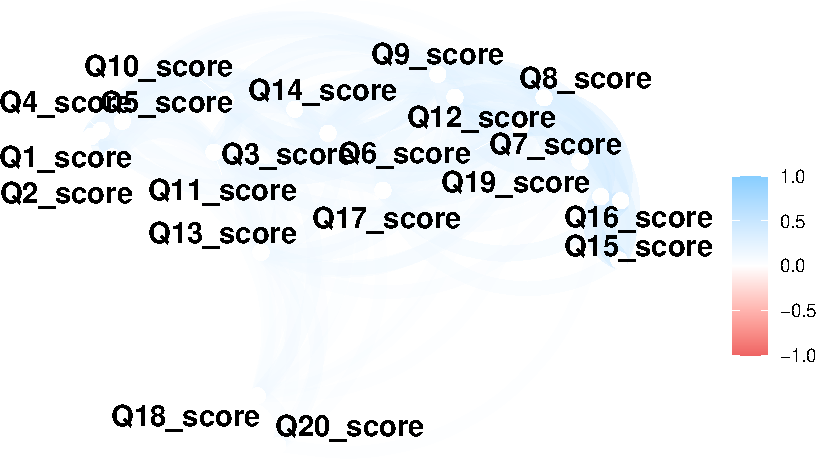
\includegraphics{ct-item-total-1_files/figure-pdf/network-plot-1.pdf}

}

\caption{Network diagram of inter-item correlations}

\end{figure}

\hypertarget{distractor-analysis-with-dexter}{%
\chapter{Distractor analysis with
dexter}\label{distractor-analysis-with-dexter}}

\begin{Shaded}
\begin{Highlighting}[]
\FunctionTok{rm}\NormalTok{(}\AttributeTok{list=}\FunctionTok{ls}\NormalTok{())}
\FunctionTok{library}\NormalTok{(tidyverse)}
\FunctionTok{library}\NormalTok{(dexter)}
\CommentTok{\# load in the dataset}
\NormalTok{responses }\OtherTok{\textless{}{-}} \FunctionTok{read\_csv}\NormalTok{(}\StringTok{\textquotesingle{}data/responses.csv\textquotesingle{}}\NormalTok{)}
\NormalTok{keys }\OtherTok{\textless{}{-}} \FunctionTok{read\_csv}\NormalTok{(}\StringTok{\textquotesingle{}data/key.csv\textquotesingle{}}\NormalTok{)}
\CommentTok{\# Create the rules}
\NormalTok{rules }\OtherTok{\textless{}{-}} \FunctionTok{keys\_to\_rules}\NormalTok{(keys, }\AttributeTok{include\_NA\_rule =} \ConstantTok{TRUE}\NormalTok{)}
\NormalTok{db }\OtherTok{\textless{}{-}} \FunctionTok{start\_new\_project}\NormalTok{(rules, }\AttributeTok{db\_name =} \StringTok{":memory:"}\NormalTok{, }\AttributeTok{person\_properties=}\FunctionTok{list}\NormalTok{(}\AttributeTok{gender=}\StringTok{"unknown"}\NormalTok{))}
\FunctionTok{add\_booklet}\NormalTok{(db, responses, }\StringTok{"y7"}\NormalTok{) }
\end{Highlighting}
\end{Shaded}

\begin{Shaded}
\begin{Highlighting}[]
\FunctionTok{get\_booklets}\NormalTok{(db)}
\end{Highlighting}
\end{Shaded}

\begin{verbatim}
  booklet_id n_items n_persons booklet_max_score
1         y7      20      3061                20
\end{verbatim}

\begin{Shaded}
\begin{Highlighting}[]
\FunctionTok{head}\NormalTok{(}\FunctionTok{get\_items}\NormalTok{(db))}
\end{Highlighting}
\end{Shaded}

\begin{verbatim}
  item_id
1      Q1
2     Q10
3     Q11
4     Q12
5     Q13
6     Q14
\end{verbatim}

\begin{Shaded}
\begin{Highlighting}[]
\FunctionTok{get\_persons}\NormalTok{(db) }\SpecialCharTok{\%\textgreater{}\%} 
  \FunctionTok{glimpse}\NormalTok{()}
\end{Highlighting}
\end{Shaded}

\begin{verbatim}
Rows: 3,061
Columns: 2
$ person_id <chr> "dx_0000001", "dx_0000002", "dx_0000003", "dx_0000004", "dx_~
$ gender    <chr> "F", "M", "F", "M", "M", "F", "M", "M", "F", "M", "F", "F", ~
\end{verbatim}

\begin{Shaded}
\begin{Highlighting}[]
\NormalTok{tt }\OtherTok{=} \FunctionTok{tia\_tables}\NormalTok{(db)}
\NormalTok{tt}\SpecialCharTok{$}\NormalTok{booklets}
\end{Highlighting}
\end{Shaded}

\begin{verbatim}
  booklet_id n_items     alpha mean_pvalue  mean_rit  mean_rir
1         y7      20 0.8137408    0.599755 0.4681555 0.3826158
  max_booklet_score n_persons
1                20      3061
\end{verbatim}

\begin{Shaded}
\begin{Highlighting}[]
\NormalTok{knitr}\SpecialCharTok{::}\FunctionTok{kable}\NormalTok{(tt}\SpecialCharTok{$}\NormalTok{items)}
\end{Highlighting}
\end{Shaded}

\begin{longtable}[]{@{}
  >{\raggedright\arraybackslash}p{(\columnwidth - 16\tabcolsep) * \real{0.1222}}
  >{\raggedright\arraybackslash}p{(\columnwidth - 16\tabcolsep) * \real{0.0889}}
  >{\raggedleft\arraybackslash}p{(\columnwidth - 16\tabcolsep) * \real{0.1222}}
  >{\raggedleft\arraybackslash}p{(\columnwidth - 16\tabcolsep) * \real{0.1111}}
  >{\raggedleft\arraybackslash}p{(\columnwidth - 16\tabcolsep) * \real{0.1111}}
  >{\raggedleft\arraybackslash}p{(\columnwidth - 16\tabcolsep) * \real{0.1111}}
  >{\raggedleft\arraybackslash}p{(\columnwidth - 16\tabcolsep) * \real{0.1111}}
  >{\raggedleft\arraybackslash}p{(\columnwidth - 16\tabcolsep) * \real{0.1111}}
  >{\raggedleft\arraybackslash}p{(\columnwidth - 16\tabcolsep) * \real{0.1111}}@{}}
\toprule\noalign{}
\begin{minipage}[b]{\linewidth}\raggedright
booklet\_id
\end{minipage} & \begin{minipage}[b]{\linewidth}\raggedright
item\_id
\end{minipage} & \begin{minipage}[b]{\linewidth}\raggedleft
mean\_score
\end{minipage} & \begin{minipage}[b]{\linewidth}\raggedleft
sd\_score
\end{minipage} & \begin{minipage}[b]{\linewidth}\raggedleft
max\_score
\end{minipage} & \begin{minipage}[b]{\linewidth}\raggedleft
pvalue
\end{minipage} & \begin{minipage}[b]{\linewidth}\raggedleft
rit
\end{minipage} & \begin{minipage}[b]{\linewidth}\raggedleft
rir
\end{minipage} & \begin{minipage}[b]{\linewidth}\raggedleft
n\_persons
\end{minipage} \\
\midrule\noalign{}
\endhead
\bottomrule\noalign{}
\endlastfoot
y7 & Q1 & 0.9460960 & 0.2258281 & 1 & 0.9460960 & 0.3334998 & 0.2822894
& 3061 \\
y7 & Q10 & 0.7817707 & 0.4130439 & 1 & 0.7817707 & 0.4890928 & 0.4051286
& 3061 \\
y7 & Q11 & 0.8160732 & 0.3874245 & 1 & 0.8160732 & 0.4369315 & 0.3542171
& 3061 \\
y7 & Q12 & 0.5870631 & 0.4923617 & 1 & 0.5870631 & 0.5774198 & 0.4869096
& 3061 \\
y7 & Q13 & 0.6644887 & 0.4721689 & 1 & 0.6644887 & 0.4167201 & 0.3128742
& 3061 \\
y7 & Q14 & 0.7170859 & 0.4504150 & 1 & 0.7170859 & 0.5027417 & 0.4120081
& 3061 \\
y7 & Q15 & 0.1754329 & 0.3803369 & 1 & 0.1754329 & 0.4521971 & 0.3722567
& 3061 \\
y7 & Q16 & 0.2969618 & 0.4569196 & 1 & 0.2969618 & 0.5363749 & 0.4479760
& 3061 \\
y7 & Q17 & 0.5508004 & 0.4974126 & 1 & 0.5508004 & 0.4103008 & 0.2999650
& 3061 \\
y7 & Q18 & 0.6229990 & 0.4846352 & 1 & 0.6229990 & 0.3456235 & 0.2334171
& 3061 \\
y7 & Q19 & 0.2606991 & 0.4390160 & 1 & 0.2606991 & 0.5611054 & 0.4793179
& 3061 \\
y7 & Q2 & 0.9235544 & 0.2657098 & 1 & 0.9235544 & 0.3706761 & 0.3117073
& 3061 \\
y7 & Q20 & 0.5485136 & 0.4976409 & 1 & 0.5485136 & 0.3256473 & 0.2089781
& 3061 \\
y7 & Q3 & 0.6602418 & 0.4736270 & 1 & 0.6602418 & 0.5033116 & 0.4075765
& 3061 \\
y7 & Q4 & 0.9340085 & 0.2482672 & 1 & 0.9340085 & 0.3441510 & 0.2881099
& 3061 \\
y7 & Q5 & 0.8961124 & 0.3051147 & 1 & 0.8961124 & 0.3780087 & 0.3103319
& 3061 \\
y7 & Q6 & 0.3868017 & 0.4870176 & 1 & 0.3868017 & 0.6149106 & 0.5308310
& 3061 \\
y7 & Q7 & 0.3074159 & 0.4614232 & 1 & 0.3074159 & 0.5552584 & 0.4681820
& 3061 \\
y7 & Q8 & 0.3299575 & 0.4701974 & 1 & 0.3299575 & 0.6029375 & 0.5203720
& 3061 \\
y7 & Q9 & 0.5890232 & 0.4920110 & 1 & 0.5890232 & 0.6062016 & 0.5198674
& 3061 \\
\end{longtable}

\hypertarget{distractor-plots}{%
\section{Distractor plots}\label{distractor-plots}}

\begin{Shaded}
\begin{Highlighting}[]
\CommentTok{\# Look at distractor plots for all items}
\NormalTok{n\_items }\OtherTok{\textless{}{-}} \FunctionTok{nrow}\NormalTok{(keys)}
\ControlFlowTok{for}\NormalTok{(i }\ControlFlowTok{in} \DecValTok{1}\SpecialCharTok{:}\NormalTok{n\_items)\{}
  \FunctionTok{distractor\_plot}\NormalTok{(db, keys}\SpecialCharTok{$}\NormalTok{item\_id[i])}
\NormalTok{\}}
\end{Highlighting}
\end{Shaded}

\begin{figure}[H]

{\centering \includegraphics{ct-distractors_files/figure-pdf/unnamed-chunk-3-1.pdf}

}

\end{figure}

\begin{figure}[H]

{\centering 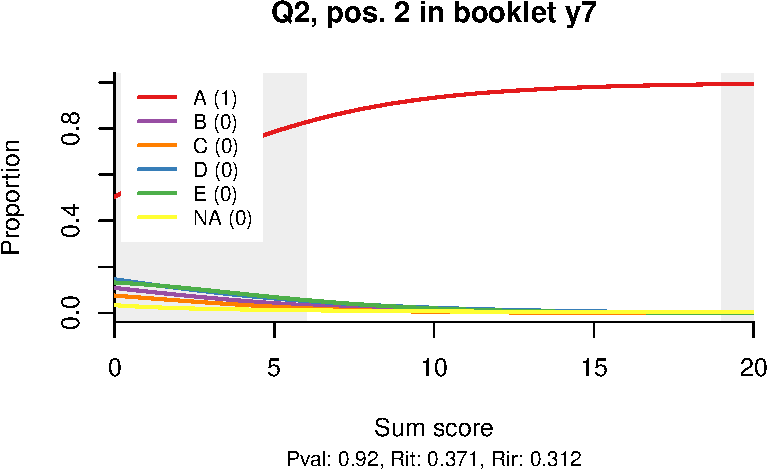
\includegraphics{ct-distractors_files/figure-pdf/unnamed-chunk-3-2.pdf}

}

\end{figure}

\begin{figure}[H]

{\centering 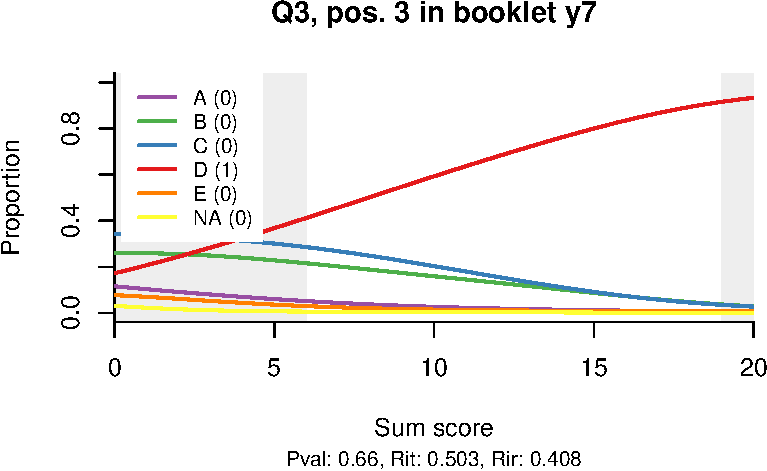
\includegraphics{ct-distractors_files/figure-pdf/unnamed-chunk-3-3.pdf}

}

\end{figure}

\begin{figure}[H]

{\centering 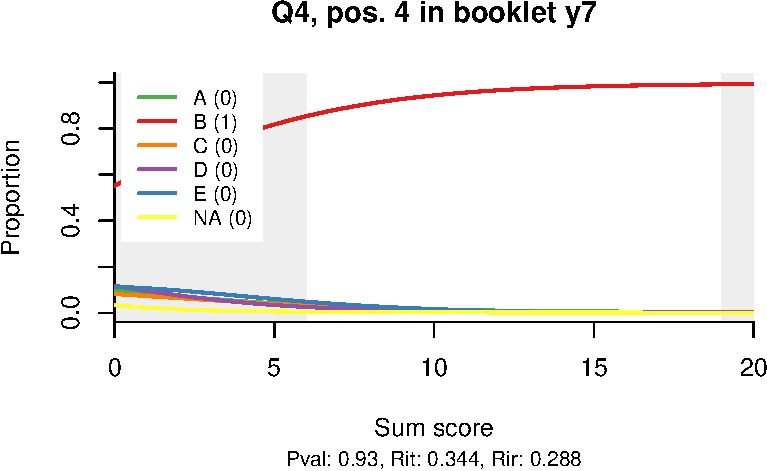
\includegraphics{ct-distractors_files/figure-pdf/unnamed-chunk-3-4.pdf}

}

\end{figure}

\begin{figure}[H]

{\centering 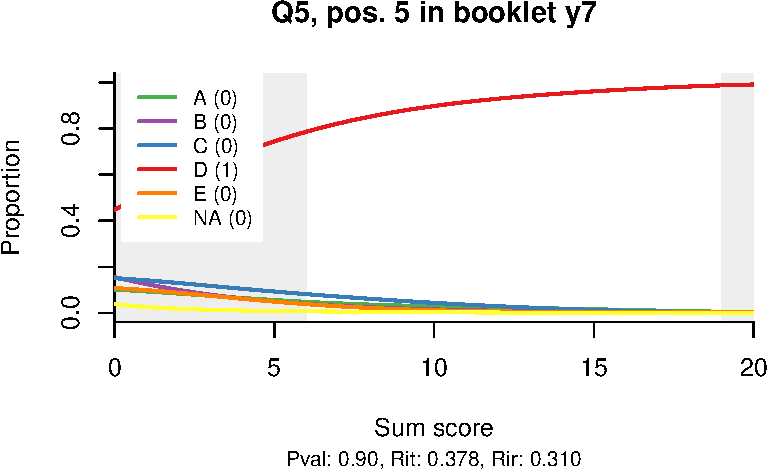
\includegraphics{ct-distractors_files/figure-pdf/unnamed-chunk-3-5.pdf}

}

\end{figure}

\begin{figure}[H]

{\centering 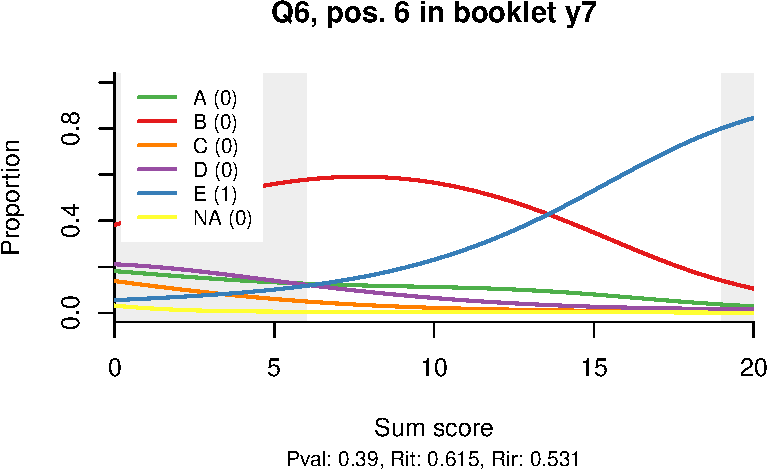
\includegraphics{ct-distractors_files/figure-pdf/unnamed-chunk-3-6.pdf}

}

\end{figure}

\begin{figure}[H]

{\centering 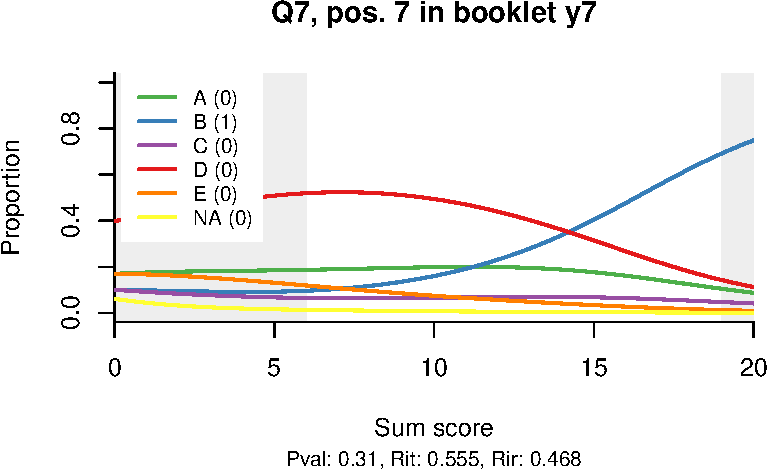
\includegraphics{ct-distractors_files/figure-pdf/unnamed-chunk-3-7.pdf}

}

\end{figure}

\begin{figure}[H]

{\centering 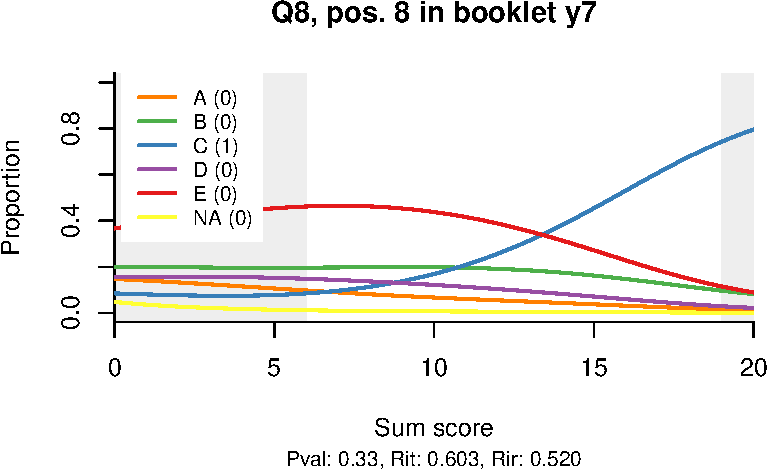
\includegraphics{ct-distractors_files/figure-pdf/unnamed-chunk-3-8.pdf}

}

\end{figure}

\begin{figure}[H]

{\centering 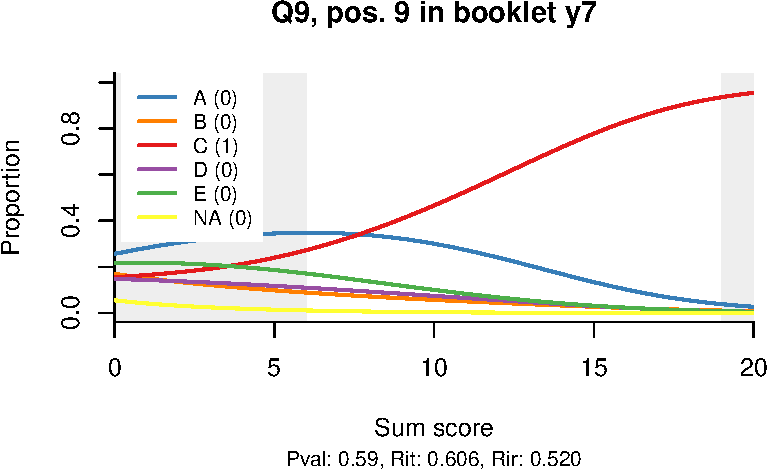
\includegraphics{ct-distractors_files/figure-pdf/unnamed-chunk-3-9.pdf}

}

\end{figure}

\begin{figure}[H]

{\centering 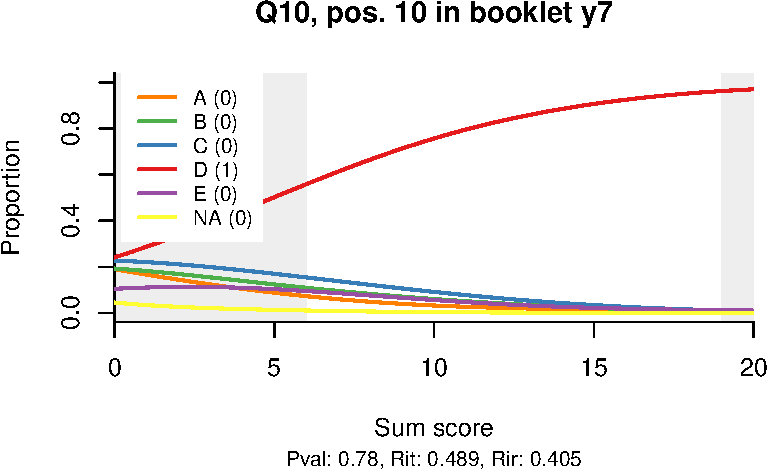
\includegraphics{ct-distractors_files/figure-pdf/unnamed-chunk-3-10.pdf}

}

\end{figure}

\begin{figure}[H]

{\centering 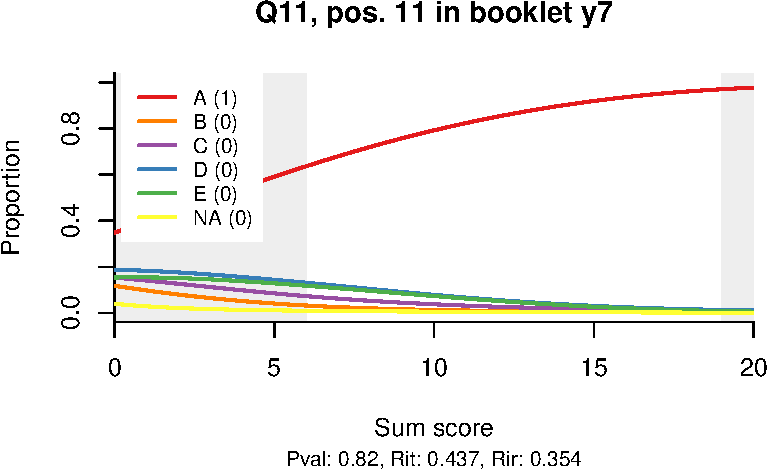
\includegraphics{ct-distractors_files/figure-pdf/unnamed-chunk-3-11.pdf}

}

\end{figure}

\begin{figure}[H]

{\centering 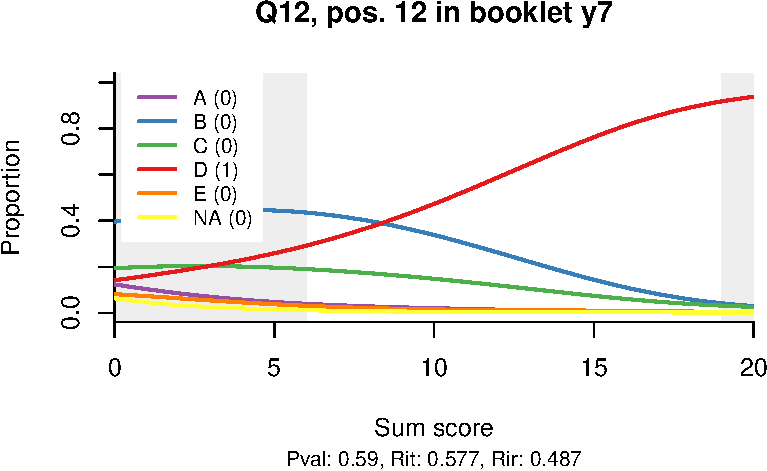
\includegraphics{ct-distractors_files/figure-pdf/unnamed-chunk-3-12.pdf}

}

\end{figure}

\begin{figure}[H]

{\centering 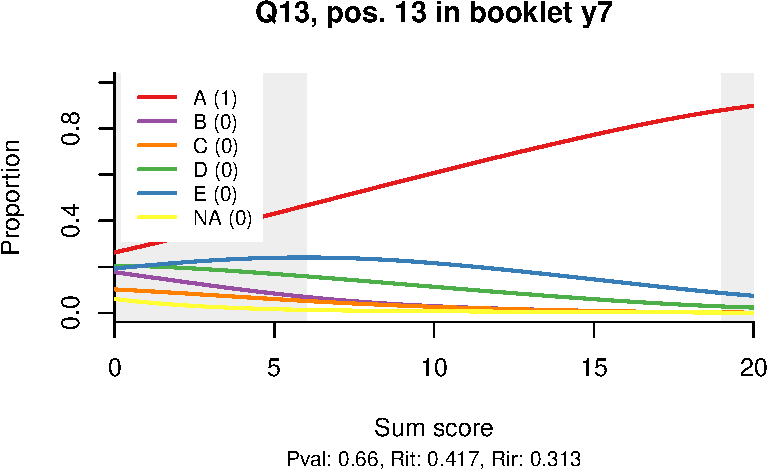
\includegraphics{ct-distractors_files/figure-pdf/unnamed-chunk-3-13.pdf}

}

\end{figure}

\begin{figure}[H]

{\centering 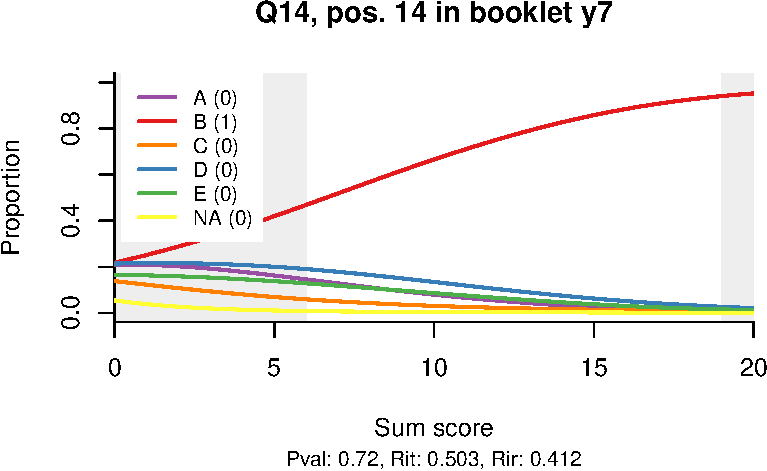
\includegraphics{ct-distractors_files/figure-pdf/unnamed-chunk-3-14.pdf}

}

\end{figure}

\begin{figure}[H]

{\centering 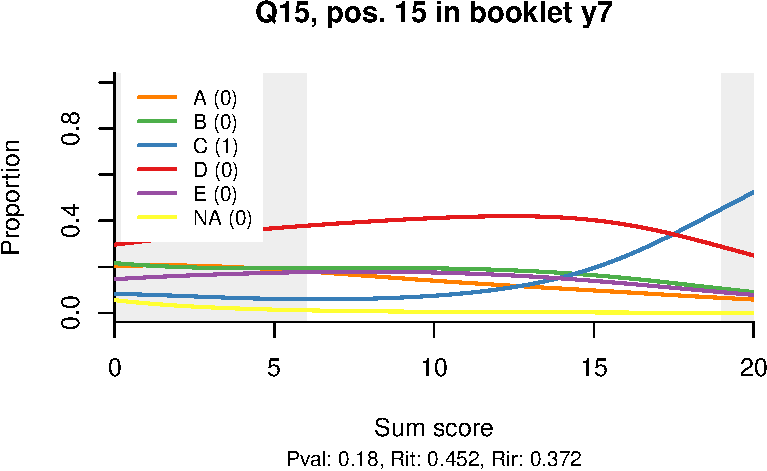
\includegraphics{ct-distractors_files/figure-pdf/unnamed-chunk-3-15.pdf}

}

\end{figure}

\begin{figure}[H]

{\centering 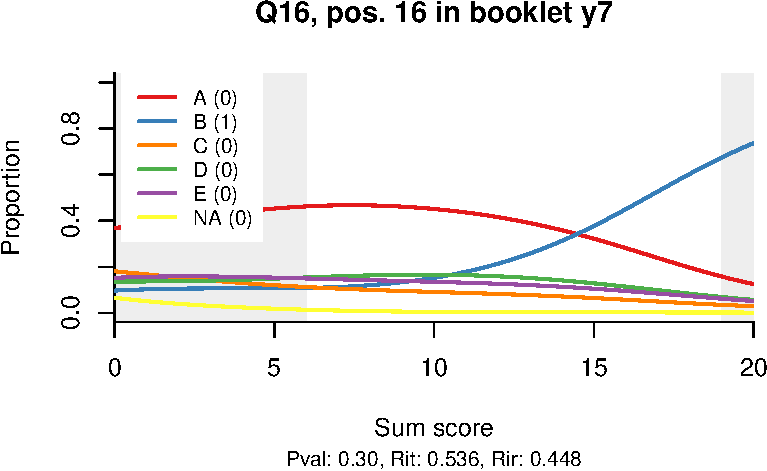
\includegraphics{ct-distractors_files/figure-pdf/unnamed-chunk-3-16.pdf}

}

\end{figure}

\begin{figure}[H]

{\centering 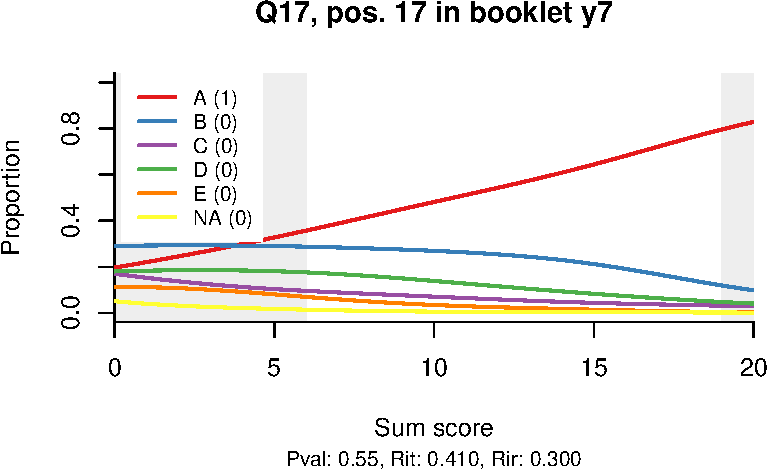
\includegraphics{ct-distractors_files/figure-pdf/unnamed-chunk-3-17.pdf}

}

\end{figure}

\begin{figure}[H]

{\centering 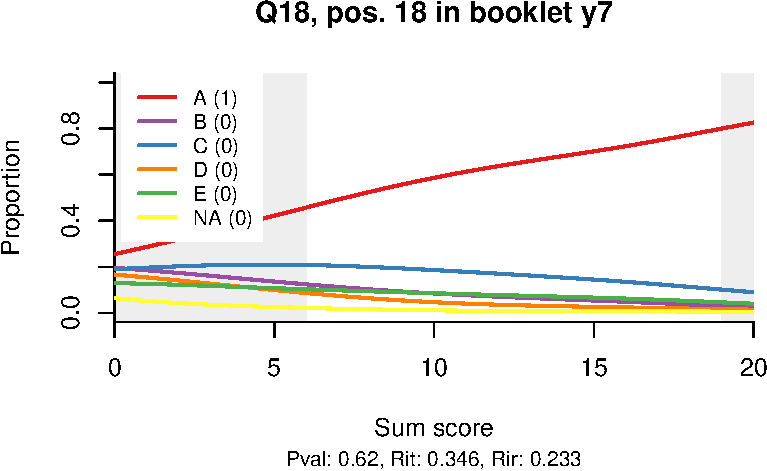
\includegraphics{ct-distractors_files/figure-pdf/unnamed-chunk-3-18.pdf}

}

\end{figure}

\begin{figure}[H]

{\centering 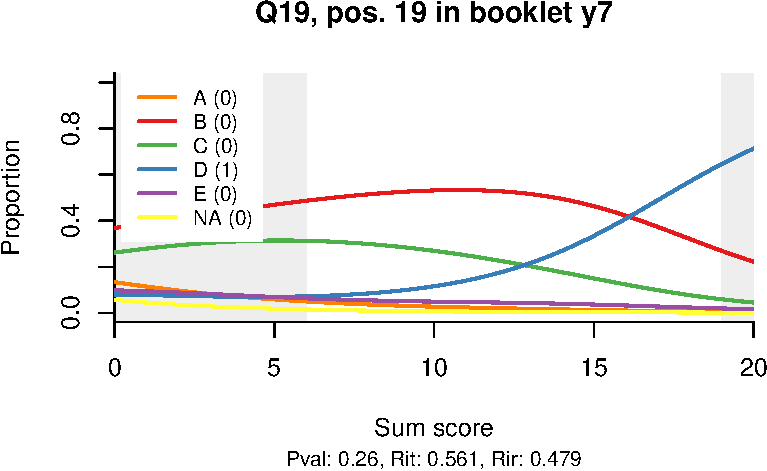
\includegraphics{ct-distractors_files/figure-pdf/unnamed-chunk-3-19.pdf}

}

\end{figure}

\begin{figure}[H]

{\centering 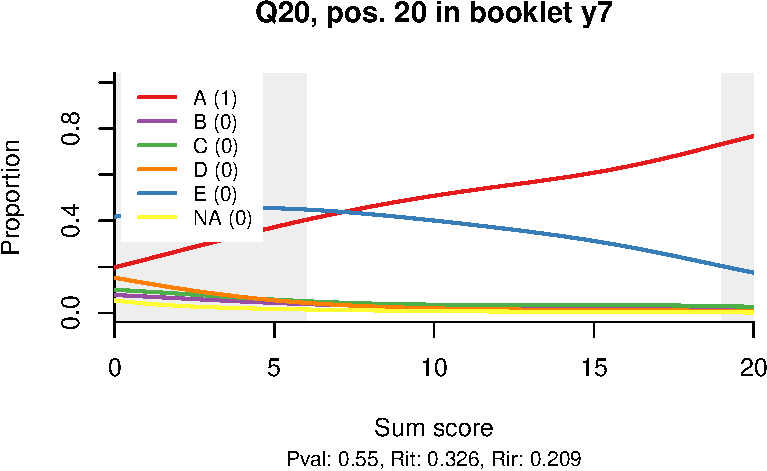
\includegraphics{ct-distractors_files/figure-pdf/unnamed-chunk-3-20.pdf}

}

\end{figure}

\hypertarget{analysis-questions}{%
\section{Analysis questions}\label{analysis-questions}}

Does the slope of the correct answer always rise from left to right?
Does the curve for the correct answer always rise above those for the
incorrect answers? What does the steepness of the slope for the correct
answer tell you about an item? Change the key so that one of the items
is incorrectly marked. What do you see in the distractor analysis? What
is the role of the curtains (the shaded areas in the plots)? Are there
any items where they are particularly helpful? How many distractors
generally seem to be useful? What would you typically expect the
probability of guessing the correct answer to be for a MC item with 5
choices? If you look at the point at which the distractors cross the
y-axis where sum score = 0, what do you learn about the actual
probabilities? Can you make any recommendations for improvement based on
the distractor analysis?

\begin{Shaded}
\begin{Highlighting}[]
\FunctionTok{close\_project}\NormalTok{(db)}
\end{Highlighting}
\end{Shaded}

\hypertarget{reliability}{%
\chapter{Reliability}\label{reliability}}

\hypertarget{observed-scores-true-scores-and-error}{%
\section{Observed Scores, True Scores and
Error}\label{observed-scores-true-scores-and-error}}

Classical Test Theory assumes that tests suffer from random measurement
error.

The test contains \emph{J} items. Random variable
\emph{X\textsubscript{j}} denotes the score on item \emph{j}. The
summary of the item scores is the total score or test score, which is
defined as

\[
X_+ = \sum_{j=1}^J X_j
\]

Test score \emph{X\textsubscript{+i}} is assumed to suffer from random
measurement error. Thus, rather than \emph{X\textsubscript{+i}} one
would like to know respondent \emph{i}'s test score without error. This
error-free test score is defined as the expectation of
\emph{X\textsubscript{+i}} across the propensity distribution of
independent repetitions of the test to individual \emph{i}, that is, as
ɛ(\emph{X\textsubscript{+i}}) (Lord \& Novick, 1968, pp.~29--30). The
expectation is better known as the true score.
\url{https://www.ncbi.nlm.nih.gov/pmc/articles/PMC2792363/}

The difference between a test score resulting from a single test
administration and the true score is defined to be the random
measurement error.

Reliability coefficients are an attempt to quantify the random
measurement error in the absence of infinite repetitions of tests.

The most widely used coefficient is
\href{https://link.springer.com/article/10.1007/bf02310555}{alpha}.
Mathematically, alpha depends on the average degree of inter-relatedness
between the items in a test and is heavily dependent on the number of
items in a test.

\hypertarget{exploring-alpha}{%
\chapter{Exploring alpha}\label{exploring-alpha}}

\begin{Shaded}
\begin{Highlighting}[]
\NormalTok{mdl\_alpha }\OtherTok{\textless{}{-}}\NormalTok{ psych}\SpecialCharTok{::}\FunctionTok{alpha}\NormalTok{(item\_responses)}
\FunctionTok{print}\NormalTok{(}\FunctionTok{summary}\NormalTok{(mdl\_alpha))}
\end{Highlighting}
\end{Shaded}

\begin{verbatim}

Reliability analysis   
 raw_alpha std.alpha G6(smc) average_r S/N    ase mean  sd median_r
      0.81      0.81    0.83      0.18 4.3 0.0048  0.6 0.2     0.16
NULL
\end{verbatim}

\textbf{What happens to alpha if you only use half the scores?}

\hypertarget{from-alpha-to-omega}{%
\section{From alpha to omega}\label{from-alpha-to-omega}}

\url{https://tidsskriftet.no/en/2022/08/medicine-and-numbers/internal-consistency-alpha-omega}

\begin{Shaded}
\begin{Highlighting}[]
\NormalTok{mdl\_omega }\OtherTok{\textless{}{-}}\NormalTok{ psych}\SpecialCharTok{::}\FunctionTok{omega}\NormalTok{(item\_responses)}
\end{Highlighting}
\end{Shaded}

\begin{verbatim}
Loading required namespace: GPArotation
\end{verbatim}

\begin{verbatim}
Warning in fa.stats(r = r, f = f, phi = phi, n.obs = n.obs, np.obs = np.obs, :
The estimated weights for the factor scores are probably incorrect.  Try a
different factor score estimation method.
\end{verbatim}

\begin{verbatim}
Warning in fac(r = r, nfactors = nfactors, n.obs = n.obs, rotate = rotate, : An
ultra-Heywood case was detected.  Examine the results carefully
\end{verbatim}

\begin{verbatim}
Warning in cov2cor(t(w) %*% r %*% w): diag(.) had 0 or NA entries; non-finite
result is doubtful
\end{verbatim}

\begin{figure}[H]

{\centering \includegraphics{ct-alpha_files/figure-pdf/unnamed-chunk-3-1.pdf}

}

\end{figure}

\begin{Shaded}
\begin{Highlighting}[]
\FunctionTok{print}\NormalTok{(}\FunctionTok{summary}\NormalTok{(mdl\_omega))}
\end{Highlighting}
\end{Shaded}

\begin{verbatim}
Omega 
psych::omega(m = item_responses)
Alpha:                 0.81 
G.6:                   0.83 
Omega Hierarchical:    0.59 
Omega H asymptotic:    0.7 
Omega Total            0.84 

With eigenvalues of:
  g F1* F2* F3* 
3.0 1.6 1.3 0.0 
The degrees of freedom for the model is 133  and the fit was  0.24 
The number of observations was  3061  with Chi Square =  726.19  with prob <  0 

The root mean square of the residuals is  0.03 
The df corrected root mean square of the residuals is  0.04 

RMSEA and the  0.9 confidence intervals are  0.038 0.035 0.041
BIC =  -341.34Explained Common Variance of the general factor =  0.5 

 Total, General and Subset omega for each subset
                                                 g  F1*  F2* F3*
Omega total for total scores and subscales    0.84 0.81 0.70  NA
Omega general for total scores and subscales  0.59 0.47 0.36  NA
Omega group for total scores and subscales    0.24 0.33 0.34  NA
NULL
\end{verbatim}

\hypertarget{putting-everything-together-what-have-we-learned-about-the-quality-of-the-test}{%
\section{Putting everything together what have we learned about the
quality of the
test?}\label{putting-everything-together-what-have-we-learned-about-the-quality-of-the-test}}

\hypertarget{dif-using-proportion-correct}{%
\chapter{DIF using proportion
correct}\label{dif-using-proportion-correct}}

\begin{Shaded}
\begin{Highlighting}[]
\FunctionTok{rm}\NormalTok{(}\AttributeTok{list=}\FunctionTok{ls}\NormalTok{())}
\FunctionTok{library}\NormalTok{(tidyverse)}
\end{Highlighting}
\end{Shaded}

\begin{verbatim}
-- Attaching core tidyverse packages ------------------------ tidyverse 2.0.0 --
v dplyr     1.1.2     v readr     2.1.4
v forcats   1.0.0     v stringr   1.5.0
v ggplot2   3.4.2     v tibble    3.2.1
v lubridate 1.9.2     v tidyr     1.3.0
v purrr     1.0.1     
-- Conflicts ------------------------------------------ tidyverse_conflicts() --
x dplyr::filter() masks stats::filter()
x dplyr::lag()    masks stats::lag()
i Use the conflicted package (<http://conflicted.r-lib.org/>) to force all conflicts to become errors
\end{verbatim}

\begin{Shaded}
\begin{Highlighting}[]
\CommentTok{\# load in the dataset}
\NormalTok{responses }\OtherTok{\textless{}{-}} \FunctionTok{read\_csv}\NormalTok{(}\StringTok{\textquotesingle{}data/responses.csv\textquotesingle{}}\NormalTok{)}
\end{Highlighting}
\end{Shaded}

\begin{verbatim}
Rows: 3061 Columns: 45
-- Column specification --------------------------------------------------------
Delimiter: ","
chr (23): id, gender, dob, Q1, Q2, Q3, Q4, Q5, Q6, Q7, Q8, Q9, Q10, Q11, Q12...
dbl (22): yg, missing, Q1_score, Q2_score, Q3_score, Q4_score, Q5_score, Q6_...

i Use `spec()` to retrieve the full column specification for this data.
i Specify the column types or set `show_col_types = FALSE` to quiet this message.
\end{verbatim}

\begin{Shaded}
\begin{Highlighting}[]
\NormalTok{responses }\OtherTok{\textless{}{-}}\NormalTok{ responses }\SpecialCharTok{\%\textgreater{}\%} \FunctionTok{drop\_na}\NormalTok{(gender)}
\NormalTok{responses }\OtherTok{\textless{}{-}}\NormalTok{ responses }\SpecialCharTok{\%\textgreater{}\%} \FunctionTok{select}\NormalTok{(gender, Q1\_score}\SpecialCharTok{:}\NormalTok{Q20\_score)}
\end{Highlighting}
\end{Shaded}

\begin{Shaded}
\begin{Highlighting}[]
\CommentTok{\# Pivot the data so we have three columns, gender, score and question}
\NormalTok{long\_responses }\OtherTok{\textless{}{-}}\NormalTok{ responses }\SpecialCharTok{\%\textgreater{}\%} \FunctionTok{pivot\_longer}\NormalTok{(}\AttributeTok{cols =}\NormalTok{ Q1\_score}\SpecialCharTok{:}\NormalTok{Q20\_score, }\AttributeTok{names\_to =} \StringTok{"question"}\NormalTok{, }\AttributeTok{values\_to =} \StringTok{"score"}\NormalTok{)}
\end{Highlighting}
\end{Shaded}

\begin{Shaded}
\begin{Highlighting}[]
\CommentTok{\# summarise the data by gender and question}
\NormalTok{response\_summary }\OtherTok{\textless{}{-}}\NormalTok{ long\_responses }\SpecialCharTok{\%\textgreater{}\%} \FunctionTok{group\_by}\NormalTok{(gender, question) }\SpecialCharTok{\%\textgreater{}\%} \FunctionTok{summarise}\NormalTok{(}\AttributeTok{mean\_score =} \FunctionTok{mean}\NormalTok{(score,}\AttributeTok{na.rm=}\ConstantTok{TRUE}\NormalTok{))}
\end{Highlighting}
\end{Shaded}

\begin{verbatim}
`summarise()` has grouped output by 'gender'. You can override using the
`.groups` argument.
\end{verbatim}

\begin{Shaded}
\begin{Highlighting}[]
\NormalTok{question\_difficulty }\OtherTok{\textless{}{-}}\NormalTok{ response\_summary }\SpecialCharTok{\%\textgreater{}\%}
    \FunctionTok{filter}\NormalTok{(gender}\SpecialCharTok{==}\StringTok{\textquotesingle{}F\textquotesingle{}}\NormalTok{) }\SpecialCharTok{\%\textgreater{}\%} 
    \FunctionTok{arrange}\NormalTok{(mean\_score) }\SpecialCharTok{\%\textgreater{}\%} \FunctionTok{pull}\NormalTok{(question)}
\end{Highlighting}
\end{Shaded}

\begin{Shaded}
\begin{Highlighting}[]
\CommentTok{\# create a factor for the response summary using the question difficulty order}
\NormalTok{ordered\_responses }\OtherTok{\textless{}{-}}\NormalTok{ response\_summary }\SpecialCharTok{\%\textgreater{}\%} \FunctionTok{mutate}\NormalTok{(}\AttributeTok{item =} \FunctionTok{factor}\NormalTok{(question, }\AttributeTok{levels=}\NormalTok{question\_difficulty, }\AttributeTok{ordered=}\ConstantTok{TRUE}\NormalTok{))}
\CommentTok{\# create a factor for gender}
\NormalTok{ordered\_responses }\OtherTok{\textless{}{-}}\NormalTok{ ordered\_responses }\SpecialCharTok{\%\textgreater{}\%} \FunctionTok{mutate}\NormalTok{(}
    \AttributeTok{gender =} \FunctionTok{factor}\NormalTok{(gender)}
\NormalTok{)}
\end{Highlighting}
\end{Shaded}

\begin{Shaded}
\begin{Highlighting}[]
\CommentTok{\# plot the ordered responses as a line graph, grouped by gender with item on the x{-}axis, mean\_score on the y{-}axis}
\NormalTok{p }\OtherTok{\textless{}{-}} \FunctionTok{ggplot}\NormalTok{(ordered\_responses, }\FunctionTok{aes}\NormalTok{(}\AttributeTok{x=}\NormalTok{item, }\AttributeTok{y=}\NormalTok{mean\_score, }\AttributeTok{group=}\NormalTok{gender, }\AttributeTok{colour=}\NormalTok{gender, }\AttributeTok{line\_style=}\NormalTok{gender))}
\NormalTok{p }\OtherTok{\textless{}{-}}\NormalTok{ p }\SpecialCharTok{+} \FunctionTok{geom\_line}\NormalTok{() }\CommentTok{\# rotate the x{-}axis labels}
\NormalTok{p }\OtherTok{\textless{}{-}}\NormalTok{ p }\SpecialCharTok{+} \FunctionTok{theme\_light}\NormalTok{()}
\NormalTok{p }\OtherTok{\textless{}{-}}\NormalTok{ p }\SpecialCharTok{+} \FunctionTok{theme}\NormalTok{(}\AttributeTok{axis.text.x =} \FunctionTok{element\_text}\NormalTok{(}\AttributeTok{angle =} \DecValTok{90}\NormalTok{, }\AttributeTok{hjust =} \DecValTok{1}\NormalTok{))}
\NormalTok{p}
\end{Highlighting}
\end{Shaded}

\begin{figure}[H]

{\centering 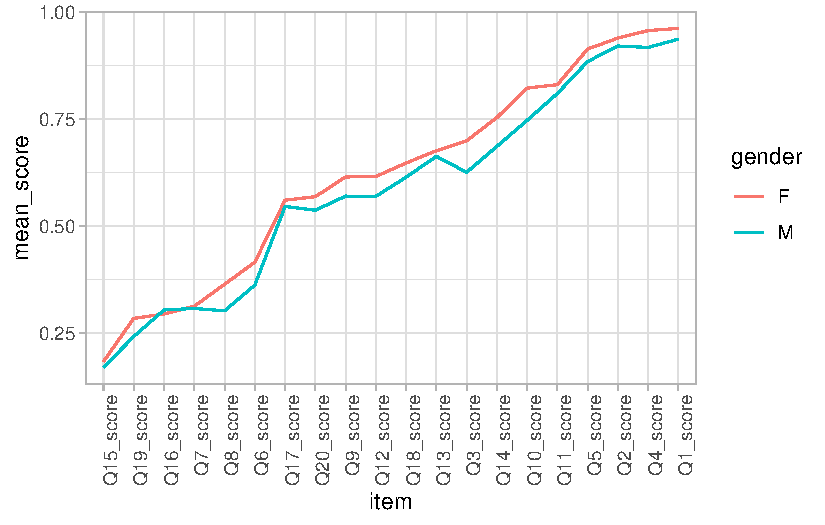
\includegraphics{ct-dif_files/figure-pdf/unnamed-chunk-6-1.pdf}

}

\end{figure}

\part{The Rasch Model}

\hypertarget{rasch-measurement}{%
\chapter{Rasch Measurement}\label{rasch-measurement}}

Rasch measurement theory is a method for transforming data from
multiple-choice tests, surveys, or other assessments into a scale that
reflects a person's level of understanding or skill. The theory is based
on the idea of invariance in measurement, which means that the
comparison between two stimuli or individuals should be independent of
who was involved in the comparison.

Rasch models are used to identify deviations from the model's
requirements when they occur. These deviations can help researchers
identify areas for additional research or guide improvements in the
quality of the assessment procedure.

Rasch models have several theoretical and practical features that make
them popular across disciplines in the social, behavioral, and health
sciences.

Wright and Mok (2004) summarized the key theoretical and practical
features of the Rasch measurement approach as follows:

In order to construct inference from observation, the measurement model
must: (a) produce linear measures (b) overcome missing data (c) give
estimates of precision (d) have devices for detecting misfit (e) the
parameters of the object being measured and of the measurement
instrument must be separable.

Only the family of Rasch measurement models solve these problems. (p.~4)

Wright, Benjamin D., and Magdalena Mo Ching Mok. An overview of the
family of Rasch measurement models. In E. V. Smith \& R. M. Smith
(Eds.), Introduction to Rasch Measurement, JAM Press, 2004, 1--24.

\hypertarget{some-introductory-texts}{%
\section{Some introductory texts}\label{some-introductory-texts}}

Andrich, David, and Ida Marais. A Course in Rasch Measurement Theory:
Measuring in the Educational, Social and Health Sciences. Singapore:
Springer, 2019.

Bond, Trevor G., Zi Yan, and Moritz Heene. Applying the Rasch Model:
Fundamental Measurement in the Human Sciences (4th Ed.). New York:
Routledge, Taylor \& Francis Group, 2020.

Engelhard, Georg, and Jue Wang. Rasch Models for solving measurement
problems: Invariant Measurement in the Social Sciences. Vol.187. SAGE,
2020.
https://us.sagepub.com/en-us/nam/rasch-models-for-solving-measurement-problems/book267292

\hypertarget{rasch-controversies}{%
\section{Rasch controversies}\label{rasch-controversies}}

There have been some controversies surrounding the use of the Rasch
model in educational and social science research. Here are some of the
main points of debate:

\hypertarget{assumption-of-unidimensionality}{%
\subsection{Assumption of
unidimensionality}\label{assumption-of-unidimensionality}}

The Rasch model assumes that the underlying construct being measured is
unidimensional, meaning that all of the items in the test are measuring
the same thing. Critics argue that this assumption is often violated in
practice, particularly in complex constructs such as reading
comprehension or mathematical ability.

\hypertarget{lack-of-fit-to-the-model}{%
\subsection{Lack of fit to the model}\label{lack-of-fit-to-the-model}}

While the Rasch model provides a good fit for many datasets, it is not
always an accurate representation of the underlying data. Researchers
have proposed alternative models, such as multidimensional item response
theory (MIRT), to account for the complexity and multidimensionality of
constructs.

\hypertarget{lack-of-flexibility}{%
\subsection{Lack of flexibility}\label{lack-of-flexibility}}

The Rasch model is relatively inflexible and cannot accommodate certain
types of data, such as data that violates the assumption of local
independence (meaning that responses to one item may depend on responses
to another item). Alternative models, such as the partial credit model
or the generalized partial credit model, have been proposed to address
these limitations.

\hypertarget{interpretation-of-scores}{%
\subsection{Interpretation of scores}\label{interpretation-of-scores}}

While Rasch scores are often interpreted as linear measures of a
person's ability or level of understanding, critics argue that this
interpretation may not always be appropriate, particularly if the
construct being measured is not unidimensional or if the Rasch model
does not provide a good fit to the data.

\hypertarget{rasch-wars}{%
\section{Rasch Wars!}\label{rasch-wars}}

Panayides, P., Robinson, C. and Tymms, P. (2010), The assessment
revolution that has passed England by: Rasch measurement. British
Educational Research Journal, 36: 611-626.
\url{https://doi.org/10.1080/01411920903018182} Goldstein, H. and
Blinkhorn, S. (1982), The Rasch Model Still Does Not Fit. British
Educational Research Journal, 8: 167-170.
\url{https://doi.org/10.1080/0141192820080207}

\hypertarget{item-response-theory}{%
\chapter{Item Response Theory}\label{item-response-theory}}

Item Response Theory (IRT) uses a mathematical function to model the
probability of a person's success on a test item, given their level of
ability and the item's difficulty. The function should be bounded by 0
and 1, meaning that it models probability. It should also be increasing,
indicating that the chance of success is higher for people with higher
abilities. The function should have an S-shaped curve, with the left
side close to 0 and the right side close to 1 but not exceeding it.

There are several mathematical functions that fit this shape, such as
cumulative distribution functions (cdf) or ogives. Examples of ogives
that have been used in IRT include the logistic ogive and the normal
ogive, but for the purposes of this discussion, we will focus on the
logistic ogive. The logistic ogive is a function that can be used to
model the probability of success on an item and has the desired S-shaped
curve, making it a commonly used function in IRT.

The Rasch item response model (Rasch 1960) uses the following function
to model the probability of success on an item with item difficulty δ
and ability θ

\[
Prob(X=1) = \frac{\exp(\theta - \delta)}{1+\exp(\theta - \delta)}
\]

where \emph{X} is the person's score on the item, taking values of 0 or
1.

\begin{Shaded}
\begin{Highlighting}[]
\CommentTok{\# Calculate Rasch model probability}
\NormalTok{delta }\OtherTok{\textless{}{-}} \FloatTok{0.6}  \CommentTok{\#item difficulty is 0.6}
\NormalTok{theta }\OtherTok{\textless{}{-}} \FloatTok{1.0}  \CommentTok{\#person ability is 1.0}
\NormalTok{prob }\OtherTok{\textless{}{-}} \FunctionTok{exp}\NormalTok{(theta}\SpecialCharTok{{-}}\NormalTok{delta)}\SpecialCharTok{/}\NormalTok{(}\DecValTok{1}\SpecialCharTok{+}\FunctionTok{exp}\NormalTok{(theta}\SpecialCharTok{{-}}\NormalTok{delta))}
\NormalTok{prob}
\end{Highlighting}
\end{Shaded}

\begin{verbatim}
[1] 0.5986877
\end{verbatim}

Change the values of delta and theta, and observe how prob changes. In
particular, try values when (1) delta = theta, (2) delta \textgreater{}
theta, and (3) delta \textless{} theta. What happens when theta is very
high, and when theta is very low?

We will plot the probability as a function of θ.

\begin{Shaded}
\begin{Highlighting}[]
\CommentTok{\#Calculate prob as a function the theta}
\NormalTok{id }\OtherTok{=} \DecValTok{1} \CommentTok{\# item id}
\NormalTok{delta }\OtherTok{\textless{}{-}} \DecValTok{1} \CommentTok{\#item difficulty is 1}
\NormalTok{theta }\OtherTok{\textless{}{-}} \FunctionTok{seq}\NormalTok{(}\SpecialCharTok{{-}}\DecValTok{3}\NormalTok{,}\DecValTok{3}\NormalTok{,}\FloatTok{0.01}\NormalTok{) }\CommentTok{\#a vector of theta from {-}3 to 3 in steps of 0.01}
\NormalTok{prob\_function }\OtherTok{\textless{}{-}} \ControlFlowTok{function}\NormalTok{(theta, delta)\{}
    \FunctionTok{return}\NormalTok{ (}\FunctionTok{exp}\NormalTok{(theta}\SpecialCharTok{{-}}\NormalTok{delta)}\SpecialCharTok{/}\NormalTok{(}\DecValTok{1}\SpecialCharTok{+}\FunctionTok{exp}\NormalTok{(theta}\SpecialCharTok{{-}}\NormalTok{delta)))}
\NormalTok{\}}

\NormalTok{probs }\OtherTok{\textless{}{-}} \FunctionTok{tibble}\NormalTok{(}\AttributeTok{id =}\NormalTok{ id, }\AttributeTok{delta=}\NormalTok{delta,}\AttributeTok{theta=}\NormalTok{theta)}
\NormalTok{probs }\OtherTok{\textless{}{-}}\NormalTok{ probs }\SpecialCharTok{\%\textgreater{}\%} \FunctionTok{mutate}\NormalTok{(}\AttributeTok{prob =} \FunctionTok{prob\_function}\NormalTok{(theta, delta))}

\NormalTok{p }\OtherTok{\textless{}{-}} \FunctionTok{ggplot}\NormalTok{(probs, }\FunctionTok{aes}\NormalTok{(}\AttributeTok{x=}\NormalTok{theta, }\AttributeTok{y=}\NormalTok{prob))}
\NormalTok{p }\OtherTok{\textless{}{-}}\NormalTok{ p }\SpecialCharTok{+} \FunctionTok{geom\_line}\NormalTok{()}
\FunctionTok{print}\NormalTok{(p)}
\end{Highlighting}
\end{Shaded}

\begin{figure}[H]

{\centering 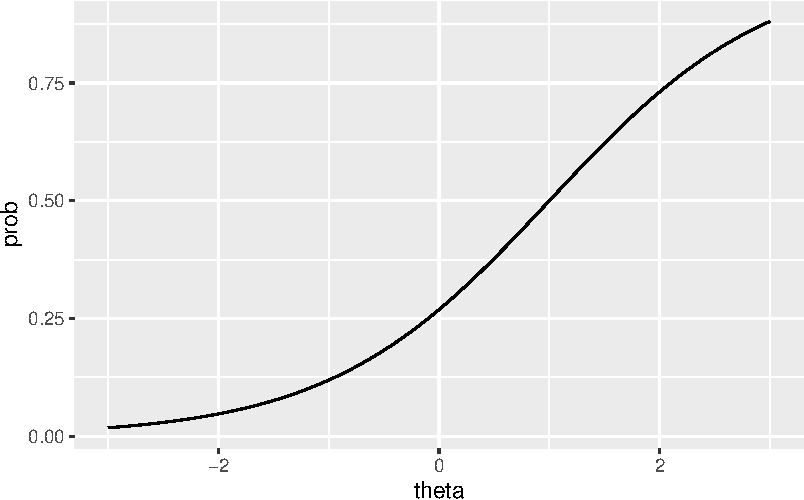
\includegraphics{rasch-2_files/figure-pdf/fig-item-cc-1.pdf}

}

\caption{\label{fig-item-cc}Item Characteristic Curve}

\end{figure}

\hypertarget{exercise}{%
\section{Exercise}\label{exercise}}

As an exercise, plot three ICC for three items with (1) δ = −1, (2) δ =
0, and (3) δ = 1.

See if you can work out how to plot the three graphs using different
colors. Can you easily identify the ICC of the easier item?

\hypertarget{theta-scale-unit}{%
\section{Theta Scale Unit}\label{theta-scale-unit}}

The θ scale is in ``logit'' unit. Answer the following questions,
assuming the item responses follow a Rasch model:

\begin{enumerate}
\def\labelenumi{\arabic{enumi}.}
\tightlist
\item
  What is the probability of success when θ = δ?
\item
  What is the probability of success when θ = 2 logit and δ = 1 logit?
\item
  What is the probability of success when a person's ability is 1.5
  logit higher than the item difficulty?
\item
  What is the probability of success when a person's ability is 0.6
  logit lower than the item difficulty?
\item
  Is the following statement TRUE or FALSE: The difference in logit
  between a person's ability and an item's difficulty determines the
  probability of success, irrespective of what the ability is.
\item
  Consider CTT item difficulty and person ability, can we say anything
  about the likelihood of success for a person who scored 80\% on a
  test, on an item where 80\% of the candidates answered correctly?
\end{enumerate}

\hypertarget{two-parameter-irt-model}{%
\chapter{Two-parameter IRT model}\label{two-parameter-irt-model}}

Mathematically, the two-parameter IRT model has a discrimination
parameter in addition to the item difficulty parameter.

\[
Prob(X=1) = \frac{\exp(a(\theta - \delta))}{1+\exp(a(\theta - \delta))}
\]

where \emph{a} is called the discrimination parameter.

The result of including a discrimination parameter is that the slopes of
the Item Characteristic Curves are no longer parallel.

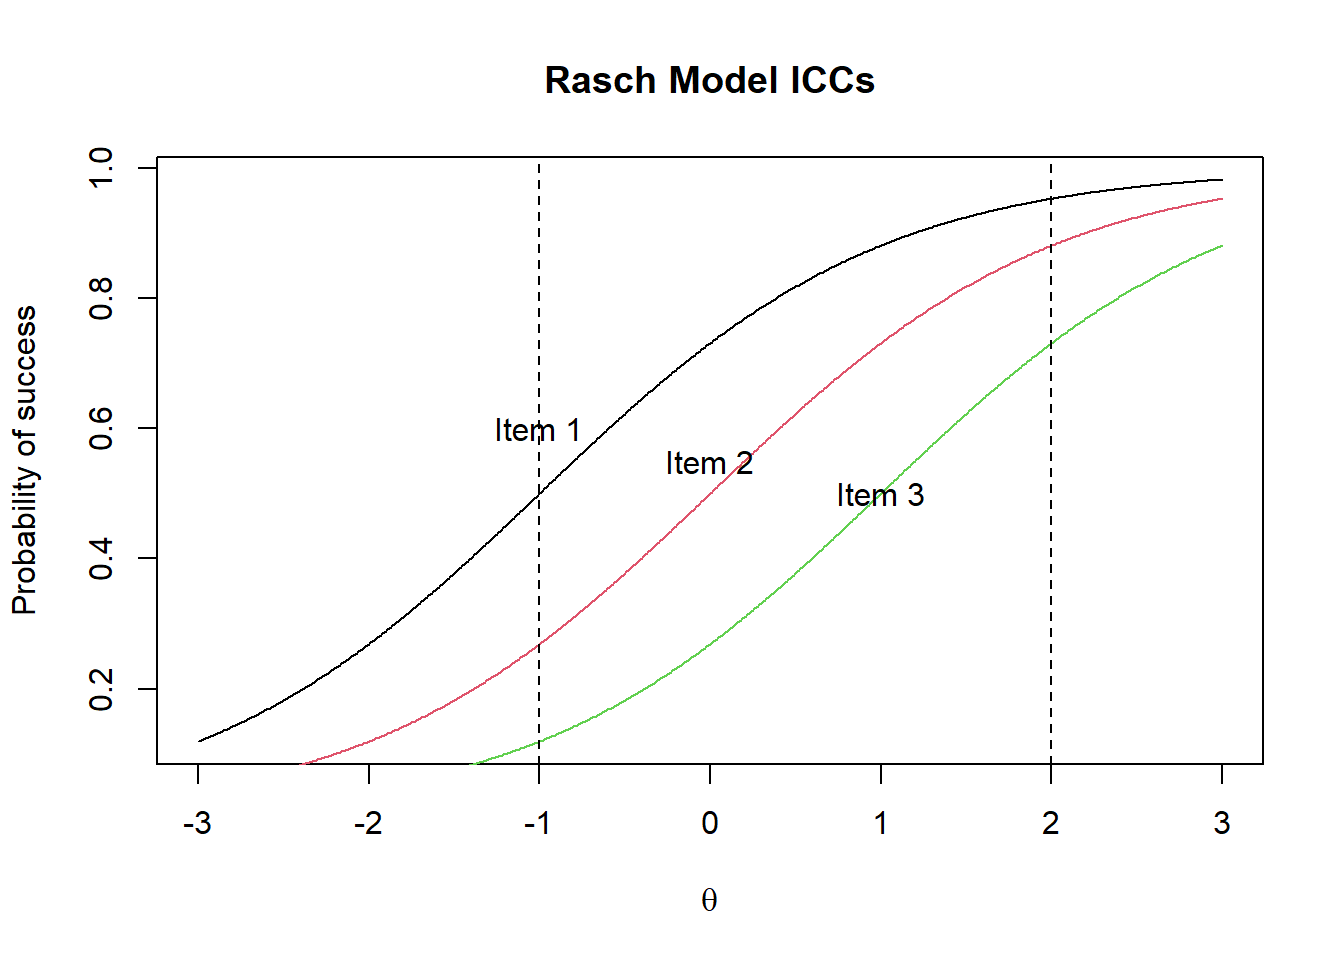
\includegraphics{images/ICC2-1.png} 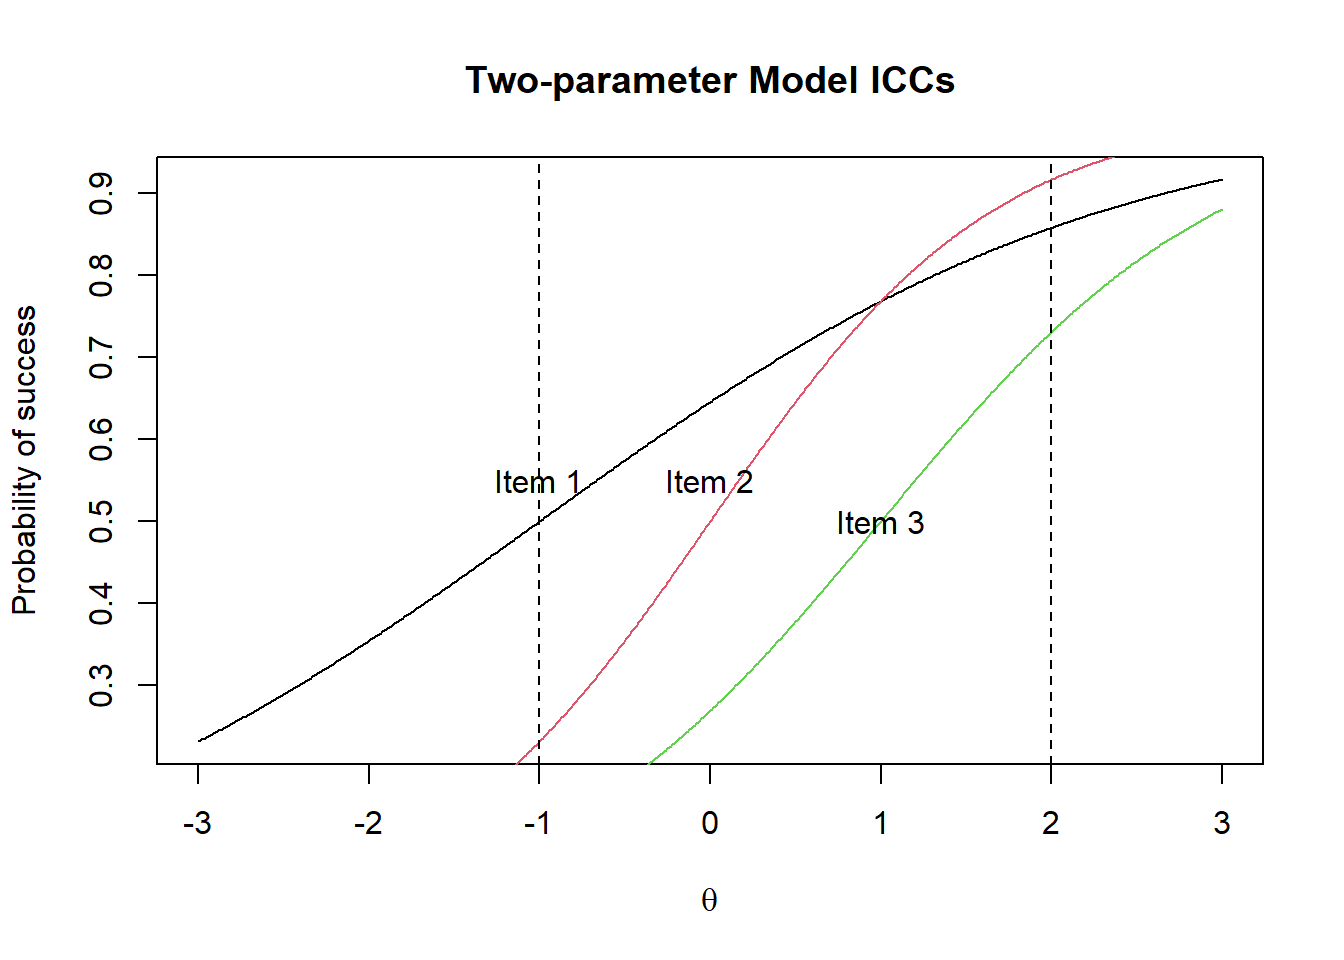
\includegraphics{images/ICC3-1.png}

Under the Rasch model, for any person, Item 1 is easier than Item 2
which is easier than item 3.

Under the two-parameter IRT model ICCs are not parallel. For a person
with ability measure of -1 logit, Item 1 is the easiest item. But for a
person with an ability of 2 logits, Item 2 is the easiest item.

\hypertarget{exercise-1}{%
\section{Exercise}\label{exercise-1}}

Amend the equation for the Rasch model so that it now has a
discrimination parameter. Plot ICCs with different discrimination
parameters to see the impact of manipulating alpha.

\begin{Shaded}
\begin{Highlighting}[]
\CommentTok{\#Calculate prob as a function the theta}
\NormalTok{id }\OtherTok{=} \DecValTok{1} \CommentTok{\# item id}
\NormalTok{delta }\OtherTok{\textless{}{-}} \DecValTok{1} \CommentTok{\#item difficulty is 1}
\NormalTok{theta }\OtherTok{\textless{}{-}} \FunctionTok{seq}\NormalTok{(}\SpecialCharTok{{-}}\DecValTok{3}\NormalTok{,}\DecValTok{3}\NormalTok{,}\FloatTok{0.01}\NormalTok{) }\CommentTok{\#a vector of theta from {-}3 to 3 in steps of 0.01}
\NormalTok{irt\_function }\OtherTok{\textless{}{-}} \ControlFlowTok{function}\NormalTok{(alpha, theta, delta)\{}
    
\NormalTok{\}}
\end{Highlighting}
\end{Shaded}

\hypertarget{discussion-1}{%
\section{Discussion}\label{discussion-1}}

Play the scoring game:

\url{https://dexter-psychometrics.github.io/dexter/articles/blog/2018-09-24-the-scoring-game}

How do you feel about using the 2PL model to score a high stakes
examination?

Now read on \ldots{}

\url{https://dexter-psychometrics.github.io/dexter/articles/blog/2022-06-20-Woes_with_2PL}

\hypertarget{assessing-the-fit-of-the-rasch-model}{%
\chapter{Assessing the fit of the Rasch
model}\label{assessing-the-fit-of-the-rasch-model}}

\hypertarget{how-does-rasch-differ-from-regression-models}{%
\section{How does Rasch differ from regression
models?}\label{how-does-rasch-differ-from-regression-models}}

\url{https://dexter-psychometrics.github.io/dexter/articles/blog/2018-02-25-item-total-regressions-in-dexter}

\begin{Shaded}
\begin{Highlighting}[]
\FunctionTok{rm}\NormalTok{(}\AttributeTok{list=}\FunctionTok{ls}\NormalTok{())}
\FunctionTok{library}\NormalTok{(tidyverse)}
\FunctionTok{library}\NormalTok{(dexter)}
\CommentTok{\# load in the dataset}
\NormalTok{responses }\OtherTok{\textless{}{-}} \FunctionTok{read\_csv}\NormalTok{(}\StringTok{\textquotesingle{}data/responses.csv\textquotesingle{}}\NormalTok{)}
\NormalTok{keys }\OtherTok{\textless{}{-}} \FunctionTok{read\_csv}\NormalTok{(}\StringTok{\textquotesingle{}data/key.csv\textquotesingle{}}\NormalTok{)}
\CommentTok{\# Create the rules}
\NormalTok{rules }\OtherTok{\textless{}{-}} \FunctionTok{keys\_to\_rules}\NormalTok{(keys, }\AttributeTok{include\_NA\_rule =} \ConstantTok{TRUE}\NormalTok{)}
\NormalTok{db }\OtherTok{\textless{}{-}} \FunctionTok{start\_new\_project}\NormalTok{(rules, }\AttributeTok{db\_name =} \StringTok{":memory:"}\NormalTok{, }\AttributeTok{person\_properties=}\FunctionTok{list}\NormalTok{(}\AttributeTok{gender=}\StringTok{"unknown"}\NormalTok{))}
\end{Highlighting}
\end{Shaded}

\hypertarget{fitting-the-rasch-model}{%
\section{Fitting the Rasch model}\label{fitting-the-rasch-model}}

Look at Item Characteristic Plots for all items. There are three
item-test regressions on the plot: the observed one, shown as pink dots;
the interaction model, shown with a thick gray line; and the ENORM
model, shown with a thin black line. (ENORM=RASCH for dichotomous
models)

\begin{Shaded}
\begin{Highlighting}[]
\FunctionTok{add\_booklet}\NormalTok{(db, responses, }\StringTok{"y7"}\NormalTok{) }
\end{Highlighting}
\end{Shaded}

\begin{verbatim}
no column `person_id` provided, automatically generating unique person id's
\end{verbatim}

\begin{verbatim}
$items
 [1] "Q1"  "Q2"  "Q3"  "Q4"  "Q5"  "Q6"  "Q7"  "Q8"  "Q9"  "Q10" "Q11" "Q12"
[13] "Q13" "Q14" "Q15" "Q16" "Q17" "Q18" "Q19" "Q20"

$person_properties
[1] "gender"

$columns_ignored
 [1] "id"        "dob"       "yg"        "missing"   "Q1_score"  "Q2_score" 
 [7] "Q3_score"  "Q4_score"  "Q5_score"  "Q6_score"  "Q7_score"  "Q8_score" 
[13] "Q9_score"  "Q10_score" "Q11_score" "Q12_score" "Q13_score" "Q14_score"
[19] "Q15_score" "Q16_score" "Q17_score" "Q18_score" "Q19_score" "Q20_score"
\end{verbatim}

\begin{Shaded}
\begin{Highlighting}[]
\FunctionTok{get\_booklets}\NormalTok{(db)}
\end{Highlighting}
\end{Shaded}

\begin{verbatim}
  booklet_id n_items n_persons booklet_max_score
1         y7      20      3061                20
\end{verbatim}

\begin{Shaded}
\begin{Highlighting}[]
\NormalTok{m }\OtherTok{=} \FunctionTok{fit\_inter}\NormalTok{(db, booklet\_id}\SpecialCharTok{==}\StringTok{\textquotesingle{}y7\textquotesingle{}}\NormalTok{)}

\NormalTok{n\_items }\OtherTok{\textless{}{-}} \FunctionTok{nrow}\NormalTok{(keys)}
\ControlFlowTok{for}\NormalTok{(i }\ControlFlowTok{in} \DecValTok{1}\SpecialCharTok{:}\NormalTok{n\_items)\{}
  \FunctionTok{plot}\NormalTok{(m, keys}\SpecialCharTok{$}\NormalTok{item\_id[i], }\AttributeTok{show.observed=}\ConstantTok{TRUE}\NormalTok{)}
\NormalTok{\}}
\end{Highlighting}
\end{Shaded}

\begin{figure}[H]

{\centering 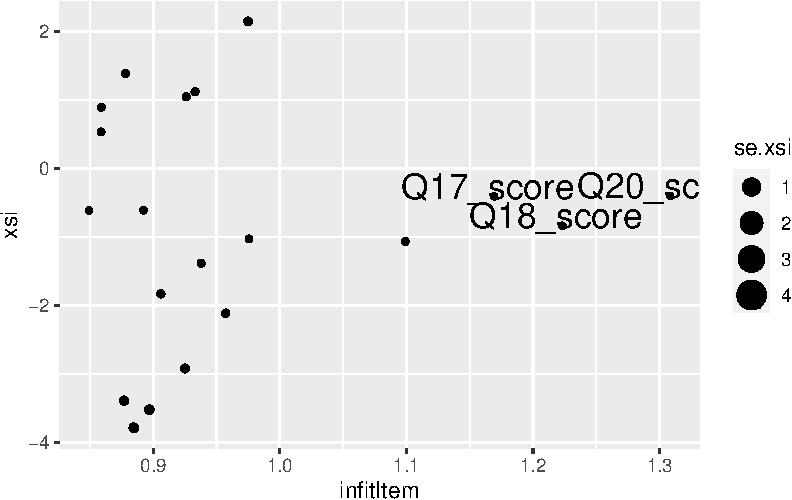
\includegraphics{rasch-regression_files/figure-pdf/unnamed-chunk-2-1.pdf}

}

\end{figure}

\begin{figure}[H]

{\centering 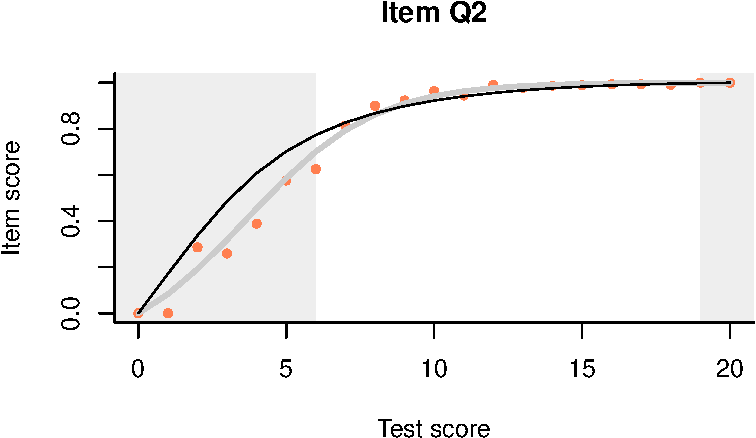
\includegraphics{rasch-regression_files/figure-pdf/unnamed-chunk-2-2.pdf}

}

\end{figure}

\begin{figure}[H]

{\centering 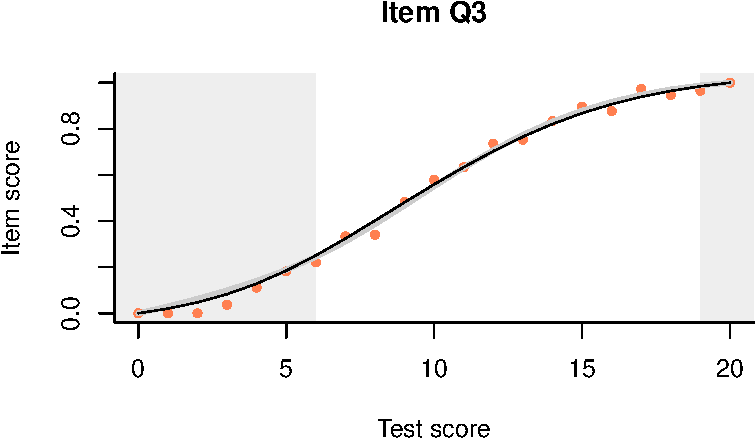
\includegraphics{rasch-regression_files/figure-pdf/unnamed-chunk-2-3.pdf}

}

\end{figure}

\begin{figure}[H]

{\centering 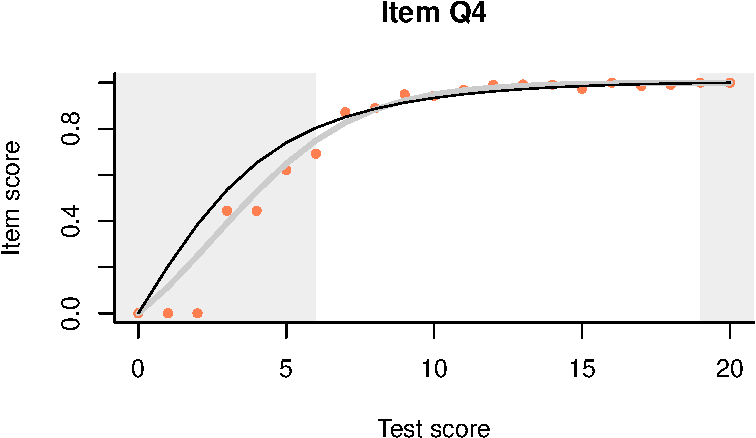
\includegraphics{rasch-regression_files/figure-pdf/unnamed-chunk-2-4.pdf}

}

\end{figure}

\begin{figure}[H]

{\centering 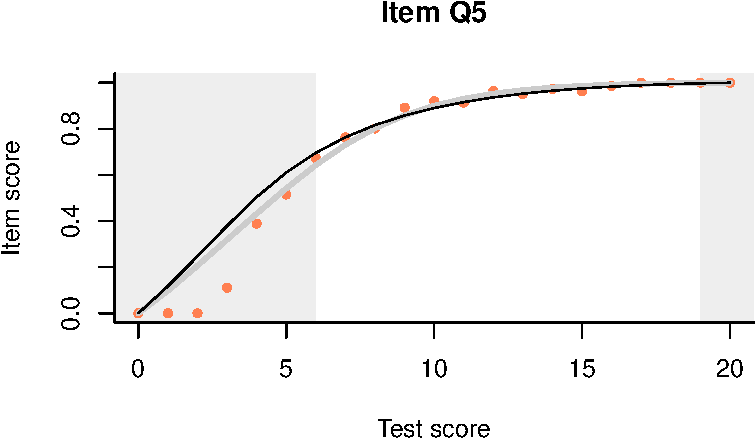
\includegraphics{rasch-regression_files/figure-pdf/unnamed-chunk-2-5.pdf}

}

\end{figure}

\begin{figure}[H]

{\centering 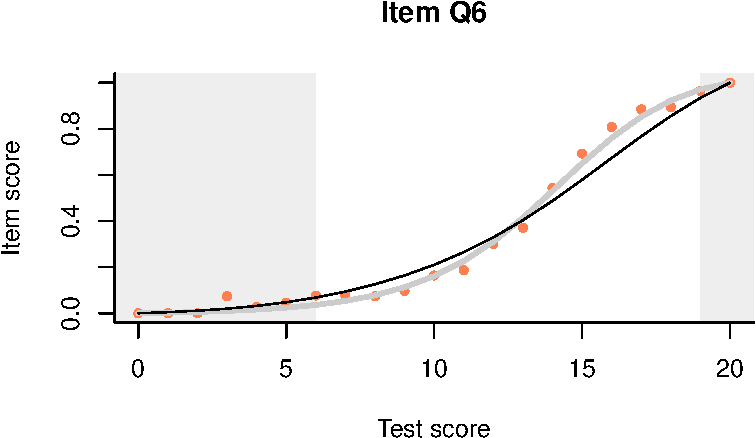
\includegraphics{rasch-regression_files/figure-pdf/unnamed-chunk-2-6.pdf}

}

\end{figure}

\begin{figure}[H]

{\centering 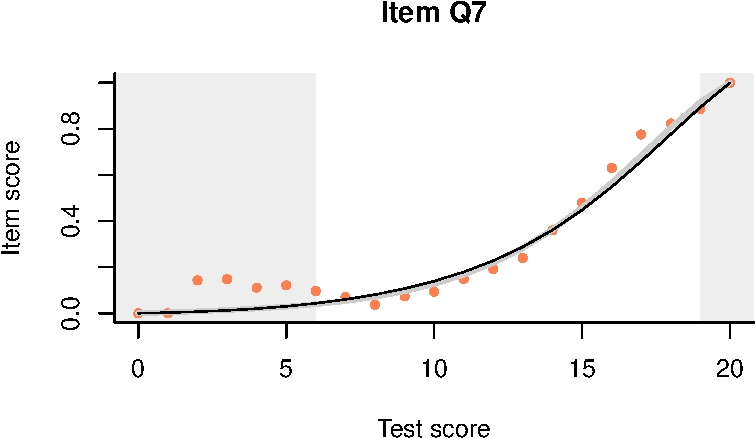
\includegraphics{rasch-regression_files/figure-pdf/unnamed-chunk-2-7.pdf}

}

\end{figure}

\begin{figure}[H]

{\centering 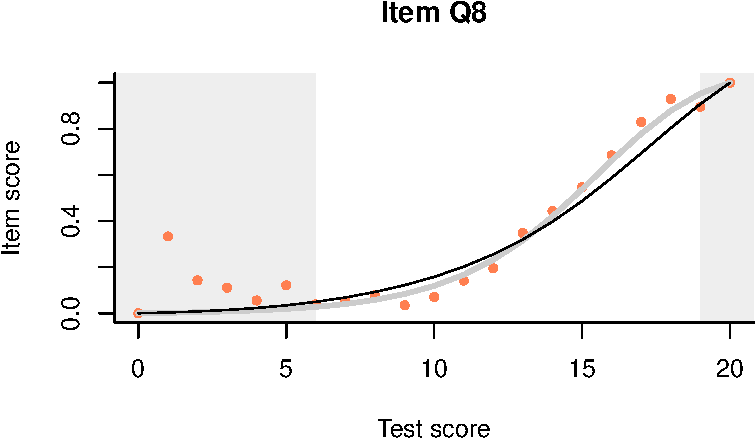
\includegraphics{rasch-regression_files/figure-pdf/unnamed-chunk-2-8.pdf}

}

\end{figure}

\begin{figure}[H]

{\centering 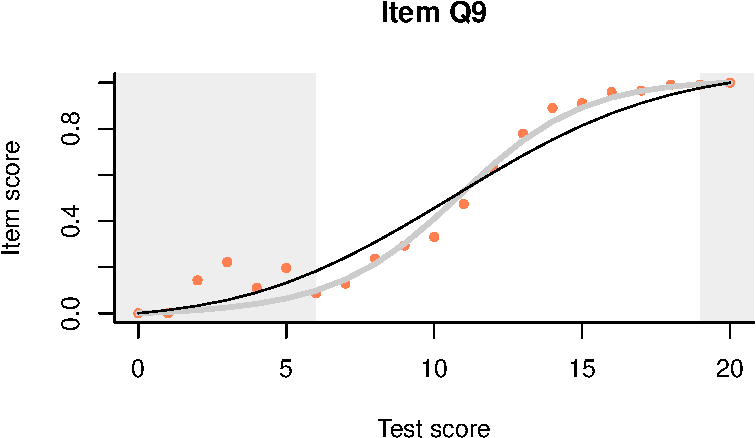
\includegraphics{rasch-regression_files/figure-pdf/unnamed-chunk-2-9.pdf}

}

\end{figure}

\begin{figure}[H]

{\centering 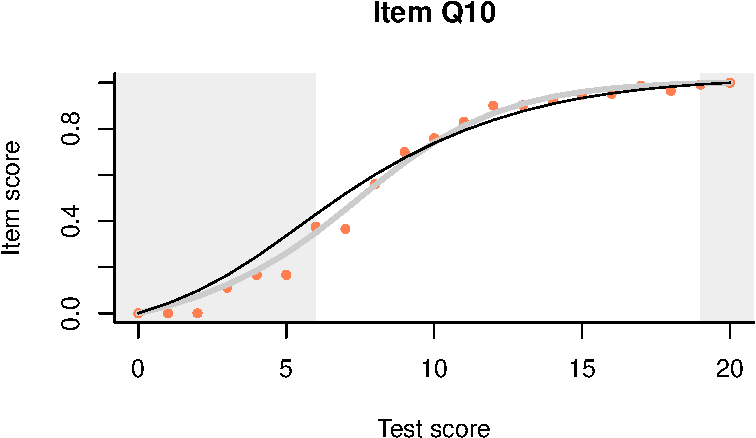
\includegraphics{rasch-regression_files/figure-pdf/unnamed-chunk-2-10.pdf}

}

\end{figure}

\begin{figure}[H]

{\centering 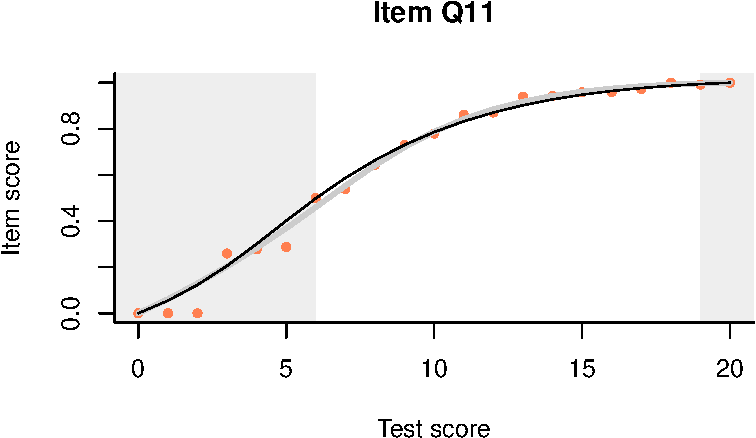
\includegraphics{rasch-regression_files/figure-pdf/unnamed-chunk-2-11.pdf}

}

\end{figure}

\begin{figure}[H]

{\centering 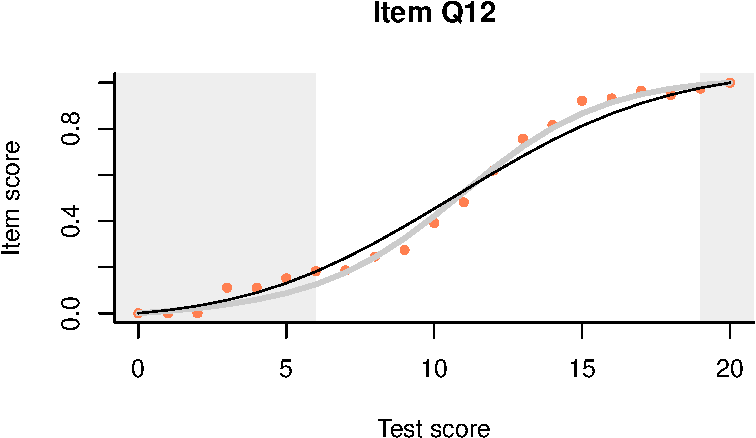
\includegraphics{rasch-regression_files/figure-pdf/unnamed-chunk-2-12.pdf}

}

\end{figure}

\begin{figure}[H]

{\centering 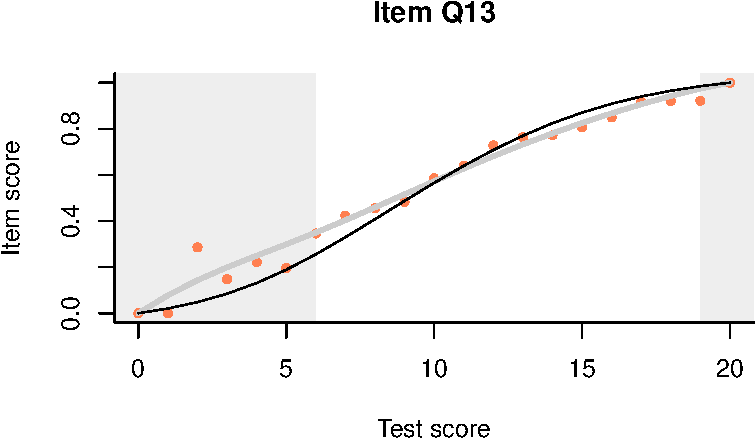
\includegraphics{rasch-regression_files/figure-pdf/unnamed-chunk-2-13.pdf}

}

\end{figure}

\begin{figure}[H]

{\centering 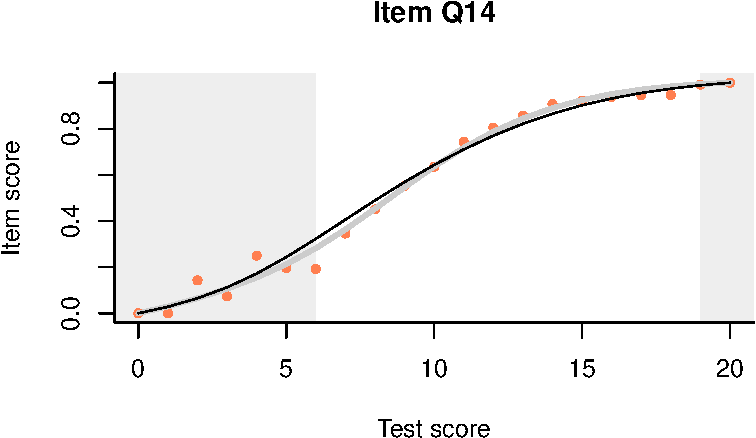
\includegraphics{rasch-regression_files/figure-pdf/unnamed-chunk-2-14.pdf}

}

\end{figure}

\begin{figure}[H]

{\centering 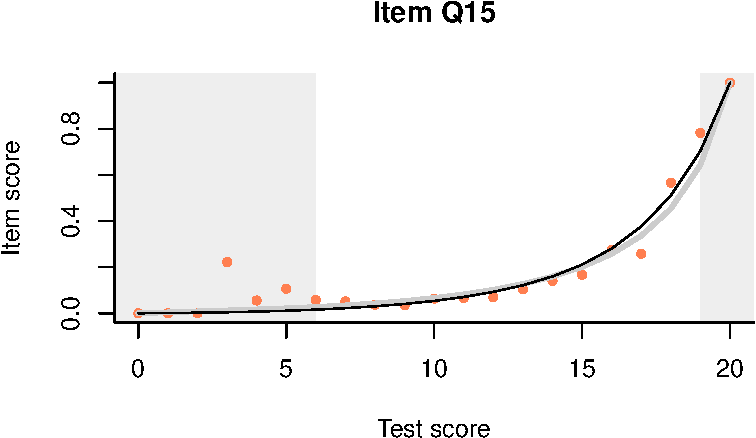
\includegraphics{rasch-regression_files/figure-pdf/unnamed-chunk-2-15.pdf}

}

\end{figure}

\begin{figure}[H]

{\centering 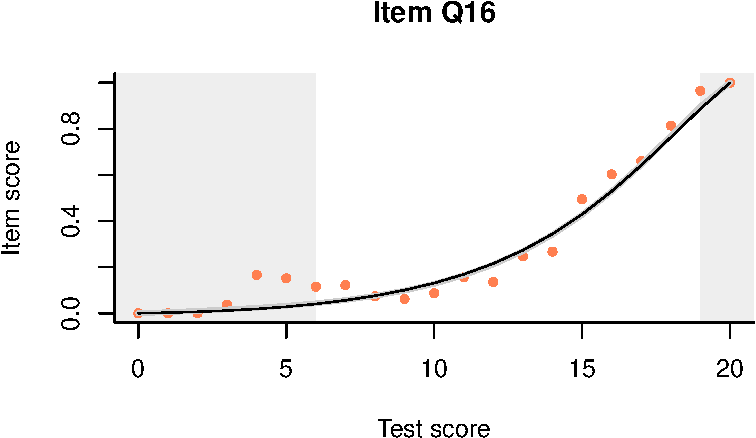
\includegraphics{rasch-regression_files/figure-pdf/unnamed-chunk-2-16.pdf}

}

\end{figure}

\begin{figure}[H]

{\centering 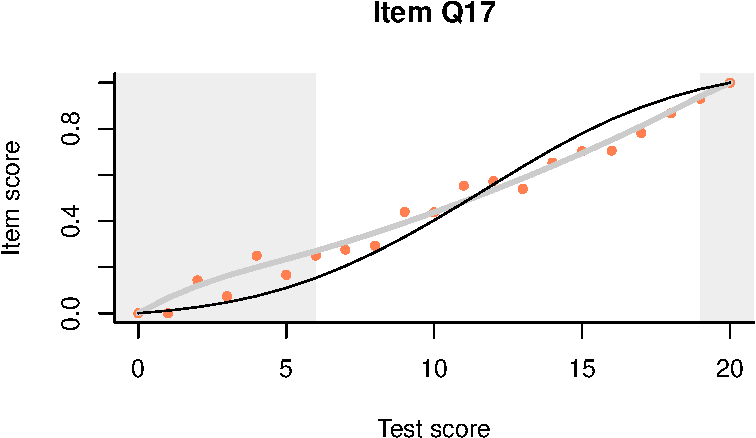
\includegraphics{rasch-regression_files/figure-pdf/unnamed-chunk-2-17.pdf}

}

\end{figure}

\begin{figure}[H]

{\centering 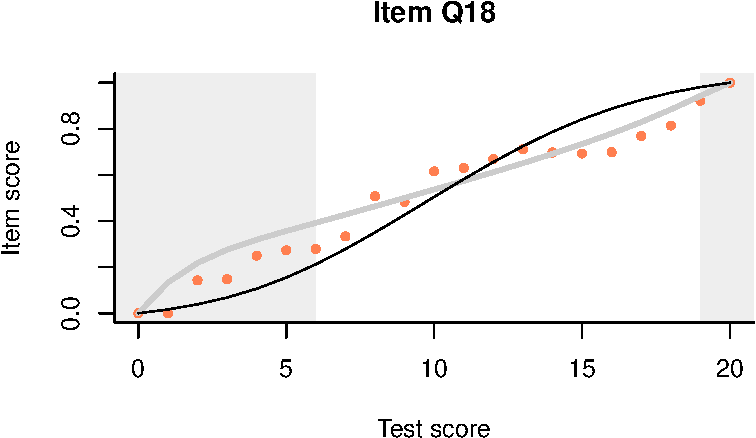
\includegraphics{rasch-regression_files/figure-pdf/unnamed-chunk-2-18.pdf}

}

\end{figure}

\begin{figure}[H]

{\centering \includegraphics{rasch-regression_files/figure-pdf/unnamed-chunk-2-19.pdf}

}

\end{figure}

\begin{figure}[H]

{\centering \includegraphics{rasch-regression_files/figure-pdf/unnamed-chunk-2-20.pdf}

}

\end{figure}

\begin{Shaded}
\begin{Highlighting}[]
\NormalTok{tt }\OtherTok{=} \FunctionTok{tia\_tables}\NormalTok{(db)}
\NormalTok{knitr}\SpecialCharTok{::}\FunctionTok{kable}\NormalTok{(tt}\SpecialCharTok{$}\NormalTok{items)}
\end{Highlighting}
\end{Shaded}

\begin{longtable}[]{@{}
  >{\raggedright\arraybackslash}p{(\columnwidth - 16\tabcolsep) * \real{0.1222}}
  >{\raggedright\arraybackslash}p{(\columnwidth - 16\tabcolsep) * \real{0.0889}}
  >{\raggedleft\arraybackslash}p{(\columnwidth - 16\tabcolsep) * \real{0.1222}}
  >{\raggedleft\arraybackslash}p{(\columnwidth - 16\tabcolsep) * \real{0.1111}}
  >{\raggedleft\arraybackslash}p{(\columnwidth - 16\tabcolsep) * \real{0.1111}}
  >{\raggedleft\arraybackslash}p{(\columnwidth - 16\tabcolsep) * \real{0.1111}}
  >{\raggedleft\arraybackslash}p{(\columnwidth - 16\tabcolsep) * \real{0.1111}}
  >{\raggedleft\arraybackslash}p{(\columnwidth - 16\tabcolsep) * \real{0.1111}}
  >{\raggedleft\arraybackslash}p{(\columnwidth - 16\tabcolsep) * \real{0.1111}}@{}}
\toprule\noalign{}
\begin{minipage}[b]{\linewidth}\raggedright
booklet\_id
\end{minipage} & \begin{minipage}[b]{\linewidth}\raggedright
item\_id
\end{minipage} & \begin{minipage}[b]{\linewidth}\raggedleft
mean\_score
\end{minipage} & \begin{minipage}[b]{\linewidth}\raggedleft
sd\_score
\end{minipage} & \begin{minipage}[b]{\linewidth}\raggedleft
max\_score
\end{minipage} & \begin{minipage}[b]{\linewidth}\raggedleft
pvalue
\end{minipage} & \begin{minipage}[b]{\linewidth}\raggedleft
rit
\end{minipage} & \begin{minipage}[b]{\linewidth}\raggedleft
rir
\end{minipage} & \begin{minipage}[b]{\linewidth}\raggedleft
n\_persons
\end{minipage} \\
\midrule\noalign{}
\endhead
\bottomrule\noalign{}
\endlastfoot
y7 & Q1 & 0.9460960 & 0.2258281 & 1 & 0.9460960 & 0.3334998 & 0.2822894
& 3061 \\
y7 & Q10 & 0.7817707 & 0.4130439 & 1 & 0.7817707 & 0.4890928 & 0.4051286
& 3061 \\
y7 & Q11 & 0.8160732 & 0.3874245 & 1 & 0.8160732 & 0.4369315 & 0.3542171
& 3061 \\
y7 & Q12 & 0.5870631 & 0.4923617 & 1 & 0.5870631 & 0.5774198 & 0.4869096
& 3061 \\
y7 & Q13 & 0.6644887 & 0.4721689 & 1 & 0.6644887 & 0.4167201 & 0.3128742
& 3061 \\
y7 & Q14 & 0.7170859 & 0.4504150 & 1 & 0.7170859 & 0.5027417 & 0.4120081
& 3061 \\
y7 & Q15 & 0.1754329 & 0.3803369 & 1 & 0.1754329 & 0.4521971 & 0.3722567
& 3061 \\
y7 & Q16 & 0.2969618 & 0.4569196 & 1 & 0.2969618 & 0.5363749 & 0.4479760
& 3061 \\
y7 & Q17 & 0.5508004 & 0.4974126 & 1 & 0.5508004 & 0.4103008 & 0.2999650
& 3061 \\
y7 & Q18 & 0.6229990 & 0.4846352 & 1 & 0.6229990 & 0.3456235 & 0.2334171
& 3061 \\
y7 & Q19 & 0.2606991 & 0.4390160 & 1 & 0.2606991 & 0.5611054 & 0.4793179
& 3061 \\
y7 & Q2 & 0.9235544 & 0.2657098 & 1 & 0.9235544 & 0.3706761 & 0.3117073
& 3061 \\
y7 & Q20 & 0.5485136 & 0.4976409 & 1 & 0.5485136 & 0.3256473 & 0.2089781
& 3061 \\
y7 & Q3 & 0.6602418 & 0.4736270 & 1 & 0.6602418 & 0.5033116 & 0.4075765
& 3061 \\
y7 & Q4 & 0.9340085 & 0.2482672 & 1 & 0.9340085 & 0.3441510 & 0.2881099
& 3061 \\
y7 & Q5 & 0.8961124 & 0.3051147 & 1 & 0.8961124 & 0.3780087 & 0.3103319
& 3061 \\
y7 & Q6 & 0.3868017 & 0.4870176 & 1 & 0.3868017 & 0.6149106 & 0.5308310
& 3061 \\
y7 & Q7 & 0.3074159 & 0.4614232 & 1 & 0.3074159 & 0.5552584 & 0.4681820
& 3061 \\
y7 & Q8 & 0.3299575 & 0.4701974 & 1 & 0.3299575 & 0.6029375 & 0.5203720
& 3061 \\
y7 & Q9 & 0.5890232 & 0.4920110 & 1 & 0.5890232 & 0.6062016 & 0.5198674
& 3061 \\
\end{longtable}

\hypertarget{analysis}{%
\section{Analysis}\label{analysis}}

\hypertarget{guessing}{%
\subsection{Guessing}\label{guessing}}

The left hand curtain gives us an idea of guessing. By default, they are
drawn at the 5th and the 95th percentile of the observed test scores,
highlighting the central 90\% of the data. The left curtain highlights
the likely item score for the pupils at the 95th percentile. From
examination of the ICCs, which items are prone to guessing?

\hypertarget{model-fit}{%
\subsection{Model fit}\label{model-fit}}

Which items seem to fit the Rasch model less well? Which restriction of
the Rasch model do these items highlight? How can the fit of the model
be improved?

\begin{Shaded}
\begin{Highlighting}[]
\FunctionTok{close\_project}\NormalTok{(db)}
\end{Highlighting}
\end{Shaded}

\hypertarget{item-difficulty-and-person-ability}{%
\chapter{Item Difficulty and Person
Ability}\label{item-difficulty-and-person-ability}}

\hypertarget{fitting-the-rasch-model-with-tam}{%
\section{Fitting the Rasch model with
TAM}\label{fitting-the-rasch-model-with-tam}}

\begin{Shaded}
\begin{Highlighting}[]
\FunctionTok{rm}\NormalTok{(}\AttributeTok{list=}\FunctionTok{ls}\NormalTok{())  }\CommentTok{\#remove all variables in the R environment}
\FunctionTok{library}\NormalTok{(tidyverse)}
\FunctionTok{library}\NormalTok{(TAM)  }\CommentTok{\#load the package TAM so we can use the functions in TAM}

\CommentTok{\# load in the dataset}
\NormalTok{responses }\OtherTok{\textless{}{-}} \FunctionTok{read\_csv}\NormalTok{(}\StringTok{\textquotesingle{}data/responses.csv\textquotesingle{}}\NormalTok{)}
\CommentTok{\# keep the scores}
\NormalTok{responses }\OtherTok{\textless{}{-}}\NormalTok{ responses }\SpecialCharTok{\%\textgreater{}\%} \FunctionTok{select}\NormalTok{(}\FunctionTok{ends\_with}\NormalTok{(}\StringTok{\textquotesingle{}score\textquotesingle{}}\NormalTok{))}

\CommentTok{\#run a joint maximum likelihood estimation of the Rasch model}
\NormalTok{mod1 }\OtherTok{\textless{}{-}} \FunctionTok{tam.jml}\NormalTok{(responses)}
\end{Highlighting}
\end{Shaded}

\begin{Shaded}
\begin{Highlighting}[]
\CommentTok{\#All the results of the Rasch analysis are stored in the object called "mod1"}
\FunctionTok{summary}\NormalTok{(mod1)  }\CommentTok{\#see a summary of the results}
\end{Highlighting}
\end{Shaded}

\begin{verbatim}
------------------------------------------------------------
TAM 4.1-4 (2022-08-28 16:03:54) 
R version 4.2.0 (2022-04-22) x86_64, darwin17.0 | nodename=Christophers-iMac.local | login=root 

Start of Analysis: 2023-05-10 11:35:48 
End of Analysis: 2023-05-10 11:35:49 
Time difference of 0.2186849 secs
Computation time: 0.2186849 

Joint Maximum Likelihood Estimation in TAM 

IRT Model
Call:
tam.jml(resp = responses)

------------------------------------------------------------
Number of iterations = 10 

Deviance = 50209.81  | Log Likelihood = -25104.9 
Number of persons = 3061 
Number of items = 20 
constraint = cases 
bias = TRUE 
------------------------------------------------------------
Person Parameters xsi
M = 0 
SD = 1.61 
------------------------------------------------------------
Item Parameters xsi
               item    N     M xsi.item AXsi_.Cat1 B.Cat1.Dim1
Q1_score   Q1_score 3049 0.950   -3.593     -3.593           1
Q2_score   Q2_score 3039 0.930   -3.217     -3.217           1
Q3_score   Q3_score 3049 0.663   -0.972     -0.972           1
Q4_score   Q4_score 3050 0.937   -3.341     -3.341           1
Q5_score   Q5_score 3050 0.899   -2.771     -2.771           1
Q6_score   Q6_score 3047 0.389    0.511      0.511           1
Q7_score   Q7_score 3037 0.310    0.997      0.997           1
Q8_score   Q8_score 3039 0.332    0.853      0.853           1
Q9_score   Q9_score 3046 0.592   -0.581     -0.581           1
Q10_score Q10_score 3046 0.786   -1.736     -1.736           1
Q11_score Q11_score 3043 0.821   -2.004     -2.004           1
Q12_score Q12_score 3040 0.591   -0.578     -0.578           1
Q13_score Q13_score 3036 0.670   -1.010     -1.010           1
Q14_score Q14_score 3045 0.721   -1.311     -1.311           1
Q15_score Q15_score 3042 0.177    2.044      2.044           1
Q16_score Q16_score 3039 0.299    1.067      1.067           1
Q17_score Q17_score 3039 0.555   -0.384     -0.384           1
Q18_score Q18_score 3022 0.631   -0.792     -0.792           1
Q19_score Q19_score 3036 0.263    1.320      1.320           1
Q20_score Q20_score 3034 0.553   -0.378     -0.378           1
------------------------------------------------------------
Item Parameters -A*Xsi
   xsi.label xsi.index    xsi se.xsi
1   Q1_score         1 -3.593  0.088
2   Q2_score         2 -3.217  0.076
3   Q3_score         3 -0.972  0.044
4   Q4_score         4 -3.341  0.080
5   Q5_score         5 -2.771  0.065
6   Q6_score         6  0.511  0.045
7   Q7_score         7  0.997  0.048
8   Q8_score         8  0.853  0.047
9   Q9_score         9 -0.581  0.043
10 Q10_score        10 -1.736  0.050
11 Q11_score        11 -2.004  0.053
12 Q12_score        12 -0.578  0.043
13 Q13_score        13 -1.010  0.044
14 Q14_score        14 -1.311  0.046
15 Q15_score        15  2.044  0.058
16 Q16_score        16  1.067  0.048
17 Q17_score        17 -0.384  0.043
18 Q18_score        18 -0.792  0.044
19 Q19_score        19  1.320  0.050
20 Q20_score        20 -0.378  0.043
\end{verbatim}

\begin{Shaded}
\begin{Highlighting}[]
\CommentTok{\#See specific results from the Rasch analysis}
\NormalTok{knitr}\SpecialCharTok{::}\FunctionTok{kable}\NormalTok{(mod1}\SpecialCharTok{$}\NormalTok{item)}
\end{Highlighting}
\end{Shaded}

\begin{longtable}[]{@{}
  >{\raggedright\arraybackslash}p{(\columnwidth - 12\tabcolsep) * \real{0.1449}}
  >{\raggedright\arraybackslash}p{(\columnwidth - 12\tabcolsep) * \real{0.1449}}
  >{\raggedleft\arraybackslash}p{(\columnwidth - 12\tabcolsep) * \real{0.0725}}
  >{\raggedleft\arraybackslash}p{(\columnwidth - 12\tabcolsep) * \real{0.1449}}
  >{\raggedleft\arraybackslash}p{(\columnwidth - 12\tabcolsep) * \real{0.1594}}
  >{\raggedleft\arraybackslash}p{(\columnwidth - 12\tabcolsep) * \real{0.1594}}
  >{\raggedleft\arraybackslash}p{(\columnwidth - 12\tabcolsep) * \real{0.1739}}@{}}
\toprule\noalign{}
\begin{minipage}[b]{\linewidth}\raggedright
\end{minipage} & \begin{minipage}[b]{\linewidth}\raggedright
item
\end{minipage} & \begin{minipage}[b]{\linewidth}\raggedleft
N
\end{minipage} & \begin{minipage}[b]{\linewidth}\raggedleft
M
\end{minipage} & \begin{minipage}[b]{\linewidth}\raggedleft
xsi.item
\end{minipage} & \begin{minipage}[b]{\linewidth}\raggedleft
AXsi\_.Cat1
\end{minipage} & \begin{minipage}[b]{\linewidth}\raggedleft
B.Cat1.Dim1
\end{minipage} \\
\midrule\noalign{}
\endhead
\bottomrule\noalign{}
\endlastfoot
Q1\_score & Q1\_score & 3049 & 0.9498196 & -3.5930417 & -3.5930417 &
1 \\
Q2\_score & Q2\_score & 3039 & 0.9302402 & -3.2171598 & -3.2171598 &
1 \\
Q3\_score & Q3\_score & 3049 & 0.6628403 & -0.9719756 & -0.9719756 &
1 \\
Q4\_score & Q4\_score & 3050 & 0.9373770 & -3.3412293 & -3.3412293 &
1 \\
Q5\_score & Q5\_score & 3050 & 0.8993443 & -2.7708206 & -2.7708206 &
1 \\
Q6\_score & Q6\_score & 3047 & 0.3885789 & 0.5110808 & 0.5110808 & 1 \\
Q7\_score & Q7\_score & 3037 & 0.3098452 & 0.9973315 & 0.9973315 & 1 \\
Q8\_score & Q8\_score & 3039 & 0.3323462 & 0.8525812 & 0.8525812 & 1 \\
Q9\_score & Q9\_score & 3046 & 0.5919238 & -0.5805110 & -0.5805110 &
1 \\
Q10\_score & Q10\_score & 3046 & 0.7856205 & -1.7360466 & -1.7360466 &
1 \\
Q11\_score & Q11\_score & 3043 & 0.8209004 & -2.0044733 & -2.0044733 &
1 \\
Q12\_score & Q12\_score & 3040 & 0.5911184 & -0.5775793 & -0.5775793 &
1 \\
Q13\_score & Q13\_score & 3036 & 0.6699605 & -1.0096993 & -1.0096993 &
1 \\
Q14\_score & Q14\_score & 3045 & 0.7208539 & -1.3107828 & -1.3107828 &
1 \\
Q15\_score & Q15\_score & 3042 & 0.1765286 & 2.0443527 & 2.0443527 &
1 \\
Q16\_score & Q16\_score & 3039 & 0.2991115 & 1.0671544 & 1.0671544 &
1 \\
Q17\_score & Q17\_score & 3039 & 0.5547878 & -0.3840117 & -0.3840117 &
1 \\
Q18\_score & Q18\_score & 3022 & 0.6310390 & -0.7917916 & -0.7917916 &
1 \\
Q19\_score & Q19\_score & 3036 & 0.2628458 & 1.3204475 & 1.3204475 &
1 \\
Q20\_score & Q20\_score & 3034 & 0.5533949 & -0.3781141 & -0.3781141 &
1 \\
\end{longtable}

\begin{Shaded}
\begin{Highlighting}[]
\FunctionTok{head}\NormalTok{(mod1}\SpecialCharTok{$}\NormalTok{WLE)}
\end{Highlighting}
\end{Shaded}

\begin{verbatim}
[1] -1.0960393  0.1223539 -1.0960393 -0.7940095 -2.8587070  0.3441501
\end{verbatim}

\begin{Shaded}
\begin{Highlighting}[]
\NormalTok{mod1}\SpecialCharTok{$}\NormalTok{WLEreliability}
\end{Highlighting}
\end{Shaded}

\begin{verbatim}
[1] 0.798689
\end{verbatim}

\hypertarget{item-and-person-summary-statistics}{%
\section{Item and person summary
statistics}\label{item-and-person-summary-statistics}}

\begin{Shaded}
\begin{Highlighting}[]
\FunctionTok{summary}\NormalTok{(mod1}\SpecialCharTok{$}\NormalTok{item1)}
\end{Highlighting}
\end{Shaded}

\begin{verbatim}
  xsi.label           xsi.index          xsi              se.xsi       
 Length:20          Min.   : 1.00   Min.   :-3.5930   Min.   :0.04278  
 Class :character   1st Qu.: 5.75   1st Qu.:-1.8032   1st Qu.:0.04400  
 Mode  :character   Median :10.50   Median :-0.6862   Median :0.04705  
                    Mean   :10.50   Mean   :-0.7937   Mean   :0.05286  
                    3rd Qu.:15.25   3rd Qu.: 0.5965   3rd Qu.:0.05408  
                    Max.   :20.00   Max.   : 2.0444   Max.   :0.08820  
\end{verbatim}

\begin{Shaded}
\begin{Highlighting}[]
\FunctionTok{summary}\NormalTok{(mod1}\SpecialCharTok{$}\NormalTok{WLE)}
\end{Highlighting}
\end{Shaded}

\begin{verbatim}
    Min.  1st Qu.   Median     Mean  3rd Qu.     Max. 
-5.32508 -1.09604 -0.19013 -0.06263  0.79646  3.53328 
\end{verbatim}

\begin{Shaded}
\begin{Highlighting}[]
\NormalTok{person\_abilities }\OtherTok{\textless{}{-}} \FunctionTok{tibble}\NormalTok{(}\AttributeTok{theta=}\NormalTok{mod1}\SpecialCharTok{$}\NormalTok{WLE)}
\NormalTok{p }\OtherTok{\textless{}{-}} \FunctionTok{ggplot}\NormalTok{(person\_abilities, }\FunctionTok{aes}\NormalTok{(}\AttributeTok{x=}\NormalTok{theta))}
\NormalTok{p }\OtherTok{\textless{}{-}}\NormalTok{ p }\SpecialCharTok{+} \FunctionTok{geom\_histogram}\NormalTok{(}\AttributeTok{binwidth =} \FloatTok{0.5}\NormalTok{)}
\NormalTok{p}
\end{Highlighting}
\end{Shaded}

\begin{figure}[H]

{\centering \includegraphics{rasch-ability-difficulty_files/figure-pdf/unnamed-chunk-3-1.pdf}

}

\end{figure}

\hypertarget{item-characteristic-curves}{%
\section{Item Characteristic Curves}\label{item-characteristic-curves}}

\begin{Shaded}
\begin{Highlighting}[]
\FunctionTok{plot}\NormalTok{(mod1)}
\end{Highlighting}
\end{Shaded}

\begin{figure}[H]

{\centering \includegraphics{rasch-ability-difficulty_files/figure-pdf/unnamed-chunk-4-1.pdf}

}

\end{figure}

\begin{figure}[H]

{\centering \includegraphics{rasch-ability-difficulty_files/figure-pdf/unnamed-chunk-4-2.pdf}

}

\end{figure}

\begin{figure}[H]

{\centering \includegraphics{rasch-ability-difficulty_files/figure-pdf/unnamed-chunk-4-3.pdf}

}

\end{figure}

\begin{figure}[H]

{\centering \includegraphics{rasch-ability-difficulty_files/figure-pdf/unnamed-chunk-4-4.pdf}

}

\end{figure}

\begin{figure}[H]

{\centering \includegraphics{rasch-ability-difficulty_files/figure-pdf/unnamed-chunk-4-5.pdf}

}

\end{figure}

\begin{figure}[H]

{\centering \includegraphics{rasch-ability-difficulty_files/figure-pdf/unnamed-chunk-4-6.pdf}

}

\end{figure}

\begin{figure}[H]

{\centering \includegraphics{rasch-ability-difficulty_files/figure-pdf/unnamed-chunk-4-7.pdf}

}

\end{figure}

\begin{figure}[H]

{\centering \includegraphics{rasch-ability-difficulty_files/figure-pdf/unnamed-chunk-4-8.pdf}

}

\end{figure}

\begin{figure}[H]

{\centering \includegraphics{rasch-ability-difficulty_files/figure-pdf/unnamed-chunk-4-9.pdf}

}

\end{figure}

\begin{figure}[H]

{\centering \includegraphics{rasch-ability-difficulty_files/figure-pdf/unnamed-chunk-4-10.pdf}

}

\end{figure}

\begin{figure}[H]

{\centering \includegraphics{rasch-ability-difficulty_files/figure-pdf/unnamed-chunk-4-11.pdf}

}

\end{figure}

\begin{figure}[H]

{\centering \includegraphics{rasch-ability-difficulty_files/figure-pdf/unnamed-chunk-4-12.pdf}

}

\end{figure}

\begin{figure}[H]

{\centering \includegraphics{rasch-ability-difficulty_files/figure-pdf/unnamed-chunk-4-13.pdf}

}

\end{figure}

\begin{figure}[H]

{\centering \includegraphics{rasch-ability-difficulty_files/figure-pdf/unnamed-chunk-4-14.pdf}

}

\end{figure}

\begin{figure}[H]

{\centering \includegraphics{rasch-ability-difficulty_files/figure-pdf/unnamed-chunk-4-15.pdf}

}

\end{figure}

\begin{figure}[H]

{\centering \includegraphics{rasch-ability-difficulty_files/figure-pdf/unnamed-chunk-4-16.pdf}

}

\end{figure}

\begin{figure}[H]

{\centering \includegraphics{rasch-ability-difficulty_files/figure-pdf/unnamed-chunk-4-17.pdf}

}

\end{figure}

\begin{figure}[H]

{\centering \includegraphics{rasch-ability-difficulty_files/figure-pdf/unnamed-chunk-4-18.pdf}

}

\end{figure}

\begin{figure}[H]

{\centering \includegraphics{rasch-ability-difficulty_files/figure-pdf/unnamed-chunk-4-19.pdf}

}

\end{figure}

\begin{figure}[H]

{\centering \includegraphics{rasch-ability-difficulty_files/figure-pdf/unnamed-chunk-4-20.pdf}

}

\end{figure}

\begin{verbatim}
....................................................
 Plots exported in png format into folder:
 /Users/christopherwheadon/Documents/CM3/Plots
\end{verbatim}

\hypertarget{item-person-map}{%
\section{Item person map}\label{item-person-map}}

\begin{Shaded}
\begin{Highlighting}[]
\FunctionTok{library}\NormalTok{(WrightMap)}
\FunctionTok{wrightMap}\NormalTok{(mod1}\SpecialCharTok{$}\NormalTok{WLE, mod1}\SpecialCharTok{$}\NormalTok{xsi, }\AttributeTok{item.side =}\NormalTok{ itemClassic)}
\end{Highlighting}
\end{Shaded}

\begin{figure}[H]

{\centering \includegraphics{rasch-ability-difficulty_files/figure-pdf/unnamed-chunk-5-1.pdf}

}

\end{figure}

\begin{verbatim}
            [,1]
 [1,] -3.5930417
 [2,] -3.2171598
 [3,] -0.9719756
 [4,] -3.3412293
 [5,] -2.7708206
 [6,]  0.5110808
 [7,]  0.9973315
 [8,]  0.8525812
 [9,] -0.5805110
[10,] -1.7360466
[11,] -2.0044733
[12,] -0.5775793
[13,] -1.0096993
[14,] -1.3107828
[15,]  2.0443527
[16,]  1.0671544
[17,] -0.3840117
[18,] -0.7917916
[19,]  1.3204475
[20,] -0.3781141
\end{verbatim}

\hypertarget{exercises}{%
\section{Exercises}\label{exercises}}

\begin{enumerate}
\def\labelenumi{\arabic{enumi}.}
\tightlist
\item
  Compare IRT estimated item difficulties with CTT item scores.
\item
  Use the R function cor to calculate correlation. Use plot to show the
  relationship graphically.
\item
  Compare IRT reliability and CTT reliability
\item
  Visually compare `steepness' of IRT observed ICC with CTT
  point-biserial correlation.
\item
  Compare students' IRT ability measures (WLE) with students' test
  scores (CTT).
\item
  Compute correlation and plot the two variables to show the
  relationship.
\end{enumerate}

\hypertarget{infit-outfit}{%
\chapter{Infit \& Outfit}\label{infit-outfit}}

\url{http://www.edmeasurementsurveys.com/IRT/residual-based-item-fit-statistics.html}

\begin{Shaded}
\begin{Highlighting}[]
\FunctionTok{rm}\NormalTok{(}\AttributeTok{list=}\FunctionTok{ls}\NormalTok{())  }\CommentTok{\#remove all variables in the R environment}
\FunctionTok{library}\NormalTok{(TAM)  }\CommentTok{\#load the package TAM so we can use the functions in TAM}
\FunctionTok{library}\NormalTok{(tidyverse)}

\CommentTok{\# load in the dataset}
\NormalTok{responses }\OtherTok{\textless{}{-}} \FunctionTok{read\_csv}\NormalTok{(}\StringTok{\textquotesingle{}data/responses.csv\textquotesingle{}}\NormalTok{)}
\CommentTok{\# keep the scores}
\NormalTok{responses }\OtherTok{\textless{}{-}}\NormalTok{ responses }\SpecialCharTok{\%\textgreater{}\%} \FunctionTok{select}\NormalTok{(}\FunctionTok{ends\_with}\NormalTok{(}\StringTok{\textquotesingle{}score\textquotesingle{}}\NormalTok{))}
\NormalTok{mod1 }\OtherTok{\textless{}{-}} \FunctionTok{tam.jml}\NormalTok{(responses,}\AttributeTok{bias=}\ConstantTok{FALSE}\NormalTok{)}
\end{Highlighting}
\end{Shaded}

\begin{Shaded}
\begin{Highlighting}[]
\NormalTok{fit1 }\OtherTok{\textless{}{-}} \FunctionTok{tam.jml.fit}\NormalTok{(mod1,}\AttributeTok{trim\_val =} \ConstantTok{NULL}\NormalTok{)}

\NormalTok{item\_fit }\OtherTok{\textless{}{-}} \FunctionTok{tibble}\NormalTok{(fit1}\SpecialCharTok{$}\NormalTok{fit.item)}
\NormalTok{item\_fit }\OtherTok{\textless{}{-}}\NormalTok{ item\_fit }\SpecialCharTok{\%\textgreater{}\%} \FunctionTok{bind\_cols}\NormalTok{(mod1}\SpecialCharTok{$}\NormalTok{item1)}

\CommentTok{\# plot the item infit against the item difficulty}
\NormalTok{p }\OtherTok{\textless{}{-}} \FunctionTok{ggplot}\NormalTok{(item\_fit, }\FunctionTok{aes}\NormalTok{(}\AttributeTok{x=}\NormalTok{infitItem, }\AttributeTok{y=}\NormalTok{xsi, }\AttributeTok{size=}\NormalTok{se.xsi,}\AttributeTok{label=}\NormalTok{item))}
\NormalTok{p }\OtherTok{\textless{}{-}}\NormalTok{ p }\SpecialCharTok{+} \FunctionTok{geom\_point}\NormalTok{()}
\NormalTok{p }\OtherTok{\textless{}{-}}\NormalTok{ p }\SpecialCharTok{+} \FunctionTok{geom\_text}\NormalTok{(}\AttributeTok{data=}\NormalTok{item\_fit }\SpecialCharTok{\%\textgreater{}\%} \FunctionTok{filter}\NormalTok{(infitItem}\SpecialCharTok{\textgreater{}}\FloatTok{1.1}\NormalTok{),}\FunctionTok{aes}\NormalTok{(}\AttributeTok{x=}\NormalTok{infitItem, }\AttributeTok{y=}\NormalTok{xsi,}\AttributeTok{label=}\NormalTok{item,}\AttributeTok{size=}\DecValTok{4}\NormalTok{),}\AttributeTok{nudge\_y=}\FloatTok{0.15}\NormalTok{, }\AttributeTok{nudge\_x =} \SpecialCharTok{{-}}\FloatTok{0.005}\NormalTok{)}
\FunctionTok{print}\NormalTok{(p)}
\end{Highlighting}
\end{Shaded}

\begin{figure}[H]

{\centering \includegraphics{rasch-infit_files/figure-pdf/unnamed-chunk-2-1.pdf}

}

\end{figure}

\hypertarget{how-does-the-fit-of-the-items-reflect-the-visual-differences-seen-in-the-iccs}{%
\section{How does the fit of the items reflect the visual differences
seen in the
ICCs?}\label{how-does-the-fit-of-the-items-reflect-the-visual-differences-seen-in-the-iccs}}

The residual-based fit statistics reflect the slope of the ICC:

\begin{itemize}
\item
  When fit MS is close to 1, the item has average item discrimination of
  the set of items.
\item
  When fit MS is lower than 1, the item is more discriminating than the
  average item discrimination.
\item
  When fit MS is higher than 1, the item is less discriminating than the
  average item discrimination.
\end{itemize}

\hypertarget{identify-an-item-of-each-type-and-plot-the-icc-using-dexter-or-tam-or-both}{%
\section{Identify an item of each type and plot the ICC using dexter or
TAM or
both}\label{identify-an-item-of-each-type-and-plot-the-icc-using-dexter-or-tam-or-both}}

\hypertarget{exploring-differential-item-functioning-with-dexter}{%
\chapter{Exploring Differential Item Functioning with
Dexter}\label{exploring-differential-item-functioning-with-dexter}}

Differential item functioning (typically abbreviated as DIF) is present
when the probability of success on an item differs for two groups of
people, even when we control for ability measures. For example, in
mathematics, girls have been found to outperform boys on number items,
while boys outperform girls on spatial items, even when the average
abilities for boys and girls are the same.

\begin{Shaded}
\begin{Highlighting}[]
\FunctionTok{rm}\NormalTok{(}\AttributeTok{list=}\FunctionTok{ls}\NormalTok{())}
\FunctionTok{library}\NormalTok{(tidyverse)}
\FunctionTok{library}\NormalTok{(dexter)}
\CommentTok{\# load in the dataset}
\NormalTok{responses }\OtherTok{\textless{}{-}} \FunctionTok{read\_csv}\NormalTok{(}\StringTok{\textquotesingle{}data/responses.csv\textquotesingle{}}\NormalTok{)}
\NormalTok{responses }\OtherTok{\textless{}{-}}\NormalTok{ responses }\SpecialCharTok{\%\textgreater{}\%} \FunctionTok{drop\_na}\NormalTok{(gender)}
\NormalTok{keys }\OtherTok{\textless{}{-}} \FunctionTok{read\_csv}\NormalTok{(}\StringTok{\textquotesingle{}data/key.csv\textquotesingle{}}\NormalTok{)}
\CommentTok{\# Create the rules}
\NormalTok{rules }\OtherTok{\textless{}{-}} \FunctionTok{keys\_to\_rules}\NormalTok{(keys, }\AttributeTok{include\_NA\_rule =} \ConstantTok{TRUE}\NormalTok{)}
\NormalTok{db }\OtherTok{\textless{}{-}} \FunctionTok{start\_new\_project}\NormalTok{(rules, }\AttributeTok{db\_name =} \StringTok{":memory:"}\NormalTok{, }\AttributeTok{person\_properties=}\FunctionTok{list}\NormalTok{(}\AttributeTok{gender=}\StringTok{""}\NormalTok{))}

\CommentTok{\# Add item properties}
\NormalTok{properties }\OtherTok{\textless{}{-}} \FunctionTok{read\_csv}\NormalTok{(}\StringTok{\textquotesingle{}data/properties.csv\textquotesingle{}}\NormalTok{)}
\CommentTok{\# reduce to two properties}
\NormalTok{properties }\OtherTok{\textless{}{-}}\NormalTok{ properties }\SpecialCharTok{\%\textgreater{}\%} \FunctionTok{mutate}\NormalTok{(}
    \AttributeTok{main\_test =} \FunctionTok{case\_when}\NormalTok{(}
\NormalTok{        subtest }\SpecialCharTok{==} \StringTok{\textquotesingle{}subject{-}verb{-}object\textquotesingle{}} \SpecialCharTok{\textasciitilde{}} \StringTok{\textquotesingle{}long\textquotesingle{}}\NormalTok{,}
\NormalTok{        subtest }\SpecialCharTok{==} \StringTok{\textquotesingle{}subject{-}verb\textquotesingle{}} \SpecialCharTok{\textasciitilde{}} \StringTok{\textquotesingle{}short\textquotesingle{}}\NormalTok{,}
\NormalTok{        subtest }\SpecialCharTok{==} \StringTok{\textquotesingle{}conjunction\textquotesingle{}} \SpecialCharTok{\textasciitilde{}} \StringTok{\textquotesingle{}long\textquotesingle{}}
\NormalTok{    )}
\NormalTok{)}
\CommentTok{\# Add item properties}
\FunctionTok{add\_item\_properties}\NormalTok{(db, }\AttributeTok{item\_properties =}\NormalTok{ properties, }\AttributeTok{default\_values =} \ConstantTok{NULL}\NormalTok{)}
\FunctionTok{add\_booklet}\NormalTok{(db, responses, }\StringTok{"y7"}\NormalTok{) }
\FunctionTok{get\_booklets}\NormalTok{(db)}
\end{Highlighting}
\end{Shaded}

\hypertarget{is-there-dif}{%
\section{Is there DIF?}\label{is-there-dif}}

\begin{Shaded}
\begin{Highlighting}[]
\NormalTok{dif\_gender }\OtherTok{=} \FunctionTok{DIF}\NormalTok{(db, }\StringTok{"gender"}\NormalTok{)}
\NormalTok{dif\_gender}
\end{Highlighting}
\end{Shaded}

\begin{verbatim}
Test for DIF: Chi-square = 67.498, df = 19, p = < 0.0006
\end{verbatim}

\hypertarget{which-items-are-affected}{%
\section{Which items are affected?}\label{which-items-are-affected}}

\begin{Shaded}
\begin{Highlighting}[]
    \FunctionTok{plot}\NormalTok{(dif\_gender)}
\end{Highlighting}
\end{Shaded}

\begin{figure}[H]

{\centering \includegraphics{rasch-dif_files/figure-pdf/unnamed-chunk-3-1.pdf}

}

\end{figure}

\hypertarget{is-the-dif-meaningful}{%
\section{Is the DIF meaningful?}\label{is-the-dif-meaningful}}

\url{https://dexter-psychometrics.github.io/dexter/articles/profile-plots.html}

\hypertarget{do-boys-struggle-more-with-run-on-sentences-than-girls}{%
\section{Do boys struggle more with run-on sentences than
girls?}\label{do-boys-struggle-more-with-run-on-sentences-than-girls}}

\hypertarget{look-at-scores}{%
\subsection{Look at scores}\label{look-at-scores}}

\begin{Shaded}
\begin{Highlighting}[]
\NormalTok{responses }\SpecialCharTok{\%\textgreater{}\%} \FunctionTok{mutate}\NormalTok{(}
    \AttributeTok{run\_on =}\NormalTok{ (Q8\_score }\SpecialCharTok{+}\NormalTok{ Q9\_score }\SpecialCharTok{+}\NormalTok{ Q10\_score }\SpecialCharTok{+}\NormalTok{ Q11\_score)}
\NormalTok{) }\SpecialCharTok{\%\textgreater{}\%} \FunctionTok{select}\NormalTok{(gender, run\_on) }\SpecialCharTok{\%\textgreater{}\%} \FunctionTok{group\_by}\NormalTok{(gender) }\SpecialCharTok{\%\textgreater{}\%} \FunctionTok{summarise}\NormalTok{(}\AttributeTok{n=}\FunctionTok{n}\NormalTok{(),}\AttributeTok{mean=}\FunctionTok{mean}\NormalTok{(run\_on,}\AttributeTok{na.rm=}\NormalTok{T))}
\end{Highlighting}
\end{Shaded}

\begin{verbatim}
# A tibble: 2 x 3
  gender     n  mean
  <chr>  <int> <dbl>
1 F       1512  2.63
2 M       1527  2.44
\end{verbatim}

\begin{Shaded}
\begin{Highlighting}[]
\FunctionTok{profile\_plot}\NormalTok{(db, }\AttributeTok{item\_property=}\StringTok{\textquotesingle{}run{-}on\textquotesingle{}}\NormalTok{, }\AttributeTok{covariate=}\StringTok{\textquotesingle{}gender\textquotesingle{}}\NormalTok{)}
\end{Highlighting}
\end{Shaded}

\begin{figure}[H]

{\centering \includegraphics{rasch-dif_files/figure-pdf/unnamed-chunk-5-1.pdf}

}

\end{figure}

\begin{Shaded}
\begin{Highlighting}[]
\FunctionTok{close\_project}\NormalTok{(db)}
\end{Highlighting}
\end{Shaded}

\hypertarget{more-on-dif}{%
\subsection{More on DIF!}\label{more-on-dif}}

There are a huge number of methods for testing for DIF. Have a look
through \url{https://cran.r-project.org/web/packages/difR/difR.pdf}

\hypertarget{workshop}{%
\chapter{Workshop}\label{workshop}}

\hypertarget{carry-out-a-ctt-and-rasch-analysis}{%
\section{Carry out a CTT and Rasch
analysis}\label{carry-out-a-ctt-and-rasch-analysis}}

Carry out CTT and IRT analyses for a grammar test. The test questions
can be downloaded here. The data file can be downloaded here. The test
is of multiple-choice format. The data file contains ``A,'' ``B,''
``C,'' ``D'' characters, and the responses are not scored. The keys are
provided below.

\begin{Shaded}
\begin{Highlighting}[]
\NormalTok{key }\OtherTok{\textless{}{-}} \FunctionTok{c}\NormalTok{(}\StringTok{"D"}\NormalTok{,}\StringTok{"D"}\NormalTok{,}\StringTok{"D"}\NormalTok{,}\StringTok{"B"}\NormalTok{,}\StringTok{"B"}\NormalTok{,}\StringTok{"B"}\NormalTok{,}\StringTok{"A"}\NormalTok{,}\StringTok{"D"}\NormalTok{,}\StringTok{"C"}\NormalTok{,}\StringTok{"B"}\NormalTok{,}\StringTok{"A"}\NormalTok{,}\StringTok{"C"}\NormalTok{,}\StringTok{"D"}\NormalTok{,}\StringTok{"A"}\NormalTok{,}\StringTok{"B"}\NormalTok{)}
\end{Highlighting}
\end{Shaded}

From the output of the CTT and IRT analyses, answer the following
questions:

\begin{enumerate}
\def\labelenumi{\arabic{enumi}.}
\tightlist
\item
  How many students are in the item response file?
\item
  How many items are in the item response file?
\item
  Which item is the easiest? Which item is the most difficult?
\item
  Which item is the least discriminating? Which item is the most
  discriminating?
\item
  What is the mean item difficulties? What is the mean person abilities?
\item
  Is the test generally easy for the students, or difficult?
\item
  What is the CTT test reliability? What is the IRT test reliability?
\end{enumerate}

\hypertarget{item-distractor-analysis}{%
\section{Item distractor analysis}\label{item-distractor-analysis}}

\hypertarget{workshop-answers}{%
\chapter{Workshop answers}\label{workshop-answers}}

The following is a report on the item functioning of the grammar test.

\hypertarget{basic-item-analysis}{%
\section{Basic item analysis}\label{basic-item-analysis}}

\begin{Shaded}
\begin{Highlighting}[]
\CommentTok{\# check the number of items, the persons and the max score}
\FunctionTok{get\_booklets}\NormalTok{(db)}
\end{Highlighting}
\end{Shaded}

\begin{verbatim}
  booklet_id n_items n_persons booklet_max_score
1   workshop      15      3287                15
\end{verbatim}

\begin{Shaded}
\begin{Highlighting}[]
\NormalTok{knitr}\SpecialCharTok{::}\FunctionTok{kable}\NormalTok{(}\FunctionTok{get\_booklets}\NormalTok{(db), }\AttributeTok{digits =} \DecValTok{2}\NormalTok{)}
\end{Highlighting}
\end{Shaded}

\hypertarget{tbl-test}{}
\begin{longtable}[]{@{}lrrr@{}}
\caption{\label{tbl-test}Test statistics}\tabularnewline
\toprule\noalign{}
booklet\_id & n\_items & n\_persons & booklet\_max\_score \\
\midrule\noalign{}
\endfirsthead
\toprule\noalign{}
booklet\_id & n\_items & n\_persons & booklet\_max\_score \\
\midrule\noalign{}
\endhead
\bottomrule\noalign{}
\endlastfoot
workshop & 15 & 3287 & 15 \\
\end{longtable}

\begin{Shaded}
\begin{Highlighting}[]
\CommentTok{\# produce the item tables}
\NormalTok{tt }\OtherTok{=} \FunctionTok{tia\_tables}\NormalTok{(db)}
\CommentTok{\# get the reliability (alpha) the average item proportion correct (mean\_pvalue) and the average test item correlations}
\NormalTok{knitr}\SpecialCharTok{::}\FunctionTok{kable}\NormalTok{(tt}\SpecialCharTok{$}\NormalTok{booklets, }\AttributeTok{digits =} \DecValTok{2}\NormalTok{)}
\end{Highlighting}
\end{Shaded}

\begin{longtable}[]{@{}
  >{\raggedright\arraybackslash}p{(\columnwidth - 14\tabcolsep) * \real{0.1325}}
  >{\raggedleft\arraybackslash}p{(\columnwidth - 14\tabcolsep) * \real{0.0964}}
  >{\raggedleft\arraybackslash}p{(\columnwidth - 14\tabcolsep) * \real{0.0723}}
  >{\raggedleft\arraybackslash}p{(\columnwidth - 14\tabcolsep) * \real{0.1446}}
  >{\raggedleft\arraybackslash}p{(\columnwidth - 14\tabcolsep) * \real{0.1084}}
  >{\raggedleft\arraybackslash}p{(\columnwidth - 14\tabcolsep) * \real{0.1084}}
  >{\raggedleft\arraybackslash}p{(\columnwidth - 14\tabcolsep) * \real{0.2169}}
  >{\raggedleft\arraybackslash}p{(\columnwidth - 14\tabcolsep) * \real{0.1205}}@{}}
\toprule\noalign{}
\begin{minipage}[b]{\linewidth}\raggedright
booklet\_id
\end{minipage} & \begin{minipage}[b]{\linewidth}\raggedleft
n\_items
\end{minipage} & \begin{minipage}[b]{\linewidth}\raggedleft
alpha
\end{minipage} & \begin{minipage}[b]{\linewidth}\raggedleft
mean\_pvalue
\end{minipage} & \begin{minipage}[b]{\linewidth}\raggedleft
mean\_rit
\end{minipage} & \begin{minipage}[b]{\linewidth}\raggedleft
mean\_rir
\end{minipage} & \begin{minipage}[b]{\linewidth}\raggedleft
max\_booklet\_score
\end{minipage} & \begin{minipage}[b]{\linewidth}\raggedleft
n\_persons
\end{minipage} \\
\midrule\noalign{}
\endhead
\bottomrule\noalign{}
\endlastfoot
workshop & 15 & 0.72 & 0.78 & 0.46 & 0.34 & 15 & 3287 \\
\end{longtable}

\begin{Shaded}
\begin{Highlighting}[]
\CommentTok{\# get the item descriptive stats}
\NormalTok{knitr}\SpecialCharTok{::}\FunctionTok{kable}\NormalTok{(tt}\SpecialCharTok{$}\NormalTok{items, }\AttributeTok{digits =} \DecValTok{2}\NormalTok{)}
\end{Highlighting}
\end{Shaded}

\hypertarget{tbl-items}{}
\begin{longtable}[]{@{}
  >{\raggedright\arraybackslash}p{(\columnwidth - 16\tabcolsep) * \real{0.1410}}
  >{\raggedright\arraybackslash}p{(\columnwidth - 16\tabcolsep) * \real{0.1026}}
  >{\raggedleft\arraybackslash}p{(\columnwidth - 16\tabcolsep) * \real{0.1410}}
  >{\raggedleft\arraybackslash}p{(\columnwidth - 16\tabcolsep) * \real{0.1154}}
  >{\raggedleft\arraybackslash}p{(\columnwidth - 16\tabcolsep) * \real{0.1282}}
  >{\raggedleft\arraybackslash}p{(\columnwidth - 16\tabcolsep) * \real{0.0897}}
  >{\raggedleft\arraybackslash}p{(\columnwidth - 16\tabcolsep) * \real{0.0769}}
  >{\raggedleft\arraybackslash}p{(\columnwidth - 16\tabcolsep) * \real{0.0769}}
  >{\raggedleft\arraybackslash}p{(\columnwidth - 16\tabcolsep) * \real{0.1282}}@{}}
\caption{\label{tbl-items}Item statistics}\tabularnewline
\toprule\noalign{}
\begin{minipage}[b]{\linewidth}\raggedright
booklet\_id
\end{minipage} & \begin{minipage}[b]{\linewidth}\raggedright
item\_id
\end{minipage} & \begin{minipage}[b]{\linewidth}\raggedleft
mean\_score
\end{minipage} & \begin{minipage}[b]{\linewidth}\raggedleft
sd\_score
\end{minipage} & \begin{minipage}[b]{\linewidth}\raggedleft
max\_score
\end{minipage} & \begin{minipage}[b]{\linewidth}\raggedleft
pvalue
\end{minipage} & \begin{minipage}[b]{\linewidth}\raggedleft
rit
\end{minipage} & \begin{minipage}[b]{\linewidth}\raggedleft
rir
\end{minipage} & \begin{minipage}[b]{\linewidth}\raggedleft
n\_persons
\end{minipage} \\
\midrule\noalign{}
\endfirsthead
\toprule\noalign{}
\begin{minipage}[b]{\linewidth}\raggedright
booklet\_id
\end{minipage} & \begin{minipage}[b]{\linewidth}\raggedright
item\_id
\end{minipage} & \begin{minipage}[b]{\linewidth}\raggedleft
mean\_score
\end{minipage} & \begin{minipage}[b]{\linewidth}\raggedleft
sd\_score
\end{minipage} & \begin{minipage}[b]{\linewidth}\raggedleft
max\_score
\end{minipage} & \begin{minipage}[b]{\linewidth}\raggedleft
pvalue
\end{minipage} & \begin{minipage}[b]{\linewidth}\raggedleft
rit
\end{minipage} & \begin{minipage}[b]{\linewidth}\raggedleft
rir
\end{minipage} & \begin{minipage}[b]{\linewidth}\raggedleft
n\_persons
\end{minipage} \\
\midrule\noalign{}
\endhead
\bottomrule\noalign{}
\endlastfoot
workshop & Q1 & 0.91 & 0.29 & 1 & 0.91 & 0.46 & 0.36 & 3287 \\
workshop & Q10 & 0.12 & 0.32 & 1 & 0.12 & -0.06 & -0.19 & 3287 \\
workshop & Q11 & 0.79 & 0.40 & 1 & 0.79 & 0.50 & 0.36 & 3287 \\
workshop & Q12 & 0.95 & 0.21 & 1 & 0.95 & 0.48 & 0.41 & 3287 \\
workshop & Q13 & 0.86 & 0.34 & 1 & 0.86 & 0.50 & 0.39 & 3287 \\
workshop & Q14 & 0.82 & 0.38 & 1 & 0.82 & 0.45 & 0.31 & 3287 \\
workshop & Q15 & 0.81 & 0.39 & 1 & 0.81 & 0.45 & 0.31 & 3287 \\
workshop & Q2 & 0.91 & 0.28 & 1 & 0.91 & 0.50 & 0.41 & 3287 \\
workshop & Q3 & 0.57 & 0.49 & 1 & 0.57 & 0.49 & 0.32 & 3287 \\
workshop & Q4 & 0.86 & 0.35 & 1 & 0.86 & 0.60 & 0.50 & 3287 \\
workshop & Q5 & 0.82 & 0.39 & 1 & 0.82 & 0.43 & 0.29 & 3287 \\
workshop & Q6 & 0.83 & 0.38 & 1 & 0.83 & 0.56 & 0.44 & 3287 \\
workshop & Q7 & 0.87 & 0.34 & 1 & 0.87 & 0.58 & 0.47 & 3287 \\
workshop & Q8 & 0.94 & 0.24 & 1 & 0.94 & 0.46 & 0.38 & 3287 \\
workshop & Q9 & 0.61 & 0.49 & 1 & 0.61 & 0.50 & 0.32 & 3287 \\
\end{longtable}

\begin{Shaded}
\begin{Highlighting}[]
\CommentTok{\# get the item scores for later use in other packages}
\NormalTok{item\_scores }\OtherTok{\textless{}{-}} \FunctionTok{get\_resp\_matrix}\NormalTok{(db)}
\end{Highlighting}
\end{Shaded}

The item test correlations in Table~\ref{tbl-items} suggest an issue
with item 10. Let's look at the distractor plot for that item
Figure~\ref{fig-item10}.

\begin{Shaded}
\begin{Highlighting}[]
\CommentTok{\# produce the distractor plots}
\CommentTok{\# Look at distractor plots for all items}
\CommentTok{\# Something is odd about Q10, so let\textquotesingle{}s look at the distractor plot for that item}
\FunctionTok{distractor\_plot}\NormalTok{(db, }\StringTok{\textquotesingle{}Q10\textquotesingle{}}\NormalTok{)}
\end{Highlighting}
\end{Shaded}

\begin{figure}[H]

{\centering \includegraphics{workshop-answers_files/figure-pdf/fig-item10-1.pdf}

}

\caption{\label{fig-item10}Item 10}

\end{figure}

\begin{Shaded}
\begin{Highlighting}[]
\CommentTok{\# run a traditional Rasch analysis using the item scores produced above}
\FunctionTok{library}\NormalTok{(TAM)}
\NormalTok{mod1 }\OtherTok{\textless{}{-}} \FunctionTok{tam.jml}\NormalTok{(item\_scores)}
\end{Highlighting}
\end{Shaded}

\begin{Shaded}
\begin{Highlighting}[]
\CommentTok{\# All the results of the Rasch analysis are stored in the object called "mod1"}
\CommentTok{\# Get the Rasch reliability}
\NormalTok{mod1}\SpecialCharTok{$}\NormalTok{WLEreliability}
\end{Highlighting}
\end{Shaded}

\begin{verbatim}
[1] 0.5178487
\end{verbatim}

\begin{Shaded}
\begin{Highlighting}[]
\CommentTok{\# Item difficulty measures}
\FunctionTok{summary}\NormalTok{(mod1}\SpecialCharTok{$}\NormalTok{item1)}
\end{Highlighting}
\end{Shaded}

\begin{verbatim}
  xsi.label           xsi.index         xsi             se.xsi       
 Length:15          Min.   : 1.0   Min.   :-3.660   Min.   :0.04195  
 Class :character   1st Qu.: 4.5   1st Qu.:-2.631   1st Qu.:0.05165  
 Mode  :character   Median : 8.0   Median :-2.031   Median :0.05711  
                    Mean   : 8.0   Mean   :-1.851   Mean   :0.05864  
                    3rd Qu.:11.5   3rd Qu.:-1.793   3rd Qu.:0.06344  
                    Max.   :15.0   Max.   : 2.528   Max.   :0.08816  
\end{verbatim}

\begin{Shaded}
\begin{Highlighting}[]
\CommentTok{\# Person ability measures}
\FunctionTok{summary}\NormalTok{(mod1}\SpecialCharTok{$}\NormalTok{WLE)}
\end{Highlighting}
\end{Shaded}

\begin{verbatim}
   Min. 1st Qu.  Median    Mean 3rd Qu.    Max. 
-4.8703 -0.9046 -0.4036 -0.2044  0.2699  3.0880 
\end{verbatim}

\begin{Shaded}
\begin{Highlighting}[]
\CommentTok{\# Wright map}
\FunctionTok{library}\NormalTok{(WrightMap)}
\FunctionTok{wrightMap}\NormalTok{(mod1}\SpecialCharTok{$}\NormalTok{WLE, mod1}\SpecialCharTok{$}\NormalTok{xsi, }\AttributeTok{item.side =}\NormalTok{ itemClassic)}
\end{Highlighting}
\end{Shaded}

\begin{figure}[H]

{\centering \includegraphics{workshop-answers_files/figure-pdf/unnamed-chunk-7-1.pdf}

}

\end{figure}

\begin{verbatim}
            [,1]
 [1,] -2.8951676
 [2,]  2.5280649
 [3,] -1.7341793
 [4,] -3.6601576
 [5,] -2.3601411
 [6,] -1.9808093
 [7,] -1.8517279
 [8,] -2.9167220
 [9,] -0.3557874
[10,] -2.2982696
[11,] -1.9065008
[12,] -2.0309017
[13,] -2.3664405
[14,] -3.3559538
[15,] -0.5837008
\end{verbatim}

\begin{Shaded}
\begin{Highlighting}[]
\CommentTok{\# Rasch infit \& outfit statistics}
\NormalTok{fit1 }\OtherTok{\textless{}{-}} \FunctionTok{tam.jml.fit}\NormalTok{(mod1,}\AttributeTok{trim\_val =} \ConstantTok{NULL}\NormalTok{)}
\NormalTok{item\_fit }\OtherTok{\textless{}{-}} \FunctionTok{tibble}\NormalTok{(fit1}\SpecialCharTok{$}\NormalTok{fit.item)}
\NormalTok{knitr}\SpecialCharTok{::}\FunctionTok{kable}\NormalTok{(item\_fit, }\AttributeTok{digits =} \DecValTok{2}\NormalTok{)}
\end{Highlighting}
\end{Shaded}

\begin{longtable}[]{@{}lrrrr@{}}
\toprule\noalign{}
item & outfitItem & outfitItem\_t & infitItem & infitItem\_t \\
\midrule\noalign{}
\endhead
\bottomrule\noalign{}
\endlastfoot
Q1 & 0.64 & -3.49 & 0.85 & -3.69 \\
Q10 & 5.48 & 21.42 & 1.26 & 7.35 \\
Q11 & 0.80 & -3.31 & 0.96 & -1.41 \\
Q12 & 0.29 & -5.89 & 0.70 & -5.73 \\
Q13 & 0.85 & -1.83 & 0.88 & -3.68 \\
Q14 & 0.83 & -2.47 & 1.01 & 0.43 \\
Q15 & 0.81 & -3.03 & 1.02 & 0.77 \\
Q2 & 0.55 & -4.61 & 0.80 & -5.12 \\
Q3 & 0.94 & -1.66 & 0.99 & -0.79 \\
Q4 & 0.50 & -7.24 & 0.76 & -7.73 \\
Q5 & 0.92 & -1.20 & 1.05 & 1.59 \\
Q6 & 0.67 & -5.11 & 0.85 & -5.14 \\
Q7 & 0.58 & -5.62 & 0.79 & -6.74 \\
Q8 & 0.50 & -4.10 & 0.77 & -4.91 \\
Q9 & 0.92 & -2.15 & 0.99 & -0.52 \\
\end{longtable}

\part{The Partial Credit Model}

\hypertarget{what-is-the-partial-credit-model}{%
\chapter{What is the Partial Credit
Model?}\label{what-is-the-partial-credit-model}}

When test items are scored with partial credit scores such as 0, 1 or 2,
and not just as correct or incorrect, the model is called the partial
credit model (PCM) Equation~\ref{eq-pc1}

\begin{equation}\protect\hypertarget{eq-pc1}{}{
Prob(X=0) = \frac{1}{1+\exp(\theta - \delta_1) + \exp(2\theta - \delta_1 - \delta_2)}
}\label{eq-pc1}\end{equation}
\begin{equation}\protect\hypertarget{eq-pc2}{}{
Prob(X=1) = \frac{\exp(\theta - \delta_1)}{1+\exp(\theta - \delta_1) + \exp(2\theta - \delta_1 - \delta_2)}
}\label{eq-pc2}\end{equation}
\begin{equation}\protect\hypertarget{eq-pc3}{}{
Prob(X=2) = \frac{\exp(2\theta - \delta_1 - \delta_2)}{1+\exp(\theta - \delta_1) + \exp(2\theta - \delta_1 - \delta_2)}
}\label{eq-pc3}\end{equation}

where θ is the ability parameter, and δ\textsubscript{1} and
δ\textsubscript{2} are two item difficulty parameters for this item.
Note that the denominator is just the sum of the numerators, so the
probabilities add up to one.

\hypertarget{interpretations-of-the-pcm-andrich-item-thresholds}{%
\section{Interpretations of the PCM Andrich item
thresholds}\label{interpretations-of-the-pcm-andrich-item-thresholds}}

In the dichotomous case, the item difficulty parameter, δ, is the
ability measure at which students have 50\% chance of obtaining the
correct answer for the item. That is, the item difficulty is the ability
measure at which the chance of obtaining a 0 or 1 is the same. In the
partial credit model, the δ values are the ability measures at which
persons have an equal chance of being in two adjacent scoring
categories. With three score categories, we need two thresholds,
δ\textsubscript{1} and δ\textsubscript{2}. Let's set δ\textsubscript{1}
= -0.5 and δ\textsubscript{2} = 1.7. So -0.5 (δ\textsubscript{1}) is the
ability at which a person has an equal chance of being in category 0 or
category 1. Similarly, 1.7 (δ\textsubscript{2}) is the ability at which
a person has an equal chance of being in category 1 or category 2.

\hypertarget{lets-calculate-some-probabilities}{%
\section{Let's calculate some
probabilities}\label{lets-calculate-some-probabilities}}

Using our two category parameters, δ\textsubscript{1} and
δ\textsubscript{2} at -0.5 and 1.7 we can calculate the probabilities of
a person of ability 0, scoring 0 as follows:

\begin{equation}\protect\hypertarget{eq-pc4}{}{
Prob(X=0) = \frac{1}{1+\exp(0 +0.5) + \exp(0 +0.5 -1.7)}
}\label{eq-pc4}\end{equation}

\begin{equation}\protect\hypertarget{eq-pc5}{}{
Prob(X=0) = \frac{1}{1+1.648721 + 3.320117}
}\label{eq-pc5}\end{equation}

\begin{equation}\protect\hypertarget{eq-pc6}{}{
Prob(X=0) = \frac{1}{0.1675368}
}\label{eq-pc6}\end{equation}

\begin{equation}\protect\hypertarget{eq-pc6}{}{
Prob(X=0) = 0.3389928
}\label{eq-pc6}\end{equation}

\textbf{Now calculate the probabilities for the other two score
categories.}

\hypertarget{visualising-the-item-characteristic-curves-of-our-pcm-item}{%
\section{Visualising the Item Characteristic Curves of our PCM
item}\label{visualising-the-item-characteristic-curves-of-our-pcm-item}}

\begin{figure}

{\centering \includegraphics{images/PCM1-1.png}

}

\caption{\label{fig-PCM1}PCM ICCs with ordered deltas}

\end{figure}

\begin{figure}

{\centering \includegraphics{images/PCM2-1.png}

}

\caption{\label{fig-PCM2}PCM ICCs with disordered deltas}

\end{figure}

Figure~\ref{fig-PCM1} and Figure~\ref{fig-PCM2} show the item
characteristic curves for two PCM items, plotted according to
Equation~\ref{eq-pc1}, Equation~\ref{eq-pc2} and Equation~\ref{eq-pc3}.

It can be seen in both figures that δ\textsubscript{1} is the
intersection point of p\textsubscript{0} and p\textsubscript{1}, showing
the ability at which the two probabilities are equal. Similarly,
δ\textsubscript{2} is the intersection point of p\textsubscript{1} and
p\textsubscript{2}, where the probability of obtaining a score of 1 is
the same as the probability of obtaining a score of 2. However, in
Figure~\ref{fig-PCM1} ,δ\textsubscript{1} is smaller than
δ\textsubscript{2}, whereas in Figure Figure~\ref{fig-PCM2},
δ\textsubscript{1} is greater than δ\textsubscript{2} . This common
phenomenon is known as disordered thresholds. Disordered thresholds
occur when a middle score category (score of 1 in this case) has few
students as reflected in the low p\textsubscript{1} curve. Disordered
thresholds do not indicate that the item is problematic, it just means
that students are most likely to obtain 0 or 2, and few students would
obtain a score of 1.

It is important to note that the thresholds do not represent the
difficulty of an item, simply the crossover points between categories.
It is misleading to compare thresholds between items when analysing the
relative difficulty of items.

\hypertarget{extension-task}{%
\section{Extension task}\label{extension-task}}

From the equations, see if you can create the curves in
Figure~\ref{fig-PCM1} and Figure~\ref{fig-PCM2}.

\hypertarget{further-reading}{%
\section{Further Reading}\label{further-reading}}

\url{http://www.edmeasurementsurveys.com/IRT/partial-credit-models---part-i.html}

\url{https://www.winsteps.com/winman/disorder.htm}

\hypertarget{thurstonian-thresholds}{%
\chapter{Thurstonian Thresholds}\label{thurstonian-thresholds}}

Given the difficulty of interpreting the Andrich thresholds in terms of
difficulty, Thurstonian thresholds allow us to to perceive category
success in terms of item step difficulties. Thurstonian thresholds are
defined as the ability at which students have 50\% chance of obtaining a
score \textbf{or higher scores}. For example, for an item with 0, 1 and
2 scores, the first Thurstonian threshold is the ability at which the
students have 50\% chance of getting a 1 or 2.

\begin{figure}

{\centering \includegraphics{images/PCM4-1.png}

}

\caption{\label{fig-PCM4-1}Thurstonian thresholds}

\end{figure}

In Figure~\ref{fig-PCM4-1}, γ\textsubscript{1} (= -0.6) is the ability
at which students have 50\% chance of obtaining a score of 1 or 2 (or,
at least 1), while γ\textsubscript{2} (= 1.8) is the ability at which
students have 50\% chance of obtaining a score of 2 (or, at least 2, but
2 is the maximum score in this example). Comparing the deltas with the
gammas, where δ\textsubscript{1} = -0.5, δ\textsubscript{2} = 1.7, and
γ\textsubscript{1} = -0.6, γ\textsubscript{2} = 1.8, the differences
between deltas and gammas are not very large.

\hypertarget{extension-activity}{%
\section{Extension activity}\label{extension-activity}}

Reproduce Figure~\ref{fig-PCM4-1} from the Partial Credit Model
equations. Try differing values of the thresholds and see how the curves
change.

\hypertarget{expected-score-curves}{%
\chapter{Expected Score Curves}\label{expected-score-curves}}

Another way to think of item difficulty for each score point of a PCM
item is to calculate the expected score as a function of ability, and
then find the ability at which the expected score is 0, 1, 2, etc.

\begin{figure}

{\centering \includegraphics{images/PCM7-1.png}

}

\caption{\label{fig-PCM7-1}Thurstonian thresholds}

\end{figure}

Between the ability range of -0.73 and 1.93, the expected score is
between 0.5 and 1.5. We may call this ability range of the score 1
region. Below -0.73, the expected score is closer to 0 than closer to 1,
so this region is the score 0 region. Above an ability of 1.93, the
expected score is closer to 2 than closer to 1, so this may be the score
2 region. In this way, -0.73 and 1.93 may be regarded as item difficulty
measures for a PCM item.

\textbf{How do we derive the expected score of 0.5 for a person with
ability -0.73?}

We calculate the probability of their scores in each category, multiply
by the category score, and then sum them. So, theta = -0.73,
δ\textsubscript{1} = -0.5 and δ\textsubscript{2} = 1.7.

\begin{equation}\protect\hypertarget{eq-pc4}{}{
Prob(X=1) = \frac{\exp(\theta - \delta_1)}{1+\exp(\theta - \delta_1) + \exp(2\theta - \delta_1 - \delta_2)}
}\label{eq-pc4}\end{equation}

\begin{equation}\protect\hypertarget{eq-pc5}{}{
Prob(X=1) = \frac{\exp(-0.73 - -0.5)}{1+\exp(-0.73 - -0.5) + \exp(2* -0.73 - -0.5 - 1.7)}
}\label{eq-pc5}\end{equation}

\begin{equation}\protect\hypertarget{eq-pc6}{}{
Prob(X=1) = \frac{0.7945336}{1+0.7945336 + 0.06994822}
}\label{eq-pc6}\end{equation}

\begin{equation}\protect\hypertarget{eq-pc7}{}{
Prob(X=1) = 0.4261418
}\label{eq-pc7}\end{equation}

\begin{equation}\protect\hypertarget{eq-pc8}{}{
Prob(X=2) = \frac{\exp(2\theta - \delta_1 - \delta_2)}{1+\exp(\theta - \delta_1) + \exp(2\theta - \delta_1 - \delta_2)}
}\label{eq-pc8}\end{equation}

\begin{equation}\protect\hypertarget{eq-pc9}{}{
Prob(X=2) = \frac{\exp(2*-0.73 - -0.5 - 1.7)}{1+\exp(-0.73 - -0.5) + \exp(2*-0.73 * - -0.5 - 1.7)}
}\label{eq-pc9}\end{equation}

\begin{equation}\protect\hypertarget{eq-pc10}{}{
Prob(X=2) = \frac{0.06994822}{1+0.7945336 + 0.08803683}
}\label{eq-pc10}\end{equation}

\begin{equation}\protect\hypertarget{eq-pc11}{}{
Prob(X=2) = 0.0371557
}\label{eq-pc11}\end{equation}

We can then add the probabilities to derive the expected score:

\begin{equation}\protect\hypertarget{eq-pc12}{}{
E (-0.7)) = 0.4261418 + (2 * 0.0371557) = 0.5
}\label{eq-pc12}\end{equation}

\hypertarget{extension-activity-1}{%
\section{Extension activity}\label{extension-activity-1}}

Now do the same for E = 1.93

\hypertarget{fitting-the-partial-credit-model}{%
\chapter{Fitting the Partial Credit
Model}\label{fitting-the-partial-credit-model}}

\begin{Shaded}
\begin{Highlighting}[]
\FunctionTok{rm}\NormalTok{(}\AttributeTok{list=}\FunctionTok{ls}\NormalTok{())}
\FunctionTok{library}\NormalTok{(tidyverse)}
\FunctionTok{library}\NormalTok{(dexter)}
\CommentTok{\# load in the dataset}
\NormalTok{responses }\OtherTok{\textless{}{-}} \FunctionTok{read\_csv}\NormalTok{(}\StringTok{\textquotesingle{}data/pc{-}data.csv\textquotesingle{}}\NormalTok{)}
\CommentTok{\# recode NA as 0 across all columns}
\NormalTok{responses }\OtherTok{\textless{}{-}}\NormalTok{ responses }\SpecialCharTok{\%\textgreater{}\%} 
  \FunctionTok{mutate\_if}\NormalTok{(is.numeric, }\SpecialCharTok{\textasciitilde{}}\FunctionTok{replace\_na}\NormalTok{(., }\DecValTok{0}\NormalTok{))}
\CommentTok{\# load the data summary}
\NormalTok{data\_summary }\OtherTok{\textless{}{-}} \FunctionTok{read\_csv}\NormalTok{(}\StringTok{\textquotesingle{}data/pc{-}data{-}summary.csv\textquotesingle{}}\NormalTok{)}
\end{Highlighting}
\end{Shaded}

\begin{Shaded}
\begin{Highlighting}[]
\CommentTok{\# Create the rules from the summary}
\CommentTok{\# create an empty tibble with three columns item\_id, response, and item\_score}
\NormalTok{rules }\OtherTok{\textless{}{-}} \FunctionTok{tibble}\NormalTok{(}\AttributeTok{item\_id =} \FunctionTok{character}\NormalTok{(), }\AttributeTok{response =} \FunctionTok{character}\NormalTok{(), }\AttributeTok{item\_score =} \FunctionTok{numeric}\NormalTok{())}

\CommentTok{\# for each row in the data summary create a rule}
\ControlFlowTok{for}\NormalTok{ (i }\ControlFlowTok{in} \DecValTok{1}\SpecialCharTok{:}\FunctionTok{nrow}\NormalTok{(data\_summary)) \{}
  \CommentTok{\# get the item id}
\NormalTok{  item\_id }\OtherTok{\textless{}{-}}\NormalTok{ data\_summary}\SpecialCharTok{$}\NormalTok{Variable[i]}
  \CommentTok{\# get the maximum mark}
\NormalTok{  max\_mark }\OtherTok{\textless{}{-}}\NormalTok{ data\_summary}\SpecialCharTok{$}\StringTok{\textasciigrave{}}\AttributeTok{Maximum possible mark}\StringTok{\textasciigrave{}}\NormalTok{[i]}
  \CommentTok{\# for every mark from 0 to max\_mark create a rule}
    \ControlFlowTok{for}\NormalTok{ (mark }\ControlFlowTok{in} \DecValTok{0}\SpecialCharTok{:}\NormalTok{max\_mark) \{}
        \CommentTok{\# create a rule for the mark}
\NormalTok{        rule }\OtherTok{\textless{}{-}} \FunctionTok{tibble}\NormalTok{(}\AttributeTok{item\_id =}\NormalTok{ item\_id, }\AttributeTok{response =} \FunctionTok{as.character}\NormalTok{(mark), }\AttributeTok{item\_score =}\NormalTok{ mark)}
        \CommentTok{\# add the rule to the rules tibble}
\NormalTok{        rules }\OtherTok{\textless{}{-}} \FunctionTok{bind\_rows}\NormalTok{(rules, rule)}
\NormalTok{    \}}
\NormalTok{\}}
\end{Highlighting}
\end{Shaded}

\begin{Shaded}
\begin{Highlighting}[]
\CommentTok{\# create a new project}
\NormalTok{db }\OtherTok{\textless{}{-}} \FunctionTok{start\_new\_project}\NormalTok{(rules, }\AttributeTok{db\_name =} \StringTok{":memory:"}\NormalTok{, }\AttributeTok{person\_properties=}\FunctionTok{list}\NormalTok{(}\AttributeTok{sex=}\StringTok{"unknown"}\NormalTok{,}\AttributeTok{grade=}\StringTok{"unknown"}\NormalTok{))}
\CommentTok{\# add the response data}
\FunctionTok{add\_booklet}\NormalTok{(db, responses, }\StringTok{"geography"}\NormalTok{)}
\end{Highlighting}
\end{Shaded}

\begin{verbatim}
no column `person_id` provided, automatically generating unique person id's
\end{verbatim}

\begin{verbatim}
$items
 [1] "C1_1ai"    "C1_1aii"   "C1_1bi"    "C1_1bii"   "C1_1biii"  "C1_1biv"  
 [7] "C1_1ci"    "C1_1cii"   "C1_1di"    "C1_1dii"   "C1_1e"     "C1_1eSPaG"
[13] "C1_2ai"    "C1_2aii"   "C1_2bi"    "C1_2bii"   "C1_2biii"  "C1_2biv"  
[19] "C1_2bv"    "C1_2c"     "C1_2d"     "C1_3ai"    "C1_3aii"   "C1_3aiii" 
[25] "C1_3bi"    "C1_3bii"   "C1_3ci"    "C1_3cii"   "C1_3d"     "C2_Aa"    
[31] "C2_Ab"     "C2_Ac"     "C2_Adi"    "C2_Adii"   "C2_Aei"    "C2_Aeii"  
[37] "C2_Aeiii"  "C2_Aeiv"   "C2_Af"     "C2_Ag"     "C2_Bai"    "C2_Baii"  
[43] "C2_Bb"     "C2_Bc"     "C2_Bd"     "C2_Be"     "C2_Bf"     "C2_C"     
[49] "C2_CSPaG"  "C3_1ai"    "C3_1aii"   "C3_1bi"    "C3_1bii"   "C3_1biii" 
[55] "C3_1c"     "C3_2ai"    "C3_2aii"   "C3_2b"     "C3_2ci"    "C3_2cii"  
[61] "C3_2ciii"  "C3_2d"     "C3_3ai"    "C3_3aii"   "C3_3aiii"  "C3_3b"    
[67] "C3_3ci"    "C3_3cii"   "C3_3di"    "C3_3dii"   "C3_3e"     "C3_3f"    
[73] "C3_3fSPaG"

$person_properties
[1] "sex"   "grade"

$columns_ignored
[1] "C1_total" "C2_total" "C3_total" "total"   
\end{verbatim}

\begin{Shaded}
\begin{Highlighting}[]
\CommentTok{\# print the item tables}
\NormalTok{tt }\OtherTok{=} \FunctionTok{tia\_tables}\NormalTok{(db)}
\NormalTok{knitr}\SpecialCharTok{::}\FunctionTok{kable}\NormalTok{(tt}\SpecialCharTok{$}\NormalTok{items)}
\end{Highlighting}
\end{Shaded}

\begin{longtable}[]{@{}
  >{\raggedright\arraybackslash}p{(\columnwidth - 16\tabcolsep) * \real{0.1196}}
  >{\raggedright\arraybackslash}p{(\columnwidth - 16\tabcolsep) * \real{0.1087}}
  >{\raggedleft\arraybackslash}p{(\columnwidth - 16\tabcolsep) * \real{0.1196}}
  >{\raggedleft\arraybackslash}p{(\columnwidth - 16\tabcolsep) * \real{0.1087}}
  >{\raggedleft\arraybackslash}p{(\columnwidth - 16\tabcolsep) * \real{0.1087}}
  >{\raggedleft\arraybackslash}p{(\columnwidth - 16\tabcolsep) * \real{0.1087}}
  >{\raggedleft\arraybackslash}p{(\columnwidth - 16\tabcolsep) * \real{0.1087}}
  >{\raggedleft\arraybackslash}p{(\columnwidth - 16\tabcolsep) * \real{0.1087}}
  >{\raggedleft\arraybackslash}p{(\columnwidth - 16\tabcolsep) * \real{0.1087}}@{}}
\toprule\noalign{}
\begin{minipage}[b]{\linewidth}\raggedright
booklet\_id
\end{minipage} & \begin{minipage}[b]{\linewidth}\raggedright
item\_id
\end{minipage} & \begin{minipage}[b]{\linewidth}\raggedleft
mean\_score
\end{minipage} & \begin{minipage}[b]{\linewidth}\raggedleft
sd\_score
\end{minipage} & \begin{minipage}[b]{\linewidth}\raggedleft
max\_score
\end{minipage} & \begin{minipage}[b]{\linewidth}\raggedleft
pvalue
\end{minipage} & \begin{minipage}[b]{\linewidth}\raggedleft
rit
\end{minipage} & \begin{minipage}[b]{\linewidth}\raggedleft
rir
\end{minipage} & \begin{minipage}[b]{\linewidth}\raggedleft
n\_persons
\end{minipage} \\
\midrule\noalign{}
\endhead
\bottomrule\noalign{}
\endlastfoot
geography & C1\_1ai & 0.9645882 & 0.1848182 & 1 & 0.9645882 & 0.2396137
& 0.2350943 & 8500 \\
geography & C1\_1aii & 2.7224706 & 0.5078569 & 3 & 0.9074902 & 0.3838192
& 0.3725196 & 8500 \\
geography & C1\_1bi & 0.9671765 & 0.1781745 & 1 & 0.9671765 & 0.1969231
& 0.1924817 & 8500 \\
geography & C1\_1bii & 0.7096471 & 0.4539252 & 1 & 0.7096471 & 0.3424736
& 0.3320343 & 8500 \\
geography & C1\_1biii & 0.9771765 & 0.7765362 & 2 & 0.4885882 &
0.4272807 & 0.4106300 & 8500 \\
geography & C1\_1biv & 0.5349412 & 0.4987776 & 1 & 0.5349412 & 0.4869989
& 0.4770520 & 8500 \\
geography & C1\_1ci & 0.9083529 & 1.1240477 & 4 & 0.2270882 & 0.4643022
& 0.4410036 & 8500 \\
geography & C1\_1cii & 2.4965882 & 1.3955771 & 6 & 0.4160980 & 0.6070121
& 0.5834231 & 8500 \\
geography & C1\_1di & 1.6309412 & 1.0772111 & 3 & 0.5436471 & 0.4406991
& 0.4178054 & 8500 \\
geography & C1\_1dii & 1.0869412 & 0.8143385 & 2 & 0.5434706 & 0.4904750
& 0.4742095 & 8500 \\
geography & C1\_1e & 3.7475294 & 1.7345689 & 8 & 0.4684412 & 0.6932973 &
0.6688443 & 8500 \\
geography & C1\_1eSPaG & 2.6910588 & 0.8045986 & 4 & 0.6727647 &
0.6011150 & 0.5875545 & 8500 \\
geography & C1\_2ai & 2.8452941 & 1.2757264 & 4 & 0.7113235 & 0.4856812
& 0.4598260 & 8500 \\
geography & C1\_2aii & 3.1178824 & 0.9208616 & 4 & 0.7794706 & 0.3452339
& 0.3239708 & 8500 \\
geography & C1\_2bi & 0.8462353 & 0.3607231 & 1 & 0.8462353 & 0.3613399
& 0.3531766 & 8500 \\
geography & C1\_2bii & 1.4281176 & 0.8409434 & 2 & 0.7140588 & 0.4610899
& 0.4436829 & 8500 \\
geography & C1\_2biii & 2.6120000 & 0.6185729 & 3 & 0.8706667 &
0.3848712 & 0.3710986 & 8500 \\
geography & C1\_2biv & 1.1525882 & 0.9470135 & 2 & 0.5762941 & 0.5698544
& 0.5529427 & 8500 \\
geography & C1\_2bv & 0.6547059 & 0.8529231 & 2 & 0.3273529 & 0.5043758
& 0.4876298 & 8500 \\
geography & C1\_2c & 2.3552941 & 2.0088338 & 6 & 0.3925490 & 0.6772301 &
0.6475279 & 8500 \\
geography & C1\_2d & 3.3368235 & 1.6459102 & 8 & 0.4171029 & 0.6735216 &
0.6492022 & 8500 \\
geography & C1\_3ai & 2.8951765 & 1.1601015 & 4 & 0.7237941 & 0.6543128
& 0.6366157 & 8500 \\
geography & C1\_3aii & 0.9638824 & 0.7266290 & 2 & 0.4819412 & 0.3745160
& 0.3581671 & 8500 \\
geography & C1\_3aiii & 1.4096471 & 1.1883557 & 4 & 0.3524118 &
0.5368229 & 0.5143685 & 8500 \\
geography & C1\_3bi & 0.9154118 & 0.2782680 & 1 & 0.9154118 & 0.2845624
& 0.2779191 & 8500 \\
geography & C1\_3bii & 1.5660000 & 1.1772337 & 4 & 0.3915000 & 0.5362137
& 0.5139548 & 8500 \\
geography & C1\_3ci & 2.2384706 & 0.9634265 & 3 & 0.7461569 & 0.5975646
& 0.5811606 & 8500 \\
geography & C1\_3cii & 2.6848235 & 1.7159680 & 6 & 0.4474706 & 0.6969009
& 0.6729495 & 8500 \\
geography & C1\_3d & 3.3554118 & 1.6988335 & 8 & 0.4194265 & 0.6849569 &
0.6605156 & 8500 \\
geography & C2\_Aa & 2.3361176 & 1.2668958 & 5 & 0.4672235 & 0.3955555 &
0.3673438 & 8500 \\
geography & C2\_Ab & 1.7481176 & 1.1832020 & 4 & 0.4370294 & 0.4127942 &
0.3868928 & 8500 \\
geography & C2\_Ac & 2.8294118 & 1.1526260 & 4 & 0.7073529 & 0.5570216 &
0.5359143 & 8500 \\
geography & C2\_Adi & 3.3056471 & 1.0260105 & 4 & 0.8264118 & 0.5035740
& 0.4833407 & 8500 \\
geography & C2\_Adii & 1.4189412 & 0.9254030 & 3 & 0.4729804 & 0.5135347
& 0.4955615 & 8500 \\
geography & C2\_Aei & 0.9358824 & 0.2449624 & 1 & 0.9358824 & 0.2130062
& 0.2069378 & 8500 \\
geography & C2\_Aeii & 1.9235294 & 1.0507305 & 3 & 0.6411765 & 0.6419064
& 0.6254815 & 8500 \\
geography & C2\_Aeiii & 0.7808235 & 0.8487135 & 4 & 0.1952059 &
0.4140983 & 0.3956394 & 8500 \\
geography & C2\_Aeiv & 0.5524706 & 0.6675326 & 2 & 0.2762353 & 0.2642487
& 0.2480594 & 8500 \\
geography & C2\_Af & 1.4823529 & 0.8061786 & 3 & 0.4941176 & 0.4572702 &
0.4405208 & 8500 \\
geography & C2\_Ag & 3.1738824 & 1.5164588 & 6 & 0.5289804 & 0.6590625 &
0.6359654 & 8500 \\
geography & C2\_Bai & 0.9012941 & 0.2982667 & 1 & 0.9012941 & 0.3256934
& 0.3187623 & 8500 \\
geography & C2\_Baii & 0.7674118 & 0.5691245 & 2 & 0.3837059 & 0.4942689
& 0.4830085 & 8500 \\
geography & C2\_Bb & 1.2478824 & 1.2273698 & 4 & 0.3119706 & 0.4349425 &
0.4086358 & 8500 \\
geography & C2\_Bc & 1.1125882 & 0.7539116 & 2 & 0.5562941 & 0.4018955 &
0.3853323 & 8500 \\
geography & C2\_Bd & 2.6702353 & 1.3849897 & 5 & 0.5340471 & 0.6538597 &
0.6325888 & 8500 \\
geography & C2\_Be & 2.3045882 & 1.4305252 & 4 & 0.5761471 & 0.5872175 &
0.5621408 & 8500 \\
geography & C2\_Bf & 1.2100000 & 0.9730576 & 3 & 0.4033333 & 0.5049774 &
0.4858433 & 8500 \\
geography & C2\_C & 6.6910588 & 3.2345328 & 12 & 0.5575882 & 0.7650456 &
0.7267215 & 8500 \\
geography & C2\_CSPaG & 2.9535294 & 1.0619983 & 4 & 0.7383824 &
0.7004400 & 0.6860175 & 8500 \\
geography & C3\_1ai & 0.4165882 & 0.6258980 & 2 & 0.2082941 & 0.4637235
& 0.4508561 & 8500 \\
geography & C3\_1aii & 1.7045882 & 0.6138807 & 2 & 0.8522941 & 0.4371866
& 0.4241930 & 8500 \\
geography & C3\_1bi & 1.5975294 & 0.7657482 & 2 & 0.7987647 & 0.5115314
& 0.4966655 & 8500 \\
geography & C3\_1bii & 0.7180000 & 0.7393993 & 2 & 0.3590000 & 0.4569226
& 0.4415725 & 8500 \\
geography & C3\_1biii & 1.3367059 & 1.1602407 & 4 & 0.3341765 &
0.5977466 & 0.5779077 & 8500 \\
geography & C3\_1c & 1.5445882 & 1.5730862 & 6 & 0.2574314 & 0.6013341 &
0.5743530 & 8500 \\
geography & C3\_2ai & 1.6440000 & 0.5947559 & 2 & 0.8220000 & 0.1637214
& 0.1486760 & 8500 \\
geography & C3\_2aii & 1.2676471 & 0.9824401 & 4 & 0.3169118 & 0.4948219
& 0.4752443 & 8500 \\
geography & C3\_2b & 1.5574118 & 0.5918051 & 2 & 0.7787059 & 0.4124031 &
0.3995628 & 8500 \\
geography & C3\_2ci & 0.7743529 & 0.4180077 & 1 & 0.7743529 & 0.3697200
& 0.3603182 & 8500 \\
geography & C3\_2cii & 0.9469412 & 0.2241508 & 1 & 0.9469412 & 0.2692779
& 0.2638812 & 8500 \\
geography & C3\_2ciii & 1.4687059 & 0.9603110 & 4 & 0.3671765 &
0.5358178 & 0.5177311 & 8500 \\
geography & C3\_2d & 1.3744706 & 1.1479424 & 4 & 0.3436176 & 0.6074480 &
0.5881733 & 8500 \\
geography & C3\_3ai & 2.4300000 & 0.7490661 & 3 & 0.8100000 & 0.4973822
& 0.4825701 & 8500 \\
geography & C3\_3aii & 1.8951765 & 0.3699924 & 2 & 0.9475882 & 0.3925286
& 0.3843772 & 8500 \\
geography & C3\_3aiii & 2.7771765 & 1.1901543 & 4 & 0.6942941 &
0.6701383 & 0.6526214 & 8500 \\
geography & C3\_3b & 0.7925882 & 0.4054530 & 1 & 0.7925882 & 0.3739518 &
0.3648667 & 8500 \\
geography & C3\_3ci & 1.3935294 & 0.8716883 & 2 & 0.6967647 & 0.4198492
& 0.4009898 & 8500 \\
geography & C3\_3cii & 1.8124706 & 0.4995384 & 2 & 0.9062353 & 0.4212064
& 0.4104776 & 8500 \\
geography & C3\_3di & 0.2645882 & 0.4411137 & 1 & 0.2645882 & 0.2292380
& 0.2183723 & 8500 \\
geography & C3\_3dii & 2.2902353 & 1.5819939 & 6 & 0.3817059 & 0.6177664
& 0.5914507 & 8500 \\
geography & C3\_3e & 0.9495294 & 0.8132251 & 3 & 0.3165098 & 0.4424982 &
0.4253245 & 8500 \\
geography & C3\_3f & 5.5481176 & 2.6424436 & 12 & 0.4623431 & 0.7517553
& 0.7195678 & 8500 \\
geography & C3\_3fSPaG & 2.8781176 & 1.0467726 & 4 & 0.7195294 &
0.6351385 & 0.6185413 & 8500 \\
\end{longtable}

\hypertarget{expected-score-curves-1}{%
\section{Expected Score Curves}\label{expected-score-curves-1}}

\begin{Shaded}
\begin{Highlighting}[]
\NormalTok{m }\OtherTok{=} \FunctionTok{fit\_inter}\NormalTok{(db)}
\NormalTok{n\_items }\OtherTok{\textless{}{-}} \FunctionTok{nrow}\NormalTok{(data\_summary)}
\ControlFlowTok{for}\NormalTok{(i }\ControlFlowTok{in} \DecValTok{1}\SpecialCharTok{:}\NormalTok{n\_items)\{}
    \FunctionTok{plot}\NormalTok{(m, data\_summary}\SpecialCharTok{$}\NormalTok{Variable[i], }\AttributeTok{show.observed=}\ConstantTok{TRUE}\NormalTok{)}
\NormalTok{\}}
\end{Highlighting}
\end{Shaded}

\begin{figure}[H]

{\centering \includegraphics{pc-2_files/figure-pdf/unnamed-chunk-5-1.pdf}

}

\end{figure}

\begin{figure}[H]

{\centering \includegraphics{pc-2_files/figure-pdf/unnamed-chunk-5-2.pdf}

}

\end{figure}

\begin{figure}[H]

{\centering \includegraphics{pc-2_files/figure-pdf/unnamed-chunk-5-3.pdf}

}

\end{figure}

\begin{figure}[H]

{\centering \includegraphics{pc-2_files/figure-pdf/unnamed-chunk-5-4.pdf}

}

\end{figure}

\begin{figure}[H]

{\centering \includegraphics{pc-2_files/figure-pdf/unnamed-chunk-5-5.pdf}

}

\end{figure}

\begin{figure}[H]

{\centering \includegraphics{pc-2_files/figure-pdf/unnamed-chunk-5-6.pdf}

}

\end{figure}

\begin{figure}[H]

{\centering \includegraphics{pc-2_files/figure-pdf/unnamed-chunk-5-7.pdf}

}

\end{figure}

\begin{figure}[H]

{\centering \includegraphics{pc-2_files/figure-pdf/unnamed-chunk-5-8.pdf}

}

\end{figure}

\begin{figure}[H]

{\centering \includegraphics{pc-2_files/figure-pdf/unnamed-chunk-5-9.pdf}

}

\end{figure}

\begin{figure}[H]

{\centering \includegraphics{pc-2_files/figure-pdf/unnamed-chunk-5-10.pdf}

}

\end{figure}

\begin{figure}[H]

{\centering \includegraphics{pc-2_files/figure-pdf/unnamed-chunk-5-11.pdf}

}

\end{figure}

\begin{figure}[H]

{\centering \includegraphics{pc-2_files/figure-pdf/unnamed-chunk-5-12.pdf}

}

\end{figure}

\begin{figure}[H]

{\centering \includegraphics{pc-2_files/figure-pdf/unnamed-chunk-5-13.pdf}

}

\end{figure}

\begin{figure}[H]

{\centering \includegraphics{pc-2_files/figure-pdf/unnamed-chunk-5-14.pdf}

}

\end{figure}

\begin{figure}[H]

{\centering \includegraphics{pc-2_files/figure-pdf/unnamed-chunk-5-15.pdf}

}

\end{figure}

\begin{figure}[H]

{\centering \includegraphics{pc-2_files/figure-pdf/unnamed-chunk-5-16.pdf}

}

\end{figure}

\begin{figure}[H]

{\centering \includegraphics{pc-2_files/figure-pdf/unnamed-chunk-5-17.pdf}

}

\end{figure}

\begin{figure}[H]

{\centering \includegraphics{pc-2_files/figure-pdf/unnamed-chunk-5-18.pdf}

}

\end{figure}

\begin{figure}[H]

{\centering \includegraphics{pc-2_files/figure-pdf/unnamed-chunk-5-19.pdf}

}

\end{figure}

\begin{figure}[H]

{\centering \includegraphics{pc-2_files/figure-pdf/unnamed-chunk-5-20.pdf}

}

\end{figure}

\begin{figure}[H]

{\centering \includegraphics{pc-2_files/figure-pdf/unnamed-chunk-5-21.pdf}

}

\end{figure}

\begin{figure}[H]

{\centering \includegraphics{pc-2_files/figure-pdf/unnamed-chunk-5-22.pdf}

}

\end{figure}

\begin{figure}[H]

{\centering \includegraphics{pc-2_files/figure-pdf/unnamed-chunk-5-23.pdf}

}

\end{figure}

\begin{figure}[H]

{\centering \includegraphics{pc-2_files/figure-pdf/unnamed-chunk-5-24.pdf}

}

\end{figure}

\begin{figure}[H]

{\centering \includegraphics{pc-2_files/figure-pdf/unnamed-chunk-5-25.pdf}

}

\end{figure}

\begin{figure}[H]

{\centering \includegraphics{pc-2_files/figure-pdf/unnamed-chunk-5-26.pdf}

}

\end{figure}

\begin{figure}[H]

{\centering \includegraphics{pc-2_files/figure-pdf/unnamed-chunk-5-27.pdf}

}

\end{figure}

\begin{figure}[H]

{\centering \includegraphics{pc-2_files/figure-pdf/unnamed-chunk-5-28.pdf}

}

\end{figure}

\begin{figure}[H]

{\centering \includegraphics{pc-2_files/figure-pdf/unnamed-chunk-5-29.pdf}

}

\end{figure}

\begin{figure}[H]

{\centering \includegraphics{pc-2_files/figure-pdf/unnamed-chunk-5-30.pdf}

}

\end{figure}

\begin{figure}[H]

{\centering \includegraphics{pc-2_files/figure-pdf/unnamed-chunk-5-31.pdf}

}

\end{figure}

\begin{figure}[H]

{\centering \includegraphics{pc-2_files/figure-pdf/unnamed-chunk-5-32.pdf}

}

\end{figure}

\begin{figure}[H]

{\centering \includegraphics{pc-2_files/figure-pdf/unnamed-chunk-5-33.pdf}

}

\end{figure}

\begin{figure}[H]

{\centering \includegraphics{pc-2_files/figure-pdf/unnamed-chunk-5-34.pdf}

}

\end{figure}

\begin{figure}[H]

{\centering \includegraphics{pc-2_files/figure-pdf/unnamed-chunk-5-35.pdf}

}

\end{figure}

\begin{figure}[H]

{\centering \includegraphics{pc-2_files/figure-pdf/unnamed-chunk-5-36.pdf}

}

\end{figure}

\begin{figure}[H]

{\centering \includegraphics{pc-2_files/figure-pdf/unnamed-chunk-5-37.pdf}

}

\end{figure}

\begin{figure}[H]

{\centering \includegraphics{pc-2_files/figure-pdf/unnamed-chunk-5-38.pdf}

}

\end{figure}

\begin{figure}[H]

{\centering \includegraphics{pc-2_files/figure-pdf/unnamed-chunk-5-39.pdf}

}

\end{figure}

\begin{figure}[H]

{\centering \includegraphics{pc-2_files/figure-pdf/unnamed-chunk-5-40.pdf}

}

\end{figure}

\begin{figure}[H]

{\centering \includegraphics{pc-2_files/figure-pdf/unnamed-chunk-5-41.pdf}

}

\end{figure}

\begin{figure}[H]

{\centering \includegraphics{pc-2_files/figure-pdf/unnamed-chunk-5-42.pdf}

}

\end{figure}

\begin{figure}[H]

{\centering \includegraphics{pc-2_files/figure-pdf/unnamed-chunk-5-43.pdf}

}

\end{figure}

\begin{figure}[H]

{\centering \includegraphics{pc-2_files/figure-pdf/unnamed-chunk-5-44.pdf}

}

\end{figure}

\begin{figure}[H]

{\centering \includegraphics{pc-2_files/figure-pdf/unnamed-chunk-5-45.pdf}

}

\end{figure}

\begin{figure}[H]

{\centering \includegraphics{pc-2_files/figure-pdf/unnamed-chunk-5-46.pdf}

}

\end{figure}

\begin{figure}[H]

{\centering \includegraphics{pc-2_files/figure-pdf/unnamed-chunk-5-47.pdf}

}

\end{figure}

\begin{figure}[H]

{\centering \includegraphics{pc-2_files/figure-pdf/unnamed-chunk-5-48.pdf}

}

\end{figure}

\begin{figure}[H]

{\centering \includegraphics{pc-2_files/figure-pdf/unnamed-chunk-5-49.pdf}

}

\end{figure}

\begin{figure}[H]

{\centering \includegraphics{pc-2_files/figure-pdf/unnamed-chunk-5-50.pdf}

}

\end{figure}

\begin{figure}[H]

{\centering \includegraphics{pc-2_files/figure-pdf/unnamed-chunk-5-51.pdf}

}

\end{figure}

\begin{figure}[H]

{\centering \includegraphics{pc-2_files/figure-pdf/unnamed-chunk-5-52.pdf}

}

\end{figure}

\begin{figure}[H]

{\centering \includegraphics{pc-2_files/figure-pdf/unnamed-chunk-5-53.pdf}

}

\end{figure}

\begin{figure}[H]

{\centering \includegraphics{pc-2_files/figure-pdf/unnamed-chunk-5-54.pdf}

}

\end{figure}

\begin{figure}[H]

{\centering \includegraphics{pc-2_files/figure-pdf/unnamed-chunk-5-55.pdf}

}

\end{figure}

\begin{figure}[H]

{\centering \includegraphics{pc-2_files/figure-pdf/unnamed-chunk-5-56.pdf}

}

\end{figure}

\begin{figure}[H]

{\centering \includegraphics{pc-2_files/figure-pdf/unnamed-chunk-5-57.pdf}

}

\end{figure}

\begin{figure}[H]

{\centering \includegraphics{pc-2_files/figure-pdf/unnamed-chunk-5-58.pdf}

}

\end{figure}

\begin{figure}[H]

{\centering \includegraphics{pc-2_files/figure-pdf/unnamed-chunk-5-59.pdf}

}

\end{figure}

\begin{figure}[H]

{\centering \includegraphics{pc-2_files/figure-pdf/unnamed-chunk-5-60.pdf}

}

\end{figure}

\begin{figure}[H]

{\centering \includegraphics{pc-2_files/figure-pdf/unnamed-chunk-5-61.pdf}

}

\end{figure}

\begin{figure}[H]

{\centering \includegraphics{pc-2_files/figure-pdf/unnamed-chunk-5-62.pdf}

}

\end{figure}

\begin{figure}[H]

{\centering \includegraphics{pc-2_files/figure-pdf/unnamed-chunk-5-63.pdf}

}

\end{figure}

\begin{figure}[H]

{\centering \includegraphics{pc-2_files/figure-pdf/unnamed-chunk-5-64.pdf}

}

\end{figure}

\begin{figure}[H]

{\centering \includegraphics{pc-2_files/figure-pdf/unnamed-chunk-5-65.pdf}

}

\end{figure}

\begin{figure}[H]

{\centering \includegraphics{pc-2_files/figure-pdf/unnamed-chunk-5-66.pdf}

}

\end{figure}

\begin{figure}[H]

{\centering \includegraphics{pc-2_files/figure-pdf/unnamed-chunk-5-67.pdf}

}

\end{figure}

\begin{figure}[H]

{\centering \includegraphics{pc-2_files/figure-pdf/unnamed-chunk-5-68.pdf}

}

\end{figure}

\begin{figure}[H]

{\centering \includegraphics{pc-2_files/figure-pdf/unnamed-chunk-5-69.pdf}

}

\end{figure}

\begin{figure}[H]

{\centering \includegraphics{pc-2_files/figure-pdf/unnamed-chunk-5-70.pdf}

}

\end{figure}

\begin{figure}[H]

{\centering \includegraphics{pc-2_files/figure-pdf/unnamed-chunk-5-71.pdf}

}

\end{figure}

\begin{figure}[H]

{\centering \includegraphics{pc-2_files/figure-pdf/unnamed-chunk-5-72.pdf}

}

\end{figure}

\begin{figure}[H]

{\centering \includegraphics{pc-2_files/figure-pdf/unnamed-chunk-5-73.pdf}

}

\end{figure}

\hypertarget{item-difficulty}{%
\section{Item Difficulty}\label{item-difficulty}}

\begin{Shaded}
\begin{Highlighting}[]
\NormalTok{m }\OtherTok{=} \FunctionTok{fit\_inter}\NormalTok{(db)}
\NormalTok{n\_items }\OtherTok{\textless{}{-}} \FunctionTok{nrow}\NormalTok{(data\_summary)}
\ControlFlowTok{for}\NormalTok{(i }\ControlFlowTok{in} \DecValTok{1}\SpecialCharTok{:}\NormalTok{n\_items)\{}
    \FunctionTok{plot}\NormalTok{(m, data\_summary}\SpecialCharTok{$}\NormalTok{Variable[i], }\AttributeTok{summate=}\ConstantTok{FALSE}\NormalTok{, }\AttributeTok{show.observed=}\ConstantTok{FALSE}\NormalTok{)}
\NormalTok{\}}
\end{Highlighting}
\end{Shaded}

\begin{figure}[H]

{\centering \includegraphics{pc-2_files/figure-pdf/unnamed-chunk-6-1.pdf}

}

\end{figure}

\begin{figure}[H]

{\centering \includegraphics{pc-2_files/figure-pdf/unnamed-chunk-6-2.pdf}

}

\end{figure}

\begin{figure}[H]

{\centering \includegraphics{pc-2_files/figure-pdf/unnamed-chunk-6-3.pdf}

}

\end{figure}

\begin{figure}[H]

{\centering \includegraphics{pc-2_files/figure-pdf/unnamed-chunk-6-4.pdf}

}

\end{figure}

\begin{figure}[H]

{\centering \includegraphics{pc-2_files/figure-pdf/unnamed-chunk-6-5.pdf}

}

\end{figure}

\begin{figure}[H]

{\centering \includegraphics{pc-2_files/figure-pdf/unnamed-chunk-6-6.pdf}

}

\end{figure}

\begin{figure}[H]

{\centering \includegraphics{pc-2_files/figure-pdf/unnamed-chunk-6-7.pdf}

}

\end{figure}

\begin{figure}[H]

{\centering \includegraphics{pc-2_files/figure-pdf/unnamed-chunk-6-8.pdf}

}

\end{figure}

\begin{figure}[H]

{\centering \includegraphics{pc-2_files/figure-pdf/unnamed-chunk-6-9.pdf}

}

\end{figure}

\begin{figure}[H]

{\centering \includegraphics{pc-2_files/figure-pdf/unnamed-chunk-6-10.pdf}

}

\end{figure}

\begin{figure}[H]

{\centering \includegraphics{pc-2_files/figure-pdf/unnamed-chunk-6-11.pdf}

}

\end{figure}

\begin{figure}[H]

{\centering \includegraphics{pc-2_files/figure-pdf/unnamed-chunk-6-12.pdf}

}

\end{figure}

\begin{figure}[H]

{\centering \includegraphics{pc-2_files/figure-pdf/unnamed-chunk-6-13.pdf}

}

\end{figure}

\begin{figure}[H]

{\centering \includegraphics{pc-2_files/figure-pdf/unnamed-chunk-6-14.pdf}

}

\end{figure}

\begin{figure}[H]

{\centering \includegraphics{pc-2_files/figure-pdf/unnamed-chunk-6-15.pdf}

}

\end{figure}

\begin{figure}[H]

{\centering \includegraphics{pc-2_files/figure-pdf/unnamed-chunk-6-16.pdf}

}

\end{figure}

\begin{figure}[H]

{\centering \includegraphics{pc-2_files/figure-pdf/unnamed-chunk-6-17.pdf}

}

\end{figure}

\begin{figure}[H]

{\centering \includegraphics{pc-2_files/figure-pdf/unnamed-chunk-6-18.pdf}

}

\end{figure}

\begin{figure}[H]

{\centering \includegraphics{pc-2_files/figure-pdf/unnamed-chunk-6-19.pdf}

}

\end{figure}

\begin{figure}[H]

{\centering \includegraphics{pc-2_files/figure-pdf/unnamed-chunk-6-20.pdf}

}

\end{figure}

\begin{figure}[H]

{\centering \includegraphics{pc-2_files/figure-pdf/unnamed-chunk-6-21.pdf}

}

\end{figure}

\begin{figure}[H]

{\centering \includegraphics{pc-2_files/figure-pdf/unnamed-chunk-6-22.pdf}

}

\end{figure}

\begin{figure}[H]

{\centering \includegraphics{pc-2_files/figure-pdf/unnamed-chunk-6-23.pdf}

}

\end{figure}

\begin{figure}[H]

{\centering \includegraphics{pc-2_files/figure-pdf/unnamed-chunk-6-24.pdf}

}

\end{figure}

\begin{figure}[H]

{\centering \includegraphics{pc-2_files/figure-pdf/unnamed-chunk-6-25.pdf}

}

\end{figure}

\begin{figure}[H]

{\centering \includegraphics{pc-2_files/figure-pdf/unnamed-chunk-6-26.pdf}

}

\end{figure}

\begin{figure}[H]

{\centering \includegraphics{pc-2_files/figure-pdf/unnamed-chunk-6-27.pdf}

}

\end{figure}

\begin{figure}[H]

{\centering \includegraphics{pc-2_files/figure-pdf/unnamed-chunk-6-28.pdf}

}

\end{figure}

\begin{figure}[H]

{\centering \includegraphics{pc-2_files/figure-pdf/unnamed-chunk-6-29.pdf}

}

\end{figure}

\begin{figure}[H]

{\centering \includegraphics{pc-2_files/figure-pdf/unnamed-chunk-6-30.pdf}

}

\end{figure}

\begin{figure}[H]

{\centering \includegraphics{pc-2_files/figure-pdf/unnamed-chunk-6-31.pdf}

}

\end{figure}

\begin{figure}[H]

{\centering \includegraphics{pc-2_files/figure-pdf/unnamed-chunk-6-32.pdf}

}

\end{figure}

\begin{figure}[H]

{\centering \includegraphics{pc-2_files/figure-pdf/unnamed-chunk-6-33.pdf}

}

\end{figure}

\begin{figure}[H]

{\centering \includegraphics{pc-2_files/figure-pdf/unnamed-chunk-6-34.pdf}

}

\end{figure}

\begin{figure}[H]

{\centering \includegraphics{pc-2_files/figure-pdf/unnamed-chunk-6-35.pdf}

}

\end{figure}

\begin{figure}[H]

{\centering \includegraphics{pc-2_files/figure-pdf/unnamed-chunk-6-36.pdf}

}

\end{figure}

\begin{figure}[H]

{\centering \includegraphics{pc-2_files/figure-pdf/unnamed-chunk-6-37.pdf}

}

\end{figure}

\begin{figure}[H]

{\centering \includegraphics{pc-2_files/figure-pdf/unnamed-chunk-6-38.pdf}

}

\end{figure}

\begin{figure}[H]

{\centering \includegraphics{pc-2_files/figure-pdf/unnamed-chunk-6-39.pdf}

}

\end{figure}

\begin{figure}[H]

{\centering \includegraphics{pc-2_files/figure-pdf/unnamed-chunk-6-40.pdf}

}

\end{figure}

\begin{figure}[H]

{\centering \includegraphics{pc-2_files/figure-pdf/unnamed-chunk-6-41.pdf}

}

\end{figure}

\begin{figure}[H]

{\centering \includegraphics{pc-2_files/figure-pdf/unnamed-chunk-6-42.pdf}

}

\end{figure}

\begin{figure}[H]

{\centering \includegraphics{pc-2_files/figure-pdf/unnamed-chunk-6-43.pdf}

}

\end{figure}

\begin{figure}[H]

{\centering \includegraphics{pc-2_files/figure-pdf/unnamed-chunk-6-44.pdf}

}

\end{figure}

\begin{figure}[H]

{\centering \includegraphics{pc-2_files/figure-pdf/unnamed-chunk-6-45.pdf}

}

\end{figure}

\begin{figure}[H]

{\centering \includegraphics{pc-2_files/figure-pdf/unnamed-chunk-6-46.pdf}

}

\end{figure}

\begin{figure}[H]

{\centering \includegraphics{pc-2_files/figure-pdf/unnamed-chunk-6-47.pdf}

}

\end{figure}

\begin{figure}[H]

{\centering \includegraphics{pc-2_files/figure-pdf/unnamed-chunk-6-48.pdf}

}

\end{figure}

\begin{figure}[H]

{\centering \includegraphics{pc-2_files/figure-pdf/unnamed-chunk-6-49.pdf}

}

\end{figure}

\begin{figure}[H]

{\centering \includegraphics{pc-2_files/figure-pdf/unnamed-chunk-6-50.pdf}

}

\end{figure}

\begin{figure}[H]

{\centering \includegraphics{pc-2_files/figure-pdf/unnamed-chunk-6-51.pdf}

}

\end{figure}

\begin{figure}[H]

{\centering \includegraphics{pc-2_files/figure-pdf/unnamed-chunk-6-52.pdf}

}

\end{figure}

\begin{figure}[H]

{\centering \includegraphics{pc-2_files/figure-pdf/unnamed-chunk-6-53.pdf}

}

\end{figure}

\begin{figure}[H]

{\centering \includegraphics{pc-2_files/figure-pdf/unnamed-chunk-6-54.pdf}

}

\end{figure}

\begin{figure}[H]

{\centering \includegraphics{pc-2_files/figure-pdf/unnamed-chunk-6-55.pdf}

}

\end{figure}

\begin{figure}[H]

{\centering \includegraphics{pc-2_files/figure-pdf/unnamed-chunk-6-56.pdf}

}

\end{figure}

\begin{figure}[H]

{\centering \includegraphics{pc-2_files/figure-pdf/unnamed-chunk-6-57.pdf}

}

\end{figure}

\begin{figure}[H]

{\centering \includegraphics{pc-2_files/figure-pdf/unnamed-chunk-6-58.pdf}

}

\end{figure}

\begin{figure}[H]

{\centering \includegraphics{pc-2_files/figure-pdf/unnamed-chunk-6-59.pdf}

}

\end{figure}

\begin{figure}[H]

{\centering \includegraphics{pc-2_files/figure-pdf/unnamed-chunk-6-60.pdf}

}

\end{figure}

\begin{figure}[H]

{\centering \includegraphics{pc-2_files/figure-pdf/unnamed-chunk-6-61.pdf}

}

\end{figure}

\begin{figure}[H]

{\centering \includegraphics{pc-2_files/figure-pdf/unnamed-chunk-6-62.pdf}

}

\end{figure}

\begin{figure}[H]

{\centering \includegraphics{pc-2_files/figure-pdf/unnamed-chunk-6-63.pdf}

}

\end{figure}

\begin{figure}[H]

{\centering \includegraphics{pc-2_files/figure-pdf/unnamed-chunk-6-64.pdf}

}

\end{figure}

\begin{figure}[H]

{\centering \includegraphics{pc-2_files/figure-pdf/unnamed-chunk-6-65.pdf}

}

\end{figure}

\begin{figure}[H]

{\centering \includegraphics{pc-2_files/figure-pdf/unnamed-chunk-6-66.pdf}

}

\end{figure}

\begin{figure}[H]

{\centering \includegraphics{pc-2_files/figure-pdf/unnamed-chunk-6-67.pdf}

}

\end{figure}

\begin{figure}[H]

{\centering \includegraphics{pc-2_files/figure-pdf/unnamed-chunk-6-68.pdf}

}

\end{figure}

\begin{figure}[H]

{\centering \includegraphics{pc-2_files/figure-pdf/unnamed-chunk-6-69.pdf}

}

\end{figure}

\begin{figure}[H]

{\centering \includegraphics{pc-2_files/figure-pdf/unnamed-chunk-6-70.pdf}

}

\end{figure}

\begin{figure}[H]

{\centering \includegraphics{pc-2_files/figure-pdf/unnamed-chunk-6-71.pdf}

}

\end{figure}

\begin{figure}[H]

{\centering \includegraphics{pc-2_files/figure-pdf/unnamed-chunk-6-72.pdf}

}

\end{figure}

\begin{figure}[H]

{\centering \includegraphics{pc-2_files/figure-pdf/unnamed-chunk-6-73.pdf}

}

\end{figure}

\begin{Shaded}
\begin{Highlighting}[]
\CommentTok{\# plot(m, "C3\_1ai", summate=FALSE, show.observed=FALSE)}
\CommentTok{\# plot(m, "C3\_1ai", summate=TRUE, show.observed=TRUE)}
\end{Highlighting}
\end{Shaded}

\hypertarget{take-a-look-at-the-spag-items.-how-well-are-they-working}{%
\subsection{Take a look at the SPAG items. How well are they
working?}\label{take-a-look-at-the-spag-items.-how-well-are-they-working}}

\begin{Shaded}
\begin{Highlighting}[]
\FunctionTok{close\_project}\NormalTok{(db)}
\end{Highlighting}
\end{Shaded}

\part{Comparative Judgement}

\hypertarget{comparative-judgement-and-the-bradley-terry-model}{%
\chapter{Comparative Judgement and the Bradley Terry
Model}\label{comparative-judgement-and-the-bradley-terry-model}}

\begin{Shaded}
\begin{Highlighting}[]
\FunctionTok{rm}\NormalTok{(}\AttributeTok{list=}\FunctionTok{ls}\NormalTok{())}
\FunctionTok{library}\NormalTok{(tidyverse)}
\FunctionTok{library}\NormalTok{(ggplot2)}
\end{Highlighting}
\end{Shaded}

Comparative Judgement is a popular assessment technique, but the
statistical model that allows its efficient deployment was developed as
part of research into sport. A classic problem in sport is how to rank
players or teams when they do not all play each other the same number of
times. This problem is typical of sports with knockout structures such
as chess, basketball and tennis. A model-based approach to address this
problem is the following: Let βi ∈ R represent the ``strength'' of team
i, and let the outcome of a game between teams (i, j) be determined by
βi − βj. The Bradley-Terry model treats this outcome as an independent
Bernoulli random variable with distribution
Bernoulli(p\textsubscript{i}j), where the log-odds corresponding to the
probability p\textsubscript{i}j that team i beats team j is modeled as:

\[
Prob(i > j) = \frac{e^{\beta i}}{e^{\beta i} + e^{\beta j}}
\]

The Bradley-Terry model can be written as a Rasch measurement model
Rasch RMT 9:2, 424 \url{https://www.rasch.org/rmt/rmt92d.htm}

\[
log e \frac{P (n > m)}{P (n<m)} = B_n - B_m
\]

where P\textsubscript{n}\textgreater m is the probability that \emph{n}
is preferred to \emph{m}. B\textsubscript{n} and B\textsubscript{m} are
the desirability of \emph{n} and \emph{m}.

If we have two scripts, A and B, with the strength of A being 0 and the
strength of B being 0, what is the probability that A will beat B?

\begin{Shaded}
\begin{Highlighting}[]
\NormalTok{p }\OtherTok{\textless{}{-}} \ControlFlowTok{function}\NormalTok{(beta\_a, beta\_b) \{}
  \FunctionTok{exp}\NormalTok{(beta\_a) }\SpecialCharTok{/}\NormalTok{ (}\FunctionTok{exp}\NormalTok{(beta\_a) }\SpecialCharTok{+} \FunctionTok{exp}\NormalTok{(beta\_b))}
\NormalTok{\}}
\FunctionTok{print}\NormalTok{(}\FunctionTok{p}\NormalTok{(}\DecValTok{0}\NormalTok{, }\DecValTok{0}\NormalTok{))}
\end{Highlighting}
\end{Shaded}

\begin{verbatim}
[1] 0.5
\end{verbatim}

\hypertarget{try-some-different-values-for-beta_a-and-beta_b}{%
\section{Try some different values for beta\_a and
beta\_b}\label{try-some-different-values-for-beta_a-and-beta_b}}

\begin{Shaded}
\begin{Highlighting}[]
\CommentTok{\# Plot a curve showing the probability of A beating B as beta\_a increases}
\CommentTok{\# and beta\_b decreases}
\CommentTok{\# start with a tibble with a range of values for beta\_a and beta\_b and the probability of success}
\CommentTok{\# then plot the curve}

\NormalTok{beta\_values }\OtherTok{\textless{}{-}} \FunctionTok{tibble}\NormalTok{(}\AttributeTok{beta\_a =} \FunctionTok{seq}\NormalTok{(}\SpecialCharTok{{-}}\DecValTok{5}\NormalTok{, }\DecValTok{5}\NormalTok{, }\FloatTok{0.1}\NormalTok{), }\AttributeTok{beta\_b =} \FunctionTok{seq}\NormalTok{(}\DecValTok{5}\NormalTok{, }\SpecialCharTok{{-}}\DecValTok{5}\NormalTok{, }\SpecialCharTok{{-}}\FloatTok{0.1}\NormalTok{))}
\NormalTok{beta\_values }\OtherTok{\textless{}{-}}\NormalTok{ beta\_values }\SpecialCharTok{\%\textgreater{}\%} \FunctionTok{mutate}\NormalTok{(}\AttributeTok{prob =} \FunctionTok{p}\NormalTok{(beta\_a, beta\_b))}

\NormalTok{p }\OtherTok{\textless{}{-}} \FunctionTok{ggplot}\NormalTok{(beta\_values, }\FunctionTok{aes}\NormalTok{(}\AttributeTok{x =}\NormalTok{ beta\_a, }\AttributeTok{y =}\NormalTok{ prob)) }\SpecialCharTok{+}
  \FunctionTok{geom\_line}\NormalTok{() }\SpecialCharTok{+}
  \FunctionTok{geom\_vline}\NormalTok{(}\AttributeTok{xintercept =} \DecValTok{0}\NormalTok{, }\AttributeTok{linetype =} \StringTok{"dashed"}\NormalTok{) }\SpecialCharTok{+}
  \FunctionTok{geom\_hline}\NormalTok{(}\AttributeTok{yintercept =} \FloatTok{0.5}\NormalTok{, }\AttributeTok{linetype =} \StringTok{"dashed"}\NormalTok{) }\SpecialCharTok{+}
  \FunctionTok{labs}\NormalTok{(}\AttributeTok{x =} \StringTok{"Beta A"}\NormalTok{, }\AttributeTok{y =} \StringTok{"Probability of A beating B"}\NormalTok{, }\AttributeTok{title =} \StringTok{"Probability of A beating B as Beta A increases and Beta B decreases"}\NormalTok{)}
\FunctionTok{print}\NormalTok{(p)}
\end{Highlighting}
\end{Shaded}

\begin{figure}[H]

{\centering \includegraphics{cj-bt-rasch_files/figure-pdf/unnamed-chunk-3-1.pdf}

}

\end{figure}

\hypertarget{comparative-judgement-practical}{%
\chapter{Comparative Judgement
Practical}\label{comparative-judgement-practical}}

Create a new Comparative Judgement task on \url{www.nomoremarking.com}
and upload 8 pdfs with the numbers 1 to 8. Judge the numbers 80 times
and download the decisions file.

\hypertarget{fitting-the-bradley-terry-model}{%
\section{Fitting the Bradley-Terry
Model}\label{fitting-the-bradley-terry-model}}

\begin{Shaded}
\begin{Highlighting}[]
\FunctionTok{rm}\NormalTok{(}\AttributeTok{list=}\FunctionTok{ls}\NormalTok{())}
\FunctionTok{library}\NormalTok{(tidyverse)}
\FunctionTok{library}\NormalTok{(ggplot2)}
\FunctionTok{library}\NormalTok{(sirt)}
\FunctionTok{require}\NormalTok{(nmmBtm)}
\NormalTok{decisions }\OtherTok{\textless{}{-}} \FunctionTok{read\_csv}\NormalTok{(}\StringTok{\textquotesingle{}data/decisions{-}1.csv\textquotesingle{}}\NormalTok{)}
\NormalTok{persons }\OtherTok{\textless{}{-}} \FunctionTok{read\_csv}\NormalTok{(}\StringTok{\textquotesingle{}data/persons{-}1.csv\textquotesingle{}}\NormalTok{)}
\FunctionTok{glimpse}\NormalTok{(decisions)}
\FunctionTok{glimpse}\NormalTok{(persons)}
\end{Highlighting}
\end{Shaded}

\begin{Shaded}
\begin{Highlighting}[]
\CommentTok{\# get the person ids and their first names}
\NormalTok{persons }\OtherTok{\textless{}{-}}\NormalTok{ persons }\SpecialCharTok{\%\textgreater{}\%} 
  \FunctionTok{select}\NormalTok{(Code, }\StringTok{\textasciigrave{}}\AttributeTok{First Name}\StringTok{\textasciigrave{}}\NormalTok{) }\SpecialCharTok{\%\textgreater{}\%} 
  \FunctionTok{rename}\NormalTok{(}\AttributeTok{id =}\NormalTok{ Code, }\AttributeTok{name =} \StringTok{\textasciigrave{}}\AttributeTok{First Name}\StringTok{\textasciigrave{}}\NormalTok{)}

\CommentTok{\# go through the decisions and add a column with the name of the person who was chosen or not chosen in each case}
\NormalTok{decisions }\OtherTok{\textless{}{-}}\NormalTok{ decisions }\SpecialCharTok{\%\textgreater{}\%} \FunctionTok{left\_join}\NormalTok{(persons, }\AttributeTok{by =} \FunctionTok{c}\NormalTok{(}\StringTok{\textquotesingle{}chosen\textquotesingle{}} \OtherTok{=} \StringTok{\textquotesingle{}id\textquotesingle{}}\NormalTok{)) }\SpecialCharTok{\%\textgreater{}\%} 
  \FunctionTok{rename}\NormalTok{(}\AttributeTok{chosenName =}\NormalTok{ name) }\SpecialCharTok{\%\textgreater{}\%} 
  \FunctionTok{left\_join}\NormalTok{(persons, }\AttributeTok{by =} \FunctionTok{c}\NormalTok{(}\StringTok{\textquotesingle{}notChosen\textquotesingle{}} \OtherTok{=} \StringTok{\textquotesingle{}id\textquotesingle{}}\NormalTok{)) }\SpecialCharTok{\%\textgreater{}\%} 
  \FunctionTok{rename}\NormalTok{(}\AttributeTok{notChosenName =}\NormalTok{ name)}

\CommentTok{\# mutate chosenName and notChosenName to be factors}
\NormalTok{decisions }\OtherTok{\textless{}{-}}\NormalTok{ decisions }\SpecialCharTok{\%\textgreater{}\%} 
  \FunctionTok{mutate}\NormalTok{(}\AttributeTok{chosenName =} \FunctionTok{factor}\NormalTok{(chosenName), }\AttributeTok{notChosenName =} \FunctionTok{factor}\NormalTok{(notChosenName))}

\CommentTok{\# create a name for each judge}
\NormalTok{decisions }\OtherTok{\textless{}{-}}\NormalTok{ decisions }\SpecialCharTok{\%\textgreater{}\%} \FunctionTok{mutate}\NormalTok{(}
    \AttributeTok{judge =} \FunctionTok{paste0}\NormalTok{(}\StringTok{\textquotesingle{}judge\_\textquotesingle{}}\NormalTok{, judgeName)}
\NormalTok{)}

\CommentTok{\# get a vector of judges}
\NormalTok{judges }\OtherTok{\textless{}{-}}\NormalTok{ decisions }\SpecialCharTok{\%\textgreater{}\%} \FunctionTok{pull}\NormalTok{(judge)}

\CommentTok{\# format for the btm model}
\NormalTok{decisions }\OtherTok{\textless{}{-}}\NormalTok{ decisions }\SpecialCharTok{\%\textgreater{}\%} 
  \FunctionTok{select}\NormalTok{(chosenName, notChosenName) }\SpecialCharTok{\%\textgreater{}\%} 
  \FunctionTok{mutate}\NormalTok{(}\AttributeTok{result =} \DecValTok{1}\NormalTok{)}

\CommentTok{\# the package doesn\textquotesingle{}t like tibbles?}
\NormalTok{decisions }\OtherTok{\textless{}{-}} \FunctionTok{as.data.frame}\NormalTok{(decisions)}
\NormalTok{mod1 }\OtherTok{\textless{}{-}} \FunctionTok{btm}\NormalTok{(decisions, }\AttributeTok{judge=}\NormalTok{judges, }\AttributeTok{fix.eta =} \DecValTok{0}\NormalTok{, }\AttributeTok{ignore.ties =} \ConstantTok{TRUE}\NormalTok{, }\AttributeTok{eps =} \FloatTok{0.3}\NormalTok{)}
\end{Highlighting}
\end{Shaded}

\hypertarget{explore-the-model-results}{%
\section{Explore the model results}\label{explore-the-model-results}}

See \url{https://alexanderrobitzsch.github.io/sirt/reference/btm.html}

\hypertarget{reliability-1}{%
\subsection{Reliability}\label{reliability-1}}

\hypertarget{person-parameters}{%
\subsection{Person parameters}\label{person-parameters}}

\begin{Shaded}
\begin{Highlighting}[]
\CommentTok{\# The mle reliability, also known as separation reliability}
\FunctionTok{print}\NormalTok{(mod1}\SpecialCharTok{$}\NormalTok{mle.rel)}
\end{Highlighting}
\end{Shaded}

\begin{verbatim}
[1] 0.8900993
\end{verbatim}

\begin{Shaded}
\begin{Highlighting}[]
\CommentTok{\# The person parameters}
\NormalTok{knitr}\SpecialCharTok{::}\FunctionTok{kable}\NormalTok{(mod1}\SpecialCharTok{$}\NormalTok{effects, }\AttributeTok{digits =} \DecValTok{2}\NormalTok{)}
\end{Highlighting}
\end{Shaded}

\begin{longtable}[]{@{}
  >{\raggedright\arraybackslash}p{(\columnwidth - 26\tabcolsep) * \real{0.0380}}
  >{\raggedleft\arraybackslash}p{(\columnwidth - 26\tabcolsep) * \real{0.1392}}
  >{\raggedleft\arraybackslash}p{(\columnwidth - 26\tabcolsep) * \real{0.0380}}
  >{\raggedleft\arraybackslash}p{(\columnwidth - 26\tabcolsep) * \real{0.0633}}
  >{\raggedleft\arraybackslash}p{(\columnwidth - 26\tabcolsep) * \real{0.0380}}
  >{\raggedleft\arraybackslash}p{(\columnwidth - 26\tabcolsep) * \real{0.0380}}
  >{\raggedleft\arraybackslash}p{(\columnwidth - 26\tabcolsep) * \real{0.0380}}
  >{\raggedleft\arraybackslash}p{(\columnwidth - 26\tabcolsep) * \real{0.0506}}
  >{\raggedleft\arraybackslash}p{(\columnwidth - 26\tabcolsep) * \real{0.0759}}
  >{\raggedleft\arraybackslash}p{(\columnwidth - 26\tabcolsep) * \real{0.1266}}
  >{\raggedleft\arraybackslash}p{(\columnwidth - 26\tabcolsep) * \real{0.0759}}
  >{\raggedleft\arraybackslash}p{(\columnwidth - 26\tabcolsep) * \real{0.1139}}
  >{\raggedleft\arraybackslash}p{(\columnwidth - 26\tabcolsep) * \real{0.0886}}
  >{\raggedleft\arraybackslash}p{(\columnwidth - 26\tabcolsep) * \real{0.0759}}@{}}
\toprule\noalign{}
\begin{minipage}[b]{\linewidth}\raggedright
\end{minipage} & \begin{minipage}[b]{\linewidth}\raggedleft
individual
\end{minipage} & \begin{minipage}[b]{\linewidth}\raggedleft
id
\end{minipage} & \begin{minipage}[b]{\linewidth}\raggedleft
Ntot
\end{minipage} & \begin{minipage}[b]{\linewidth}\raggedleft
N1
\end{minipage} & \begin{minipage}[b]{\linewidth}\raggedleft
ND
\end{minipage} & \begin{minipage}[b]{\linewidth}\raggedleft
N0
\end{minipage} & \begin{minipage}[b]{\linewidth}\raggedleft
raw
\end{minipage} & \begin{minipage}[b]{\linewidth}\raggedleft
score
\end{minipage} & \begin{minipage}[b]{\linewidth}\raggedleft
propscore
\end{minipage} & \begin{minipage}[b]{\linewidth}\raggedleft
theta
\end{minipage} & \begin{minipage}[b]{\linewidth}\raggedleft
se.theta
\end{minipage} & \begin{minipage}[b]{\linewidth}\raggedleft
outfit
\end{minipage} & \begin{minipage}[b]{\linewidth}\raggedleft
infit
\end{minipage} \\
\midrule\noalign{}
\endhead
\bottomrule\noalign{}
\endlastfoot
8 & 8 & 8 & 24 & 24 & 0 & 0 & 24 & 23.70 & 0.99 & 6.42 & 1.86 & 0.01 &
0.05 \\
7 & 7 & 7 & 21 & 17 & 0 & 4 & 17 & 16.81 & 0.80 & 3.56 & 1.38 & 0.04 &
0.19 \\
6 & 6 & 6 & 20 & 16 & 0 & 4 & 16 & 15.82 & 0.79 & 2.65 & 1.15 & 0.05 &
0.19 \\
5 & 5 & 5 & 20 & 12 & 0 & 8 & 12 & 11.94 & 0.60 & 0.81 & 1.04 & 0.06 &
0.13 \\
4 & 4 & 4 & 20 & 7 & 0 & 13 & 7 & 7.09 & 0.35 & -0.91 & 1.17 & 0.05 &
0.16 \\
3 & 3 & 3 & 19 & 4 & 0 & 15 & 4 & 4.17 & 0.22 & -2.01 & 1.16 & 0.05 &
0.15 \\
2 & 2 & 2 & 21 & 3 & 0 & 18 & 3 & 3.21 & 0.15 & -4.10 & 1.21 & 0.04 &
0.10 \\
1 & 1 & 1 & 21 & 0 & 0 & 21 & 0 & 0.30 & 0.01 & -6.41 & 1.92 & 0.02 &
0.09 \\
\end{longtable}

\begin{Shaded}
\begin{Highlighting}[]
\CommentTok{\# The judge fit}
\CommentTok{\# Fit statistics (outfit and infit) for judges if judge is provided. In addition, average agreement of the rating with the mode of the ratings is calculated for each judge (at least three ratings per dyad has to be available for computing the agreement)}
\NormalTok{knitr}\SpecialCharTok{::}\FunctionTok{kable}\NormalTok{(mod1}\SpecialCharTok{$}\NormalTok{fit\_judges, }\AttributeTok{digits =} \DecValTok{2}\NormalTok{)}
\end{Highlighting}
\end{Shaded}

\begin{longtable}[]{@{}llrrr@{}}
\toprule\noalign{}
& judge & outfit & infit & agree \\
\midrule\noalign{}
\endhead
\bottomrule\noalign{}
\endlastfoot
judge\_1 & judge\_1 & 0.06 & 0.23 & 1 \\
judge\_2 & judge\_2 & 0.02 & 0.09 & 1 \\
judge\_3 & judge\_3 & 0.05 & 0.14 & 1 \\
judge\_4 & judge\_4 & 0.04 & 0.11 & 1 \\
judge\_5 & judge\_5 & 0.02 & 0.13 & 1 \\
judge\_6 & judge\_6 & 0.08 & 0.27 & 1 \\
judge\_7 & judge\_7 & 0.03 & 0.08 & 1 \\
judge\_8 & judge\_8 & 0.03 & 0.08 & 1 \\
judge\_9 & judge\_9 & 0.03 & 0.07 & 1 \\
\end{longtable}

\hypertarget{visualise-the-person-parameters-model-effects-along-with-the-standard-error}{%
\section{Visualise the person parameters (model effects) along with the
standard
error}\label{visualise-the-person-parameters-model-effects-along-with-the-standard-error}}

\begin{Shaded}
\begin{Highlighting}[]
\CommentTok{\# plot the model effects with the standard errors}
\CommentTok{\# add a column to the person parameters with the upper and lower limits using 1.96 * standard error}
\NormalTok{effects }\OtherTok{\textless{}{-}}\NormalTok{ mod1}\SpecialCharTok{$}\NormalTok{effects }\SpecialCharTok{\%\textgreater{}\%} 
  \FunctionTok{mutate}\NormalTok{(}
    \AttributeTok{lower =}\NormalTok{ theta }\SpecialCharTok{{-}} \FloatTok{1.96} \SpecialCharTok{*}\NormalTok{ se.theta,}
    \AttributeTok{upper =}\NormalTok{ theta }\SpecialCharTok{+} \FloatTok{1.96} \SpecialCharTok{*}\NormalTok{ se.theta}
\NormalTok{  )}

\NormalTok{p }\OtherTok{\textless{}{-}} \FunctionTok{ggplot}\NormalTok{(effects, }\FunctionTok{aes}\NormalTok{(}\AttributeTok{x =}\NormalTok{ individual, }\AttributeTok{y =}\NormalTok{ theta)) }\SpecialCharTok{+}
  \FunctionTok{geom\_point}\NormalTok{() }\SpecialCharTok{+}
  \FunctionTok{geom\_errorbar}\NormalTok{(}\FunctionTok{aes}\NormalTok{(}\AttributeTok{ymin =}\NormalTok{ lower, }\AttributeTok{ymax =}\NormalTok{ upper), }\AttributeTok{width =} \FloatTok{0.2}\NormalTok{) }\SpecialCharTok{+}
  \FunctionTok{theme\_bw}\NormalTok{() }\SpecialCharTok{+}
  \FunctionTok{labs}\NormalTok{(}\AttributeTok{x =} \StringTok{\textquotesingle{}Person parameter\textquotesingle{}}\NormalTok{, }\AttributeTok{y =} \StringTok{\textquotesingle{}Person\textquotesingle{}}\NormalTok{)}
\FunctionTok{print}\NormalTok{(p)}
\end{Highlighting}
\end{Shaded}

\begin{figure}[H]

{\centering \includegraphics{cj-practical_files/figure-pdf/person-parameters-1.pdf}

}

\end{figure}

\hypertarget{inspect-the-model-probabilities}{%
\section{Inspect the model
probabilities}\label{inspect-the-model-probabilities}}

\hypertarget{what-is-p1-p0-pd}{%
\section{What is p1? p0? pD?}\label{what-is-p1-p0-pd}}

\begin{Shaded}
\begin{Highlighting}[]
\FunctionTok{head}\NormalTok{(mod1}\SpecialCharTok{$}\NormalTok{probs)}
\end{Highlighting}
\end{Shaded}

\begin{verbatim}
            p1           p0           pD
[1,] 0.9963473 0.0036526689 6.100379e-45
[2,] 0.9998848 0.0001151765 1.085183e-45
[3,] 0.7509258 0.2490741530 4.373299e-44
[4,] 0.9906881 0.0093119089 9.712569e-45
[5,] 0.9099456 0.0900544355 2.894720e-44
[6,] 0.9959516 0.0040483851 6.421054e-45
\end{verbatim}

\hypertarget{extension-exercises}{%
\section{Extension exercises}\label{extension-exercises}}

\begin{itemize}
\tightlist
\item
  Try some less accurate judging. Note the impace on the model
  parameters.
\item
  Can you recreate the model probabilities?
\end{itemize}

\hypertarget{linking-equating}{%
\chapter{Linking \& Equating}\label{linking-equating}}

Whenever you calibrate a Rasch model or a CJ model the scale you use is
arbitrary. That means that you cannot compare two separate CJ or Rasch
calibrations as the scales they use will be different. To place two
calibrations on the same scale you need to link them with common items.

To illustrate this point, the dataset decisions-2 has the decisions from
a CJ session with the numbers 3 to 8. Fit the Bradley-Terry model to
decisions-1 and decisions-2.

\begin{Shaded}
\begin{Highlighting}[]
\FunctionTok{rm}\NormalTok{(}\AttributeTok{list=}\FunctionTok{ls}\NormalTok{())}
\FunctionTok{library}\NormalTok{(tidyverse)}
\FunctionTok{library}\NormalTok{(ggplot2)}
\FunctionTok{library}\NormalTok{(sirt)}
\FunctionTok{require}\NormalTok{(nmmBtm)}
\FunctionTok{library}\NormalTok{(ggrepel)}
\NormalTok{decisions\_1 }\OtherTok{\textless{}{-}} \FunctionTok{read\_csv}\NormalTok{(}\StringTok{\textquotesingle{}data/decisions{-}1.csv\textquotesingle{}}\NormalTok{)}
\NormalTok{persons\_1 }\OtherTok{\textless{}{-}} \FunctionTok{read\_csv}\NormalTok{(}\StringTok{\textquotesingle{}data/persons{-}1.csv\textquotesingle{}}\NormalTok{)}
\NormalTok{decisions\_2 }\OtherTok{\textless{}{-}} \FunctionTok{read\_csv}\NormalTok{(}\StringTok{\textquotesingle{}data/decisions{-}2.csv\textquotesingle{}}\NormalTok{)}
\NormalTok{persons\_2 }\OtherTok{\textless{}{-}} \FunctionTok{read\_csv}\NormalTok{(}\StringTok{\textquotesingle{}data/persons{-}2.csv\textquotesingle{}}\NormalTok{)}
\end{Highlighting}
\end{Shaded}

\begin{Shaded}
\begin{Highlighting}[]
\NormalTok{fit\_btm\_model }\OtherTok{\textless{}{-}} \ControlFlowTok{function}\NormalTok{(persons, decisions, }\AttributeTok{anchors=}\ConstantTok{NULL}\NormalTok{)\{}

    \CommentTok{\# get the person ids and their first names}
\NormalTok{    persons }\OtherTok{\textless{}{-}}\NormalTok{ persons }\SpecialCharTok{\%\textgreater{}\%} 
    \FunctionTok{select}\NormalTok{(Code, }\StringTok{\textasciigrave{}}\AttributeTok{First Name}\StringTok{\textasciigrave{}}\NormalTok{) }\SpecialCharTok{\%\textgreater{}\%} 
    \FunctionTok{rename}\NormalTok{(}\AttributeTok{id =}\NormalTok{ Code, }\AttributeTok{name =} \StringTok{\textasciigrave{}}\AttributeTok{First Name}\StringTok{\textasciigrave{}}\NormalTok{)}

    \CommentTok{\# go through the decisions and add a column with the name of the person who was chosen or not chosen in each case}
\NormalTok{    decisions }\OtherTok{\textless{}{-}}\NormalTok{ decisions }\SpecialCharTok{\%\textgreater{}\%} \FunctionTok{left\_join}\NormalTok{(persons, }\AttributeTok{by =} \FunctionTok{c}\NormalTok{(}\StringTok{\textquotesingle{}chosen\textquotesingle{}} \OtherTok{=} \StringTok{\textquotesingle{}id\textquotesingle{}}\NormalTok{)) }\SpecialCharTok{\%\textgreater{}\%} 
    \FunctionTok{rename}\NormalTok{(}\AttributeTok{chosenName =}\NormalTok{ name) }\SpecialCharTok{\%\textgreater{}\%} 
    \FunctionTok{left\_join}\NormalTok{(persons, }\AttributeTok{by =} \FunctionTok{c}\NormalTok{(}\StringTok{\textquotesingle{}notChosen\textquotesingle{}} \OtherTok{=} \StringTok{\textquotesingle{}id\textquotesingle{}}\NormalTok{)) }\SpecialCharTok{\%\textgreater{}\%} 
    \FunctionTok{rename}\NormalTok{(}\AttributeTok{notChosenName =}\NormalTok{ name)}

    \CommentTok{\# mutate chosenName and notChosenName to be factors}
\NormalTok{    decisions }\OtherTok{\textless{}{-}}\NormalTok{ decisions }\SpecialCharTok{\%\textgreater{}\%} 
    \FunctionTok{mutate}\NormalTok{(}\AttributeTok{chosenName =} \FunctionTok{factor}\NormalTok{(chosenName), }\AttributeTok{notChosenName =} \FunctionTok{factor}\NormalTok{(notChosenName))}

    \CommentTok{\# format for the btm model}
\NormalTok{    decisions }\OtherTok{\textless{}{-}}\NormalTok{ decisions }\SpecialCharTok{\%\textgreater{}\%} 
    \FunctionTok{select}\NormalTok{(chosenName, notChosenName) }\SpecialCharTok{\%\textgreater{}\%} 
    \FunctionTok{mutate}\NormalTok{(}\AttributeTok{result =} \DecValTok{1}\NormalTok{)}

    \CommentTok{\# the package doesn\textquotesingle{}t like tibbles?}
\NormalTok{    decisions }\OtherTok{\textless{}{-}} \FunctionTok{as.data.frame}\NormalTok{(decisions)}
\NormalTok{    mod1 }\OtherTok{\textless{}{-}} \FunctionTok{btm}\NormalTok{(decisions, }\AttributeTok{fix.theta =}\NormalTok{ anchors, }\AttributeTok{fix.eta =} \DecValTok{0}\NormalTok{, }\AttributeTok{ignore.ties =} \ConstantTok{TRUE}\NormalTok{, }\AttributeTok{eps =} \FloatTok{0.3}\NormalTok{)}
    \FunctionTok{return}\NormalTok{ (mod1)}

\NormalTok{\}}

\NormalTok{mdl1 }\OtherTok{\textless{}{-}} \FunctionTok{fit\_btm\_model}\NormalTok{(persons\_1, decisions\_1)}
\NormalTok{mdl2 }\OtherTok{\textless{}{-}} \FunctionTok{fit\_btm\_model}\NormalTok{(persons\_2, decisions\_2)}
\end{Highlighting}
\end{Shaded}

\hypertarget{comparing-the-model-effects}{%
\section{Comparing the model
effects}\label{comparing-the-model-effects}}

Plot the relationship between the model effects for decisions-1 against
decisions-2. What do you notice?

\begin{Shaded}
\begin{Highlighting}[]
\CommentTok{\# get the model effects for the two models}
\NormalTok{effects\_1 }\OtherTok{\textless{}{-}}\NormalTok{ mdl1}\SpecialCharTok{$}\NormalTok{effects}
\NormalTok{effects\_2 }\OtherTok{\textless{}{-}}\NormalTok{ mdl2}\SpecialCharTok{$}\NormalTok{effects}
\NormalTok{combined\_effects }\OtherTok{\textless{}{-}}\NormalTok{ effects\_1 }\SpecialCharTok{\%\textgreater{}\%} \FunctionTok{left\_join}\NormalTok{(effects\_2, }\AttributeTok{by =} \FunctionTok{c}\NormalTok{(}\StringTok{\textquotesingle{}individual\textquotesingle{}}\NormalTok{))}

\CommentTok{\# plot the model effects.x against model effects.y}
\NormalTok{p }\OtherTok{\textless{}{-}}\NormalTok{ combined\_effects }\SpecialCharTok{\%\textgreater{}\%}
    \FunctionTok{ggplot}\NormalTok{(}\FunctionTok{aes}\NormalTok{(}\AttributeTok{x =}\NormalTok{ theta.x, }\AttributeTok{y =}\NormalTok{ theta.y, }\AttributeTok{label=}\NormalTok{individual)) }\SpecialCharTok{+}
    \FunctionTok{geom\_point}\NormalTok{() }\SpecialCharTok{+}
    \FunctionTok{geom\_text\_repel}\NormalTok{() }\SpecialCharTok{+}
    \FunctionTok{geom\_abline}\NormalTok{(}\AttributeTok{intercept =} \DecValTok{0}\NormalTok{, }\AttributeTok{slope =} \DecValTok{1}\NormalTok{, }\AttributeTok{color =} \StringTok{\textquotesingle{}red\textquotesingle{}}\NormalTok{) }\SpecialCharTok{+}
    \FunctionTok{labs}\NormalTok{(}\AttributeTok{x =} \StringTok{\textquotesingle{}Model effects for decisions{-}1\textquotesingle{}}\NormalTok{, }\AttributeTok{y =} \StringTok{\textquotesingle{}Model effects for decisions{-}2\textquotesingle{}}\NormalTok{) }\SpecialCharTok{+}
    \FunctionTok{theme\_bw}\NormalTok{()}
\FunctionTok{print}\NormalTok{(p)}
\end{Highlighting}
\end{Shaded}

\begin{verbatim}
Warning: Removed 2 rows containing missing values (`geom_point()`).
\end{verbatim}

\begin{verbatim}
Warning: Removed 2 rows containing missing values (`geom_text_repel()`).
\end{verbatim}

\begin{figure}[H]

{\centering \includegraphics{cj-equating_files/figure-pdf/btm-2-1.pdf}

}

\end{figure}

\hypertarget{how-do-we-place-the-two-models-on-the-same-scale}{%
\section{How do we place the two models on the same
scale?}\label{how-do-we-place-the-two-models-on-the-same-scale}}

We can fix some of the item parameters between the calibrations.

\begin{Shaded}
\begin{Highlighting}[]
\CommentTok{\# fix the item parameters for numbers 3, 5 \& 7}
\NormalTok{anchors }\OtherTok{\textless{}{-}} \FunctionTok{c}\NormalTok{(}\SpecialCharTok{{-}}\FloatTok{2.0130565}\NormalTok{,}\FloatTok{0.8080052}\NormalTok{,}\FloatTok{3.5605796}\NormalTok{)}
\FunctionTok{names}\NormalTok{(anchors) }\OtherTok{\textless{}{-}} \FunctionTok{c}\NormalTok{(}\StringTok{\textquotesingle{}3\textquotesingle{}}\NormalTok{,}\StringTok{\textquotesingle{}5\textquotesingle{}}\NormalTok{,}\StringTok{\textquotesingle{}7\textquotesingle{}}\NormalTok{)}

\NormalTok{mdl3 }\OtherTok{\textless{}{-}} \FunctionTok{fit\_btm\_model}\NormalTok{(persons\_2, decisions\_2, anchors)}
\end{Highlighting}
\end{Shaded}

\hypertarget{now-compare-the-model-effects-between-model-1-and-model-3}{%
\section{Now compare the model effects between model 1 and model
3}\label{now-compare-the-model-effects-between-model-1-and-model-3}}

\begin{Shaded}
\begin{Highlighting}[]
\NormalTok{effects\_3 }\OtherTok{\textless{}{-}}\NormalTok{ mdl3}\SpecialCharTok{$}\NormalTok{effects}
\NormalTok{combined\_effects }\OtherTok{\textless{}{-}}\NormalTok{ effects\_1 }\SpecialCharTok{\%\textgreater{}\%} \FunctionTok{left\_join}\NormalTok{(effects\_3, }\AttributeTok{by =} \FunctionTok{c}\NormalTok{(}\StringTok{\textquotesingle{}individual\textquotesingle{}}\NormalTok{))}

\CommentTok{\# plot the model effects.x against model effects.y}
\NormalTok{p }\OtherTok{\textless{}{-}}\NormalTok{ combined\_effects }\SpecialCharTok{\%\textgreater{}\%}
    \FunctionTok{ggplot}\NormalTok{(}\FunctionTok{aes}\NormalTok{(}\AttributeTok{x =}\NormalTok{ theta.x, }\AttributeTok{y =}\NormalTok{ theta.y, }\AttributeTok{label=}\NormalTok{individual)) }\SpecialCharTok{+}
    \FunctionTok{geom\_point}\NormalTok{() }\SpecialCharTok{+}
    \FunctionTok{geom\_text\_repel}\NormalTok{() }\SpecialCharTok{+}
    \FunctionTok{geom\_abline}\NormalTok{(}\AttributeTok{intercept =} \DecValTok{0}\NormalTok{, }\AttributeTok{slope =} \DecValTok{1}\NormalTok{, }\AttributeTok{color =} \StringTok{\textquotesingle{}red\textquotesingle{}}\NormalTok{) }\SpecialCharTok{+}
    \FunctionTok{labs}\NormalTok{(}\AttributeTok{x =} \StringTok{\textquotesingle{}Model effects for  model 1\textquotesingle{}}\NormalTok{, }\AttributeTok{y =} \StringTok{\textquotesingle{}Model effects for model 2\textquotesingle{}}\NormalTok{) }\SpecialCharTok{+}
    \FunctionTok{theme\_bw}\NormalTok{()}
\FunctionTok{print}\NormalTok{(p)}
\end{Highlighting}
\end{Shaded}

\begin{verbatim}
Warning: Removed 2 rows containing missing values (`geom_point()`).
\end{verbatim}

\begin{verbatim}
Warning: Removed 2 rows containing missing values (`geom_text_repel()`).
\end{verbatim}

\begin{figure}[H]

{\centering \includegraphics{cj-equating_files/figure-pdf/unnamed-chunk-5-1.pdf}

}

\end{figure}

\hypertarget{with-the-scales-on-the-same-scale-we-can-now-build-scales-across-time-space}{%
\section{With the scales on the same scale we can now build scales
across time \&
space}\label{with-the-scales-on-the-same-scale-we-can-now-build-scales-across-time-space}}

\begin{itemize}
\tightlist
\item
  \url{https://observablehq.com/@nomoremarking/linking-standards-with-comparative-judgement}
\item
  \url{https://observablehq.com/@nomoremarking/the-development-of-writing-ability}
\end{itemize}

\part{Further Reading}

\hypertarget{further-reading-and-sources-of-help}{%
\chapter{Further Reading and Sources of
Help}\label{further-reading-and-sources-of-help}}

\textbf{Rasch and IRT Practicals in R}

\url{http://www.edmeasurementsurveys.com/TAM/Tutorials/5PartialCredit.htm}

\url{http://www.edmeasurementsurveys.com/IRT/index.html}

\url{https://bookdown.org/chua/new_rasch_demo2/}

\textbf{The tidyverse}

\url{https://r4ds.hadley.nz/}

\url{https://www.tidyverse.org/}

\url{https://community.rstudio.com/}

\textbf{Quarto and Markdown}

\url{https://quarto.org/docs/computations/r.html}

\url{https://quarto.org/docs/authoring/markdown-basics.html}

\hypertarget{refs}{}
\begin{CSLReferences}{1}{0}
\leavevmode\vadjust pre{\hypertarget{ref-cappelleri}{}}%
Cappelleri, Jason Lundy, J. C. 2014. {``Overview of Classical Test
Theory and Item Response Theory for the Quantitative Assessment of Items
in Developing Patient-Reported Outcomes Measures.''} \emph{Clinical
Therapeutics} 36 (5): 648--62.
https://doi.org/\url{https://doi.org/10.1016/j.clinthera.2014.04.006}.

\end{CSLReferences}



\end{document}
